%!TEX root = ../dissertation.tex
\begin{savequote}[75mm]
Every question has a proper answer. Every soul has a proper place.
\qauthor{Tony.}
\end{savequote}

\chapter{Systematics}
\label{sec:systematics}


%%%%%%%%%%%%%%%%%%%%%%%%%%%%%%%%%%%%%%%%%%%%%%%%%%%%%%%%%%%%%%%%%%%%%%%
%%%%%%%%%%%%%%%%%%%%%%%%%%%%%%%%%%%%%%%%%%%%%%%%%%%%%%%%%%%%%%%%%%%%%%%
\section{Overview}

\paragraph{}
Theoretical uncertainties in the signal acceptance result from variations of renormalization and factorization scales, PDF set uncertainties, and uncertainties in modeling of the underlying event and hadronic showers (therefore varying initial- and final-state radiation).
The total theoretical uncertainty is dominated by the shower variations. 
The size of the variation of the expected signal yield is typically below 10\% but can increase to 23\%, depending on the signal hypothesis.

\paragraph{}
Detector modeling uncertainties ($b$-tagging efficiencies; jet energy, resolution and mass) are propagated in the analysis. 
These uncertainties can change both the shape and normalization of the signal and of the MC-based backgrounds. 
Each uncertainty in the data-driven background estimate is evaluated for each sample, and these are treated as uncorrelated across the samples in the statistical analysis.

\paragraph{}
A statistical uncertainty on the value of \muqcd~ and \alphatt~ for the $4b$, $3b$ and $2bs$ signal region is determined from the fitting procedure described in section~\ref{sec:ttbarnorm}.
Two orthogonal eigenvariations are calculated from the covariance matrix of the normalization fit, which are then applied to the background predictions. 
Correlations between \alphatt~ and \muqcd~ are fully retained this way.

\paragraph{}
Other background systematic uncertainties in the signal region are further discussed in the following components:
\begin{itemize}
 \item Non-closure uncertainty on \muqcd found by comparing the value derived from the sideband to the control region normalization.
 \item Effects on the QCD prediction from variations of the sideBand and control Region Definitions
 \item The impact of the shape uncertainty of the \ttbar~ distribution in the $3/4b$ signal region.
 \item The impact of the shape uncertainty of the estimated QCD distribution, derived in the control region.
 \item The impact of the smoothing function fit range and function choice on the QCD prediction.
\end{itemize}

%%%%%%%%%%%%%%%%%%%%%%%%%%%%%%%%%%%%%%%%%%%%%%%%%%%%%%%%%%%%%%%%%%%%%%%
%%%%%%%%%%%%%%%%%%%%%%%%%%%%%%%%%%%%%%%%%%%%%%%%%%%%%%%%%%%%%%%%%%%%%%%
\section{Theoretical uncertainties}
\label{sec:boosted-systematics-theory}
\paragraph{}
The theoretical uncertainties on the acceptance times efficiency ($A\times\varepsilon$) are evaluated by analysis of specially-generated, particle-level signal samples. 
The generation of these samples follows the configuration of the baseline samples, but with modifications to probe the following theoretical uncertainties: uncertainties in the parton density functions; uncertainties due to missing higher order terms in the matrix elements; and uncertainties in the modeling of the underlying event (including multi-parton interactions), of hadronic showers and of initial and final state radiation.

\paragraph{}
To evaluate the potential effect of missing higher order terms in the matrix element, the renormalization and factorization scales used in the signal generation are varied coherently by factors of $0.5$ and $2$ for the signals. 

\paragraph{}
Uncertainties due to modeling of the parton shower and the underlying event (including multi-parton interactions) are evaluated by switching the MC generator used. For the Bulk RS graviton samples, \pythia 8 are switched to Herwig++, while for the scalar and non-resonant it is Herwig++ to \pythia 8.

\paragraph{}
PDF uncertainties are evaluated using the PDF4LHC15\_nlo\_mc set, which combines CT14, MMHT14 and NNPDF3.0 PDF sets \cite{0954-3899-43-2-023001}. 
The uncertainty is evaluated by calculating the acceptance for each PDF replica. 
The standard deviation of these acceptance values divided by the baseline acceptance is taken as the PDF uncertainty. 
For each mass point the distribution of these ratio is compatible with a Gaussian centered on one.
The uncertainty in acceptance due to PDF uncertainties is less than $\pm1\%$ across the full mass range considered for the analysis.

\paragraph{}
These uncertainties are implemented in the final statistical analysis as normalization uncertainties on the signals, with the value taken from the polynomial fit. 
This smooths out statistical fluctuations and allows interpolation between the generated mass points, if needed.


%%%%%%%%%%%%%%%%%%%%%%%%%%%%%%%%%%%%%%%%%%%%%%%%%%%%%%%%%%%%%%%%%%%%%%%
%%%%%%%%%%%%%%%%%%%%%%%%%%%%%%%%%%%%%%%%%%%%%%%%%%%%%%%%%%%%%%%%%%%%%%%
\section{Uncertainties on detector and reconstruction}

\subsection{Luminosity uncertainty} 
\paragraph{}
The uncertainty in the integrated luminosity of the combined 2015 and 2016 datasets is $\pm2.1$\%~\cite{LumiCiteUP}.
This uncertainty is applicable to the backgrounds with normalizations determined from simulation, and further propagated to the QCD prediction through data-driven background estimation procedure.
This uncertainty is also applied to the signal normalization prediction.
It has a small impact on this analysis. 

\subsection{Large-\R jet resolution and scale uncertainties} 
\paragraph{}
There are uncertainties on the large-\R jets in both the jet energy scale (JES) and jet energy resolution (JER), as well as the jet mass scale (JMS) and jet mass resolution (JMR).
The uncertainties on the JES and JMS are derived in situ from 13 \TeV~ $pp$ collisions, using techniques described in Ref.~\cite{JetMassAndSubstructure}. 
Discrepancies observed between data and MC are assigned as uncertainties on the energy/mass scales of the jet.
The uncertainties are only correlated between energy and mass.

\paragraph{}
The uncertainties on the jet mass resolutions (JMR) are estimated by applying a Gaussian smearing.
For each signal mass point, the large-\R trimmed jets is smeared such that the intrinsic resolution is increased by 20\%. 
For jet energy resolution (JER), the momentum is smeared with an absolute 2\% uncertainty. 
The nominal MC mass resolution ($\sigma_{M}$) for every signal mass point is determined by fitting the reco\_M/truth\_M or distribution with a Gaussian, respectively. 
The reco\_M/truth\_M is calculated before the final $X_{hh}$ cut.


\subsection{$b$-tagging uncertainties}
\label{sec:b-tagging-unc}

\paragraph{}
The uncertainties related to the $b$-tagging efficiency calibrations as measured in $t\bar{t}$ events for track-jets are considered. 
The procedure to define these calibrations is similar to that described in reference~\cite{Aad:2015ydr}. 
The uncertainty in the $b$-tagging efficiency is evaluated by propagating the systematic uncertainty in the \pt-dependent, measured tagging efficiency for $b$-jets~\cite{ATLAS-CONF-2014-004}. 
For $b$-jets with \pt~$> 300$~\GeV, systematic uncertainties in the tagging efficiencies are extrapolated with simulation and are consequently larger~\cite{Aad:2015ydr}. 
Uncertainties arising from mis-tagging jets that do not contain $b$-hadrons are negligible.

\paragraph{}
Calibrations, or correction factors in the form of scale factors per \pt~ bin, for the $b$-tagging efficiency of $R=0.2$ track jets passing an MV2c10 weight cut corresponding to $77\%$ efficiency have been derived in \cite{ATL-COM-PHYS-2015-009, ATL-COM-PHYS-2015-1323}.  
These calibrations are applied to the RS graviton signal samples and \ttbar~ simulation.  
The calibrations also include uncertainties which modify the $b$-tagging efficiency and thus modify the signal (\ttbar~) acceptance, and thus these uncertainties must be  propagated through the analysis.
The signal yield uncertainty due to $b$-tagging is less than $30\%$ for the signal, and less than $12\%$ for the \ttbar~ yield.

\paragraph{}
A significant reduction of $b$-tagging systematic uncertainty for resonant signals in $3b$ signal region is observed. 
The reduced $b$-tagging uncertainty is due to the requirement that there must be one anti-tagged jet.
For the signal, this is likely an anti-tagged $b$-jet.
When a $b$-tagged jet is calibrated with a scale factor $w_{sf}$ with uncertainties $\Delta w_{sf}$, any change in tagging efficiency must be corrected in the opposite direction for the anti-tagged jets in order to ensure that the total number of $b$-tagged plus anti-tagged jets does not change once the calibration is applied. 
Therefore, the anti-tagging calibration scale factor would be $w_{sf}^{anti} = (1 - w_{sf} \epsilon_{b}) / (1 - \epsilon_{b}) $, where $\epsilon_{b}$ is the tagging efficiency. 
Based on this equation, a shift in the scale factor for $b$-tagged jets causes an anti-correlated shift in the anti-tagging efficiency scale factor. 
This anti-correlation in turn reduces the overall impact of the $b$-tagging uncertainty on the $3b$ SR. 
However, this anti-tagging efficiency scale factor is so large, that in $2bs$ SR, the total uncertainty will be dominated by the square of this factor, and hence it could be larger than $4b$'s $b$-tagging uncertainty.

\paragraph{}
This behavior is shown in Figure~\ref{fig:signal_bsyst_reduction}.
One eigenvariation of $b$-tagging scale factor is tested on a $2$ \TeV~ \Grav~ with $c=1.0$.
In the $4b$ plot, no inefficiency scale factor is applied. 
The variation on the signal yield is only due to $w_{sf}$.
In the $3b$ plot, one inefficiency scale factor is applied. 
This $w_{sf}^{anti}$ reduces the variation from $w_{sf}$.
In the $2bs$ plot, two inefficiency scale factor is applied. 
This $w_{sf}^{anti}$ further reduces the variation from $w_{sf}$, causing the signal yield difference increase compared with the $3b$ case.


\begin{figure}[htbp!]
\begin{center}
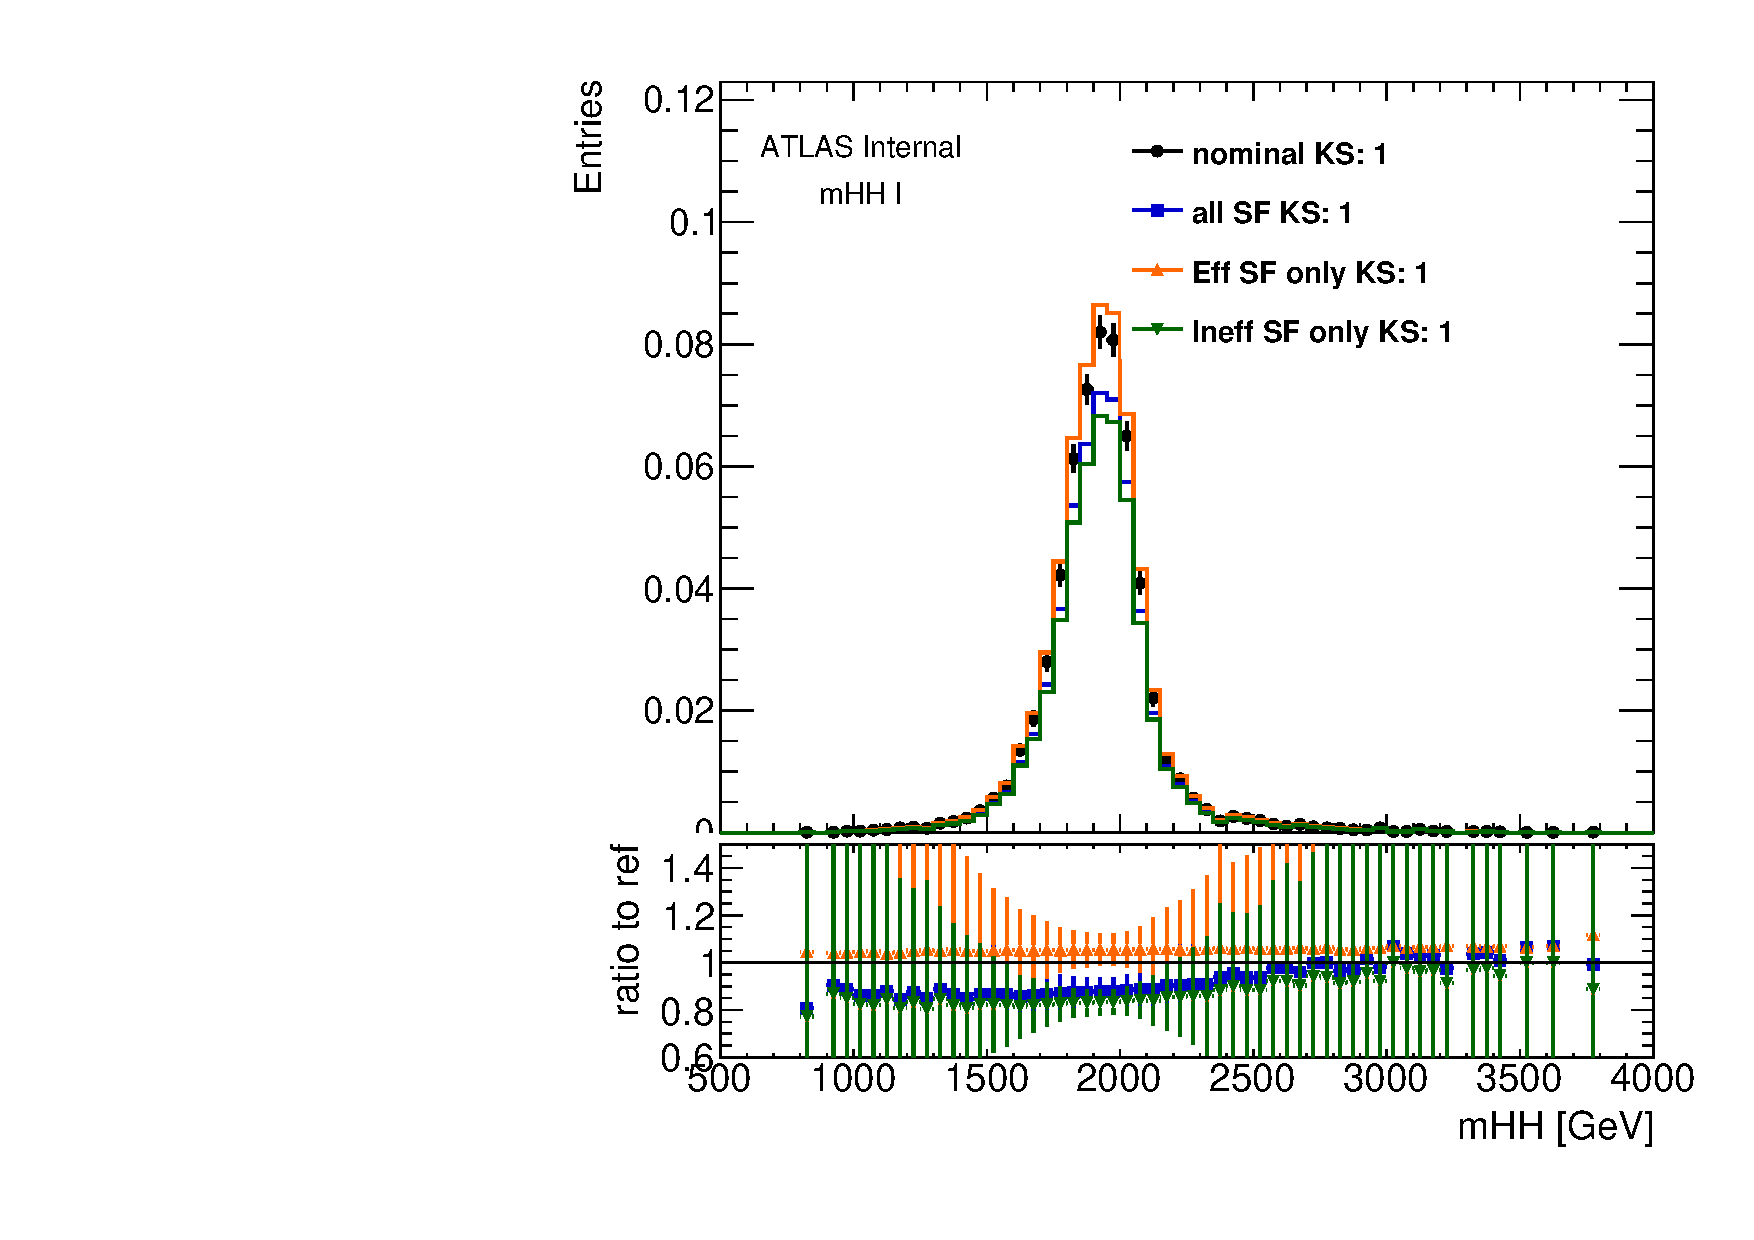
\includegraphics[width=0.31\textwidth,angle=-90]{figures/boosted/AppendixbSF/directcompare_mHH_l_bSF_2000_FT_EFF_Eigen_B_0__1down_TwoTag_split_.pdf}
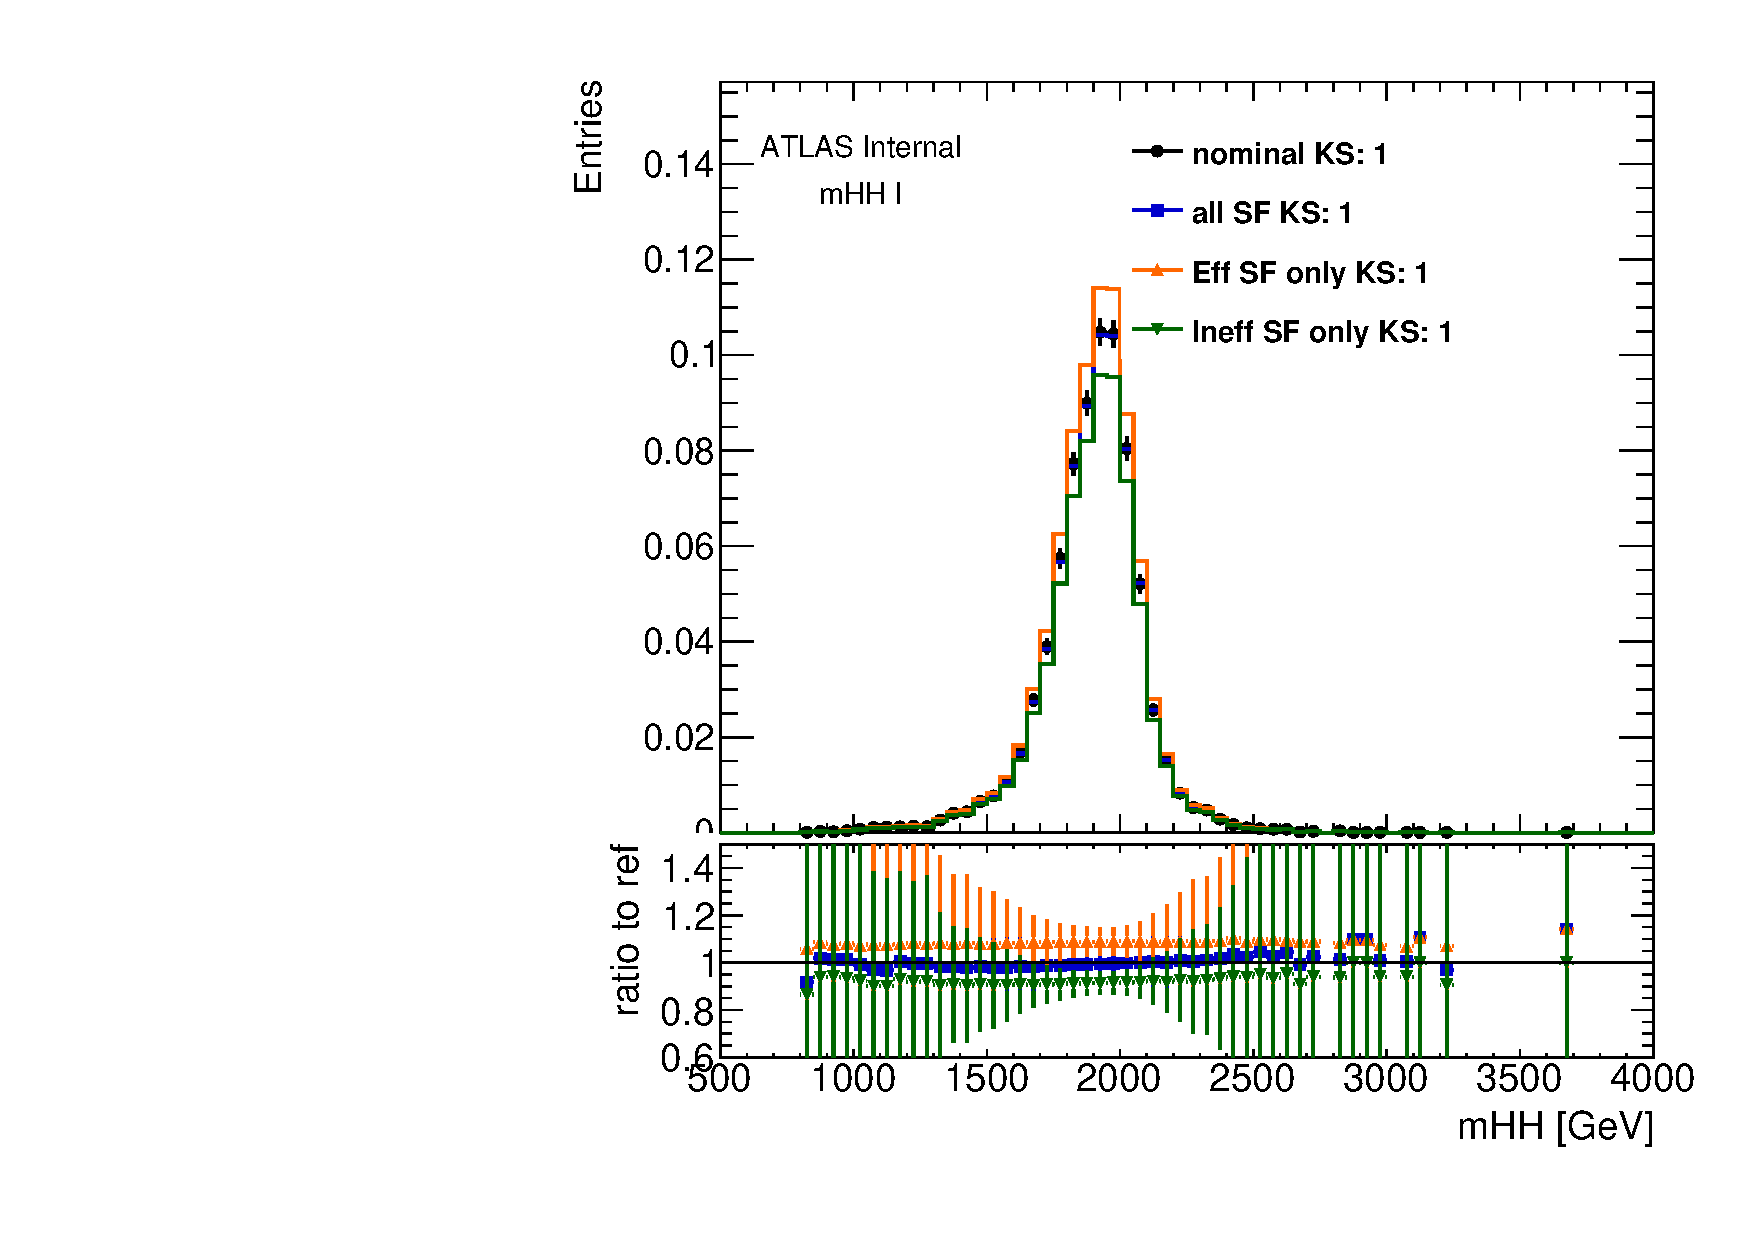
\includegraphics[width=0.31\textwidth,angle=-90]{figures/boosted/AppendixbSF/directcompare_mHH_l_bSF_2000_FT_EFF_Eigen_B_0__1down_ThreeTag_.pdf}
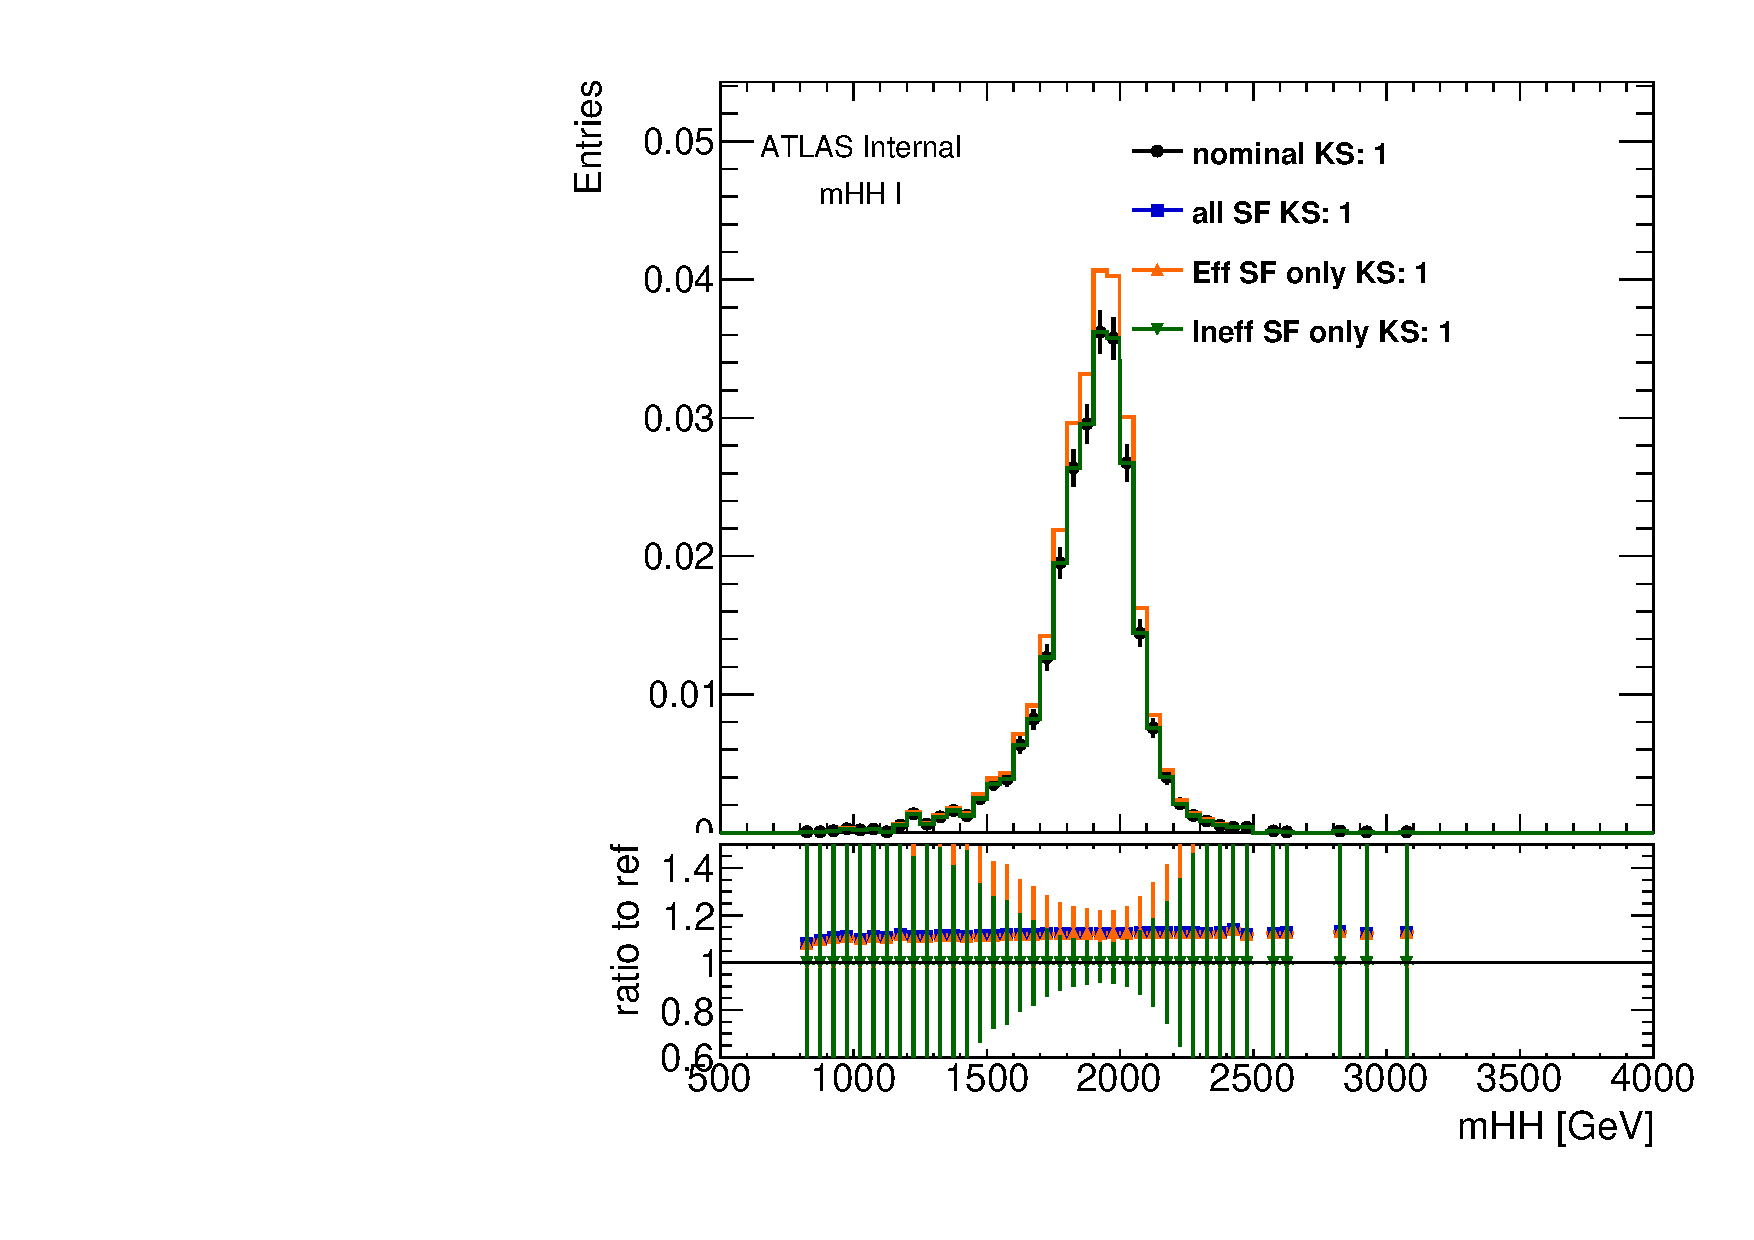
\includegraphics[width=0.31\textwidth,angle=-90]{figures/boosted/AppendixbSF/directcompare_mHH_l_bSF_2000_FT_EFF_Eigen_B_0__1down_FourTag_.pdf}
\caption{Impact of efficiency scale factor $w_{sf}$ and inefficiency scale factor $w_{sf}^{anti}$ on $2$ \TeV~ \Grav~ with $c=1.0$. $4b$ signal region (left), $3b$ signal region (middle), and $2bs$ signal region are shown.}
\label{fig:signal_bsyst_reduction}
\end{center}
\end{figure}
%%%%%%%%%%%%%%%%%%%%%%%%%%%%%%%%%%%%%%%%%%%%%%%%%%%%%%%%%%%%%%%%%%%%%%%
%%%%%%%%%%%%%%%%%%%%%%%%%%%%%%%%%%%%%%%%%%%%%%%%%%%%%%%%%%%%%%%%%%%%%%%
\section{Uncertainty on \ttbar~ generator}
\label{sec:ttbar-mc-unc}

\paragraph{}
In addition to the \ttbar fit uncertainties, following the recommendations, extra \ttbar MC samples are used with different variations: hadronization, fragmentation, matrix element variation and additional radiation.
The top quark mass variations are also considered. 

\paragraph{}
These \ttbar~ samples are used to replace the normal had and non-had MCs, stitched with $m_{t\bar{t}}$ slices samples, and the variation in the \ttbar~ yield and background predictions are considered. 
The variation in total background, with different \ttbar~ MC sample as input is tested. 
This is shown in Figure ~\ref{fig:ttbar-MC}. 
This uncertainty is considered limited by the MC statistics and not included.

\begin{figure}[htbp!]
\begin{center} 
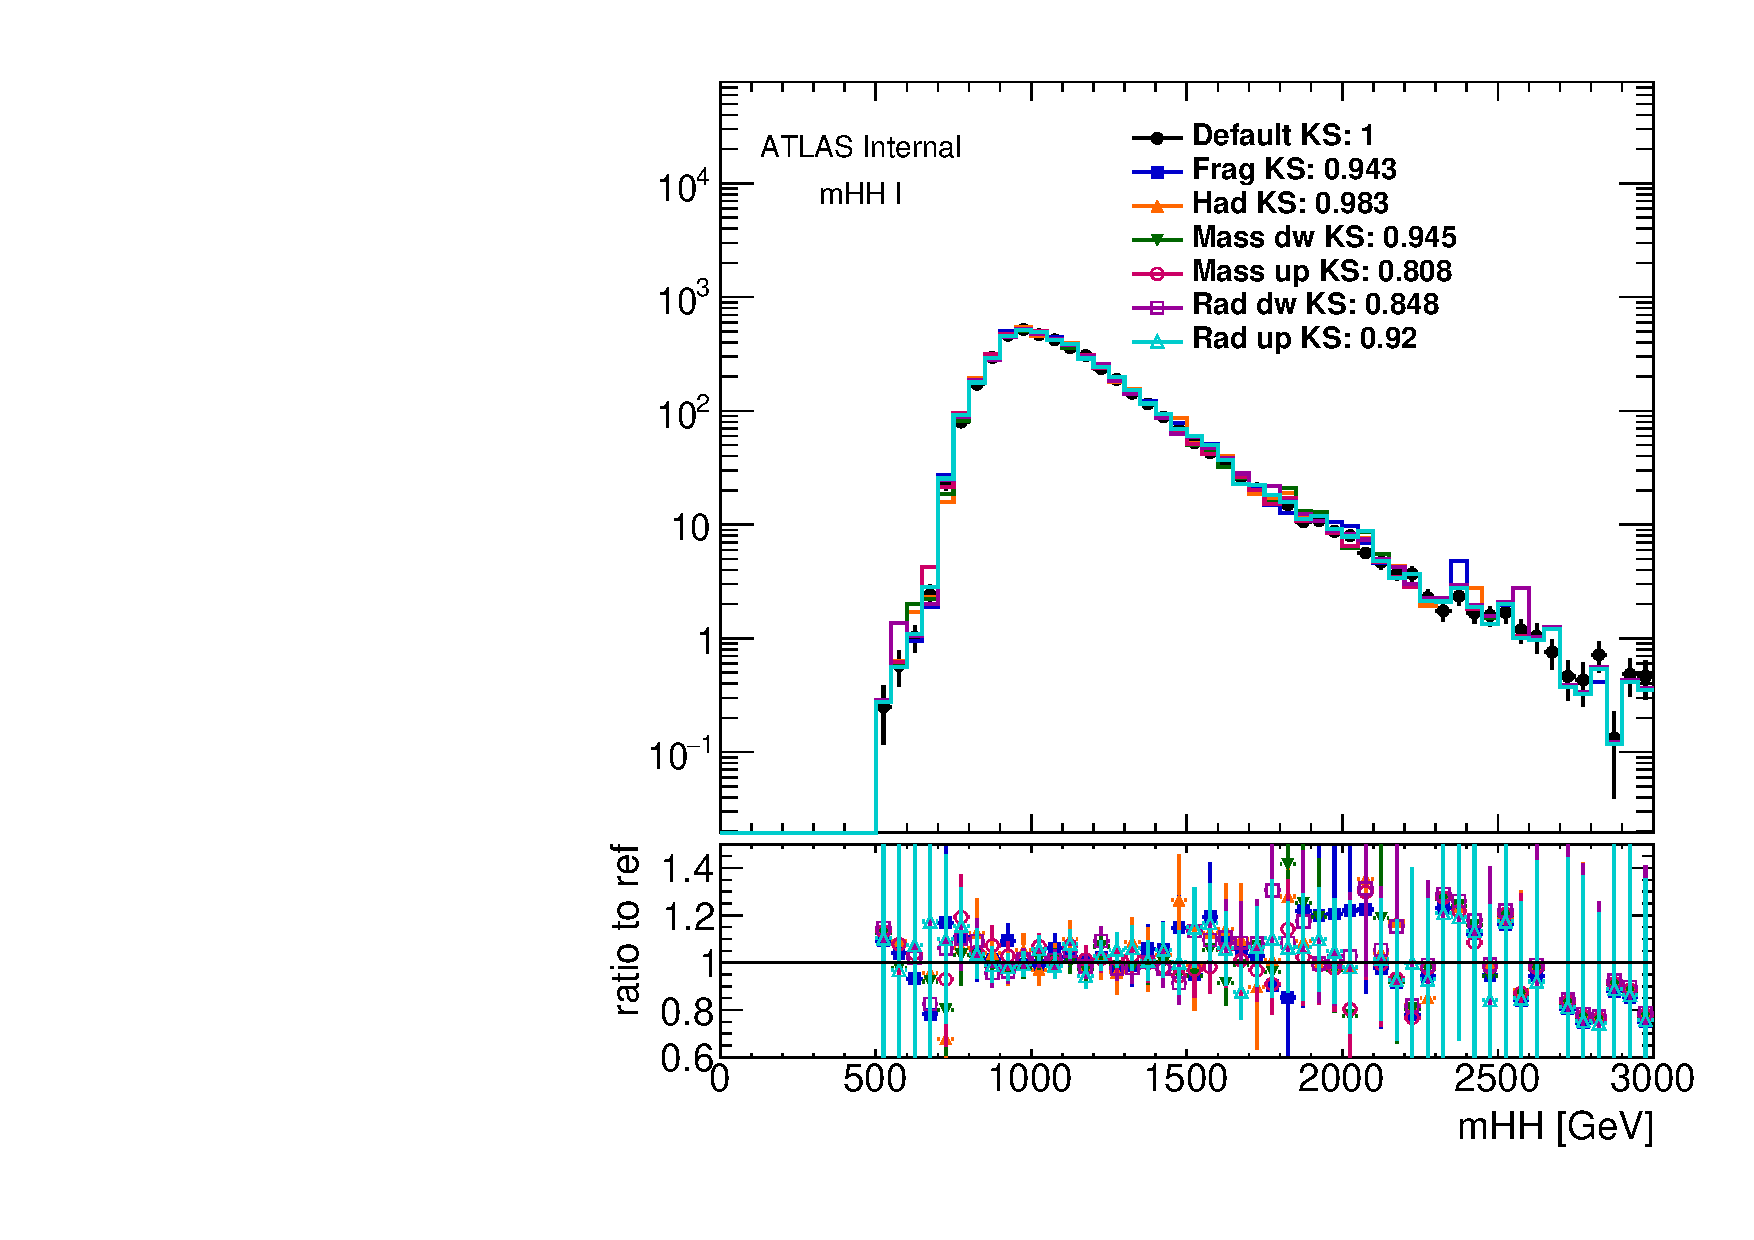
\includegraphics[width=0.48\textwidth,angle=-90]{figures/boosted/Other/directcompare_mHH_l_1_TwoTag_split_Top_syst_stat_postfit_all_.pdf}
\caption{Total background estimation (qcd + \ttbar) with different \ttbar MC variations. The different variations agree with the default within the statistical uncertainties.}
\label{fig:ttbar-MC}
\end{center}
\end{figure}


%%%%%%%%%%%%%%%%%%%%%%%%%%%%%%%%%%%%%%%%%%%%%%%%%%%%%%%%%%%%%%%%%%%%%%%
%%%%%%%%%%%%%%%%%%%%%%%%%%%%%%%%%%%%%%%%%%%%%%%%%%%%%%%%%%%%%%%%%%%%%%%

\section{Uncertainty on \muqcd estimation}
\label{sec:non-closure-mu-qcd}

\paragraph{}
A further uncertainty is derived by comparing the value of \muqcd to the overall difference between predicted to observed events in the control region, shown in section ~\ref{sec:yields}. 
The number events agrees with the total data in the control region within statistical error, but \muqcd~ estimation is dependent on the SB and CR choice,
An additional systematic on the background prediction in the signal region is assigned. 
It is the maximum between either the difference between the central value of the prediction to the observed number of events, or the statistical uncertainty of the observed data in the CR.
For $4b$ it is $11.1\%$, for $3b$ it is $2.5\%$, and for $2bs$ it is $1.1\%$. 

\paragraph{}
Besides the nominal control region, additional sideband and control region are designed and tested. 
They are further illustrated in Appendix~\ref{app:appendixSysVar}, and are listed below:
\begin{itemize}
	\item Low-mass CR: the center position of the circle that defines nominal CR is moved down by 3 GeV, in both leading and sub-leading large-jet mass.
	\item High-mass CR: the center position of the circle that defines nominal CR is moved up by 3 GeV, in both leading and sub-leading large-R jet mass.
	\item Signal-depletion (Small) CR: the $X_{hh}$ cut that defines signal region is increased to $2.0$ from $1.6$. This variation only affect CR, while SR remains unchanged (i.e. signal region is still defined by $X_{hh}<1.6$, while CR is defined as $X_{hh}>2.0$ and $R_{hh}<33$).
	\item High-mass SB: The signal region and control region remain unchanged, the center position of the circle that defines nominal SB is moved up by 3 GeV in both leading and sub-leading large-R jet mass.
	\item Low-mass SB: The signal region and control region remain unchanged, the center position of the circle that defines nominal SB is moved up by 3 GeV in both leading and sub-leading large-R jet mass.
	\item Large SB: The signal region and control region remain unchanged, while the SB is $33 < R_{hh}$ and $ R_{hh}^{\text{high}} < 61$. $\mu_{QCD}$ will change.
	\item Small SB: The signal region and control region remain unchanged, while the SB is $33 < R_{hh}$ and $ R_{hh}^{\text{high}} < 55$. $\mu_{QCD}$ will change.
\end{itemize}

\paragraph{}
To ensure that these value cover the QCD normalization uncertainty, further checks on the effect of adjusting the control and sideband definitions were done. 
All these tests are done on the control/sideband regions after the full reweighting procedure as described in \ref{sec:boosted-reweight}, while applying the nominal reweighting values.
The results are summarized in Table \ref{CRSB:Tab_4b_CR_Variations}, \ref{CRSB:Tab_3b_CR_Variations} and \ref{CRSB:Tab_2bs_CR_Variations}. 
Based on all the variations, a final $2.8\%$ normalization uncertainty is assigned to $2bs$ signal region, $4.2\%$ to $3b$ signal region, and a $12.2\%$ normalization uncertainty is assigned to $4b$ signal region.

\begin{table}[htbp!]
\begin{center}
\begin{footnotesize} 
\begin{tabular}{c|c|c|c} 
CR Varations FourTag & Data & Prediction & (Predict - Data)/Data \\ 
\hline\hline 
& & & \\ 
Nominal & 81.0 $\pm$ 9.0 & 76.77 $\pm$ 5.43 & -5.22 $\%$  $\pm$ 17.23 $\%$ \\ 
\hline 
CR High & 76.0 $\pm$ 8.72 & 71.12 $\pm$ 5.41 & -6.43 $\%$  $\pm$ 17.85 $\%$ \\ 
\hline 
CR Low & 91.0 $\pm$ 9.54 & 79.87 $\pm$ 5.45 & -12.2 $\%$  $\pm$ 15.19 $\%$ \\ 
\hline 
CR Small & 58.0 $\pm$ 7.62 & 55.96 $\pm$ 5.35 & -3.52 $\%$  $\pm$ 21.89 $\%$ \\ 
\hline 
SB Large & 81.0 $\pm$ 9.0 & 74.71 $\pm$ 5.4 & -7.76 $\%$  $\pm$ 16.91 $\%$ \\ 
\hline 
SB Small & 81.0 $\pm$ 9.0 & 74.15 $\pm$ 5.38 & -8.45 $\%$  $\pm$ 16.81 $\%$ \\ 
\hline 
SB High & 81.0 $\pm$ 9.0 & 78.72 $\pm$ 5.46 & -2.82 $\%$  $\pm$ 17.54 $\%$ \\ 
\hline 
SB Low & 81.0 $\pm$ 9.0 & 76.51 $\pm$ 5.38 & -5.54 $\%$  $\pm$ 17.14 $\%$ \\ 
& & & \\ 
\hline\hline 
\end{tabular} 
\end{footnotesize} 
\newline 

\end{center}
\caption{Agreement between data and prediction in $4b$ tag CR. Showing stat uncertainty only.}
\label{CRSB:Tab_4b_CR_Variations}
\end{table}

\begin{table}[htbp!]
\begin{center}
\begin{footnotesize} 
\begin{tabular}{c|c|c|c} 
CR Varations ThreeTag & Data & Prediction & (Predict - Data)/Data \\ 
\hline\hline 
Nominal & 1553.0 $\pm$ 39.41 & 1587.04 $\pm$ 21.4 & 2.19 $\%$  $\pm$ 3.97 $\%$ \\ 
\hline 
CR High & 1461.0 $\pm$ 38.22 & 1473.89 $\pm$ 20.77 & 0.88 $\%$  $\pm$ 4.06 $\%$ \\ 
\hline 
CR Low & 1628.0 $\pm$ 40.35 & 1697.38 $\pm$ 21.75 & 4.26 $\%$  $\pm$ 3.92 $\%$ \\ 
\hline 
CR Small & 1134.0 $\pm$ 33.67 & 1127.34 $\pm$ 17.66 & -0.59 $\%$  $\pm$ 4.51 $\%$ \\ 
\hline 
SB Large & 1553.0 $\pm$ 39.41 & 1574.23 $\pm$ 21.47 & 1.37 $\%$  $\pm$ 3.95 $\%$ \\ 
\hline 
SB Small & 1553.0 $\pm$ 39.41 & 1601.44 $\pm$ 21.64 & 3.12 $\%$  $\pm$ 4.01 $\%$ \\ 
\hline 
SB High & 1553.0 $\pm$ 39.41 & 1602.74 $\pm$ 21.48 & 3.2 $\%$  $\pm$ 4.0 $\%$ \\ 
\hline 
SB Low & 1553.0 $\pm$ 39.41 & 1576.56 $\pm$ 21.5 & 1.52 $\%$  $\pm$ 3.96 $\%$ \\ 
\hline\hline 
\end{tabular} 
\end{footnotesize} 
\newline 

\end{center}
\caption{Agreement between data and prediction in $3b$ tag CR. Showing stat uncertainty only.}
\label{CRSB:Tab_3b_CR_Variations}
\end{table}
\begin{table}[htbp!]
\begin{center}
\begin{footnotesize} 
\begin{tabular}{c|c|c|c} 
CR Varations TwoTag split & Data & Prediction & (Predict - Data)/Data \\ 
\hline\hline 
& & & \\ 
Nominal & 8486.0 $\pm$ 92.12 & 8332.97 $\pm$ 38.84 & -1.8 $\%$  $\pm$ 1.52 $\%$ \\ 
\hline 
CR High & 8174.0 $\pm$ 90.41 & 7937.59 $\pm$ 39.61 & -2.89 $\%$  $\pm$ 1.56 $\%$ \\ 
\hline 
CR Low & 8907.0 $\pm$ 94.38 & 8800.86 $\pm$ 39.51 & -1.19 $\%$  $\pm$ 1.49 $\%$ \\ 
\hline 
CR Small & 5999.0 $\pm$ 77.45 & 5873.52 $\pm$ 32.31 & -2.09 $\%$  $\pm$ 1.8 $\%$ \\ 
\hline 
SB Large & 8486.0 $\pm$ 92.12 & 8341.7 $\pm$ 38.44 & -1.7 $\%$  $\pm$ 1.52 $\%$ \\ 
\hline 
SB Small & 8486.0 $\pm$ 92.12 & 8333.25 $\pm$ 39.12 & -1.8 $\%$  $\pm$ 1.53 $\%$ \\ 
\hline 
SB High & 8486.0 $\pm$ 92.12 & 8378.14 $\pm$ 38.45 & -1.27 $\%$  $\pm$ 1.52 $\%$ \\ 
\hline 
SB Low & 8486.0 $\pm$ 92.12 & 8356.86 $\pm$ 39.06 & -1.52 $\%$  $\pm$ 1.53 $\%$ \\ 
& & & \\ 
\hline\hline 
\end{tabular} 
\end{footnotesize} 
\newline 

\end{center}
\caption{Agreement between data and prediction in $2bs$ tag CR. Showing stat uncertainty only.}
\label{CRSB:Tab_2bs_CR_Variations}
\end{table}


%%%%%%%%%%%%%%%%%%%%%%%%%%
\section{Validation in low mass and high mass signal region}
\label{sec:boosted-ZZ-Rehearsal}
\paragraph{}
Another check is the the so-called ``low mass signal region'' (or ZZ region) and ``high mass signal region'' (or TT region). 
Instead of the signal region around di-Higgs mass region on \mleadJ-\msublJ large-\R jet mass 2D plane, a separate lower mass (ZZ) and higher mass (TT) signal region are defined: 
\begin{equation}
X_{ZZ} = \sqrt{\left(\frac{m^{\rm lead}_{\rm J} - \text{103 GeV}}{0.1 \left(m^{\rm lead}_{\rm J}\right)}\right)^2 + \left(\frac{m^{\rm subl}_{\rm J}- \text{96 GeV}}{0.1 \left(m^{\rm subl}_{\rm J}\right)}\right)^2}
\label{eq:boosted_Xzz}
\end{equation}
\begin{equation}
X_{TT} = \sqrt{\left(\frac{m^{\rm lead}_{\rm J} - \text{164 GeV}}{0.1 \left(m^{\rm lead}_{\rm J}\right)}\right)^2 + \left(\frac{m^{\rm subl}_{\rm J}- \text{155 GeV}}{0.1 \left(m^{\rm subl}_{\rm J}\right)}\right)^2}
\label{eq:boosted_Xtt}
\end{equation}
which is also illustrated in Figure \ref{CRSB:ZZIllustration}. 
The analysis is repeated, using the same definition of sideband and control region as the nominal (but with events contained in ZZ signal region excluded) for normalization fit. 
Then the low mass signal region is unblinded. 
This helps to validate the background estimation strategy, and the stability for other similar analysis.

\begin{figure}[htbp!]
\begin{center}
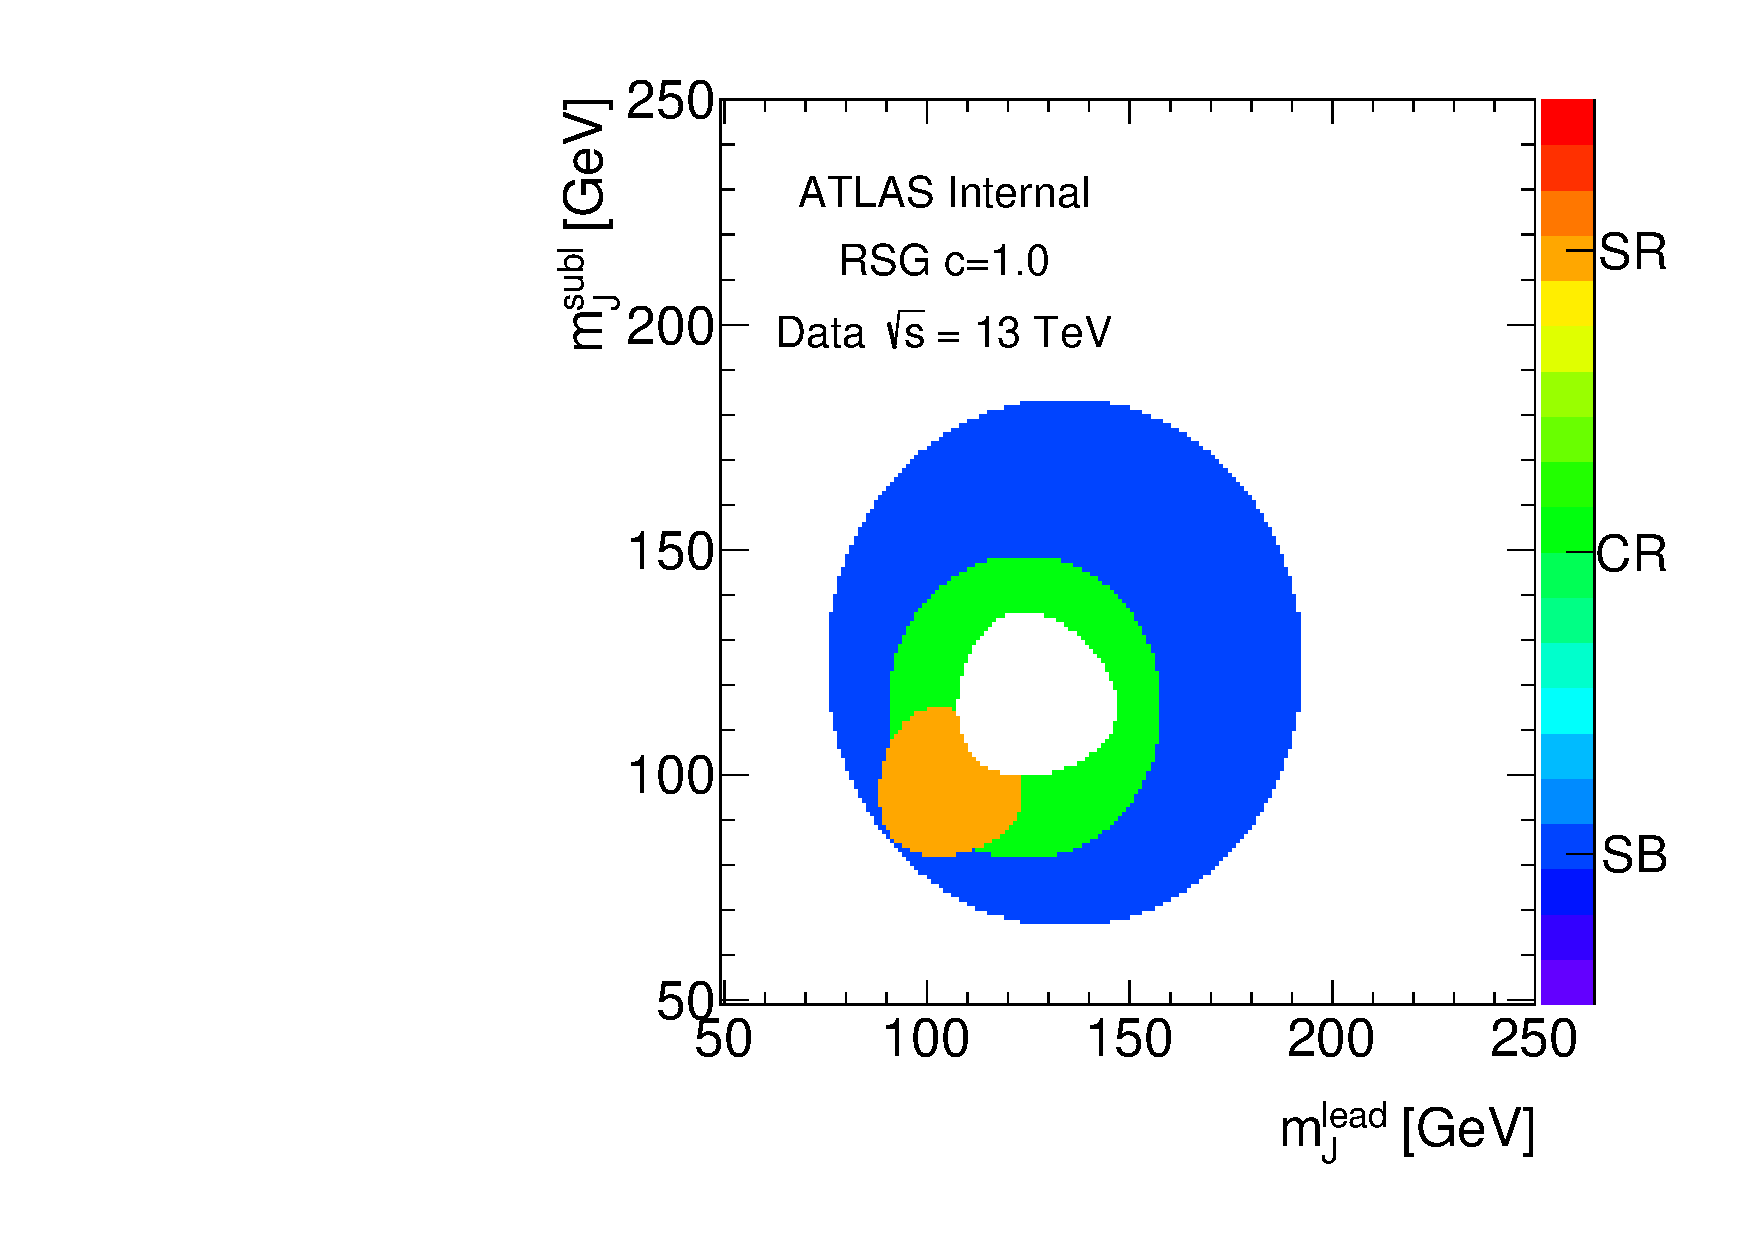
\includegraphics[width=0.4\textwidth,angle=-90]{figures/boosted/ZZ/Compare_NoTag_mH0H1.pdf}
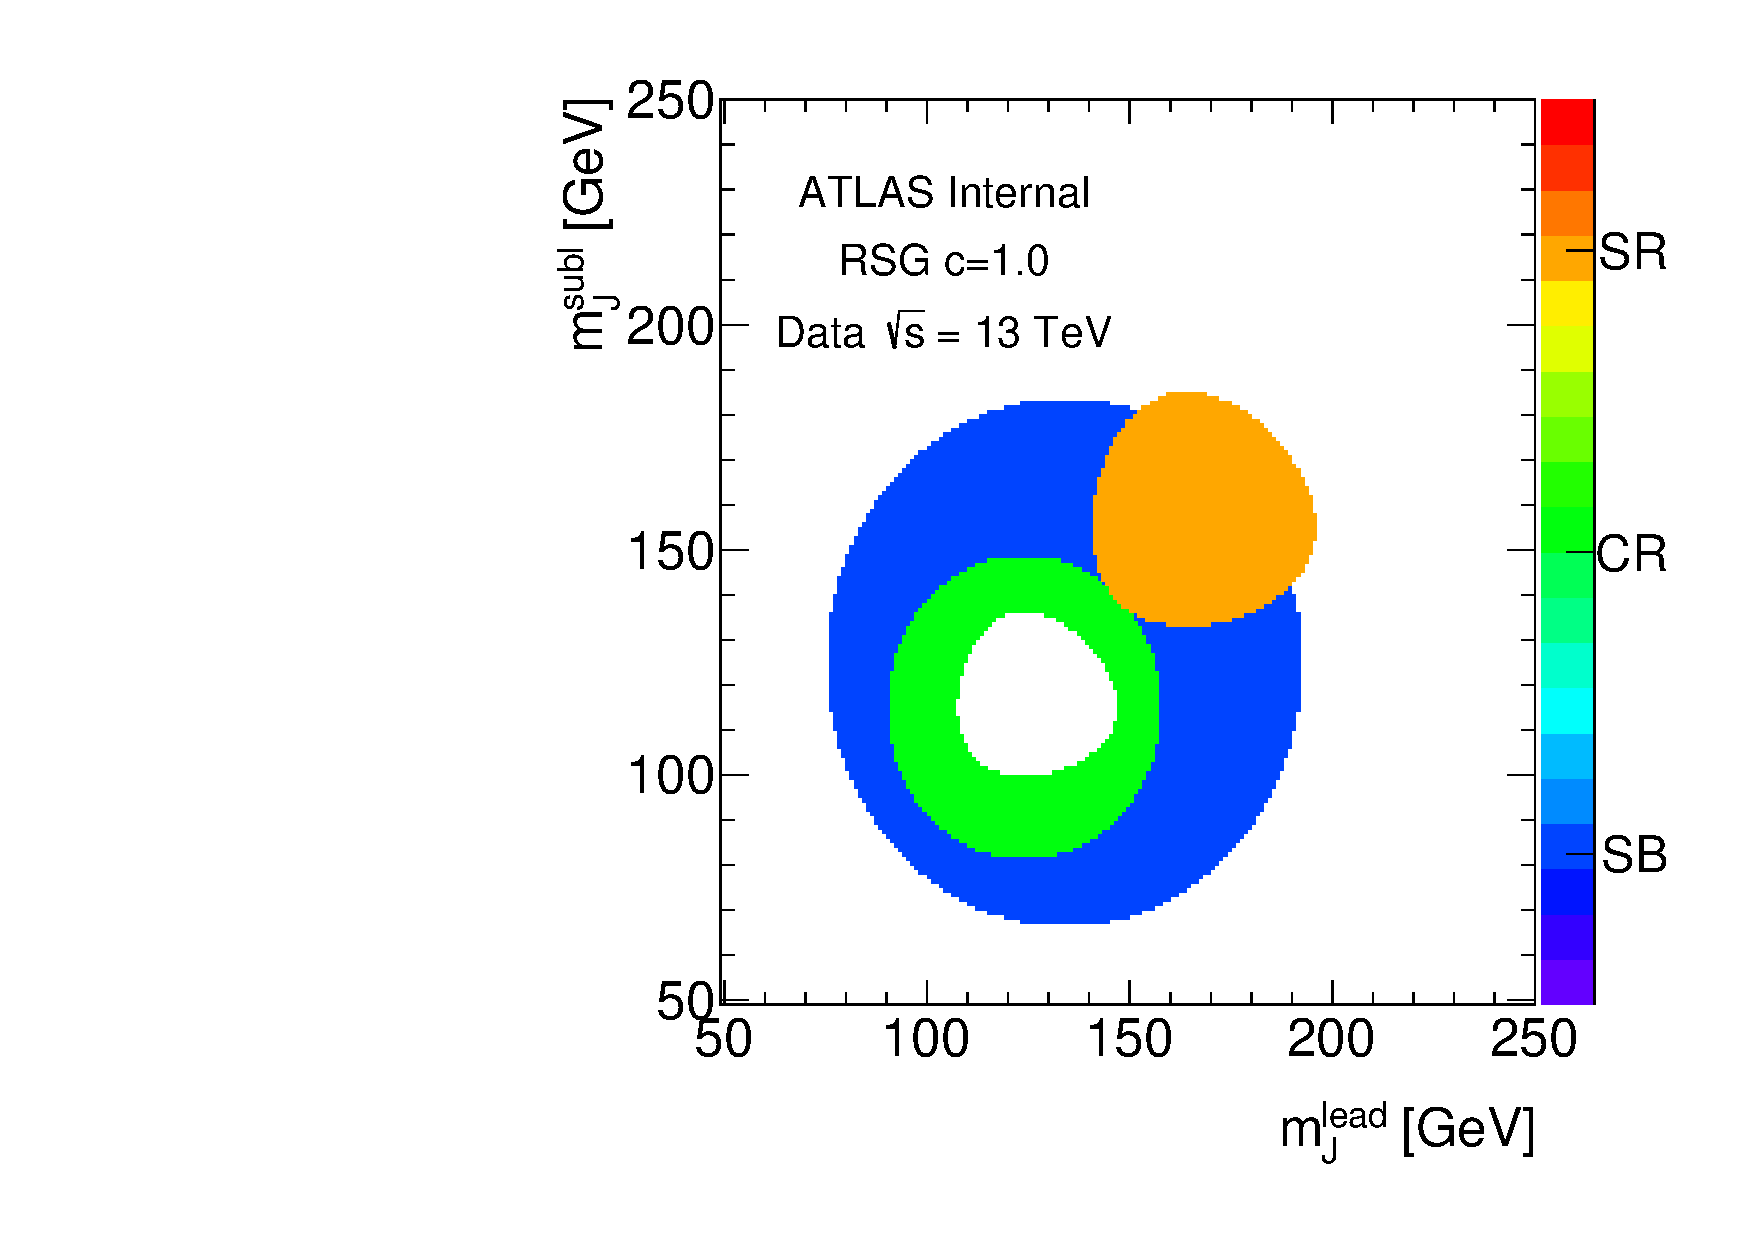
\includegraphics[width=0.4\textwidth,angle=-90]{figures/boosted/TT/Compare_NoTag_mH0H1.pdf}
\end{center}
\caption{Illustration of ZZ (left) and TT (right) signal region as shown in the orange shaded region. Control region shown in green, and sideband region in blue. The white circle in the middle is the real signal region, and it is blinded.}
\label{CRSB:ZZIllustration}
\end{figure}

\paragraph{}
%The summary of background estimation for ZZ signal region can be found in Table \ref{CRSB:SummaryTable_ZZ_4b}, ~\ref{CRSB:SummaryTable_ZZ_3b} and ~\ref{CRSB:SummaryTable_ZZ_2b}. 
The difference between data and prediction in ZZ signal region is summarized in Table \ref{CRSB:DataPred_ZZSR} for all the regions. T
he discrepancy between data and prediction is either covered by statistical uncertainty of data or comparable with data statistical uncertainty in $4b$, $3b$ and $2bs$ ZZ SR respectively. 
The kinematic distribution between data and prediction in ZZ SR are shown in Figure \ref{CRSB:ZZSR_Distribution}. 
The data agrees with prediction well in general, though a few bins might not agree perfectly. 
The difference from $4b$ CR region test is 17$\%$, which is smaller than the $4b$ ZZ region difference. 
But the statistical uncertainty in ZZ region (with yield 37) is much higher compared with the CR regions (with minimum yield 76), hence the CR region with more statistical power is still used for the non-closure uncertainty.

\paragraph{}
%The summary of background estimation for TT signal region can be found in Table \ref{CRSB:SummaryTable_TT_4b}, ~\ref{CRSB:SummaryTable_TT_3b} and ~\ref{CRSB:SummaryTable_TT_2b}.
The difference between data and prediction in TT signal region is summarized in Table \ref{CRSB:DataPred_TTSR} for all the regions. 
The discrepancy between data and prediction is either covered by statistical uncertainty of data or comparable with data statistical uncertainty in $4b$, $3b$ and $2bs$ TT SR respectively. 
The kinematic distribution between data and prediction in TT SR are shown in Figure \ref{CRSB:TTSR_Distribution}. 
The data agrees with prediction well in general, though a few bins might not agree perfectly. 

\paragraph{}
Based on all the variation tests, there is no need to introduce extra uncertainty on non-closure systematics. 
Most of the data/prediction disagreements are well covered by the data statistical uncertainty.

% \begin{table}[htbp!]
% \begin{center}
% \begin{footnotesize} 
\begin{tabular}{c|c|c|c} 
FourTag & Sideband & Control & Signal \\ 
\hline\hline 
QCD Est & 166.65 $\pm$ 2.88 & 45.83 $\pm$ 1.51 & 27.37 $\pm$ 1.16\\ 
$t\bar{t}$ Est.  & 27.52 $\pm$ 0.25 & 6.31 $\pm$ 0.14 & 0 $\pm$ 0\\ 
$Z+jets$ & 0 $\pm$ 0 & 6.18 $\pm$ 5.12 & 0 $\pm$ 0\\ 
Total Bkg Est & 194.17 $\pm$ 2.89 & 58.32 $\pm$ 5.34 & 27.37 $\pm$ 1.16\\ 
Data & 194.0 $\pm$ 13.93 & 54.0 $\pm$ 7.35 & 37.0 $\pm$ 6.08\\ 
$c=1.0$,$m=1.0TeV$ & 2.45 $\pm$ 0.098 & 4.47 $\pm$ 0.13 & 0.99 $\pm$ 0.063\\ 
$c=1.0$,$m=2.0TeV$ & 0.032 $\pm$ 0.0015 & 0.075 $\pm$ 0.0022 & 0.028 $\pm$ 0.0014\\ 
$c=1.0$,$m=3.0TeV$ & 0.00029 $\pm$ 3.5e-05 & 0.00064 $\pm$ 5e-05 & 0.0002 $\pm$ 2.7e-05\\ 
\hline\hline 
\end{tabular} 
\end{footnotesize} 
\newline 

% \end{center}
% \caption{Background prediction in SR/CR/SB for ZZ SR in $4b$-tag region. Uncertainties are stat only.}
% \label{CRSB:SummaryTable_ZZ_4b}
% \end{table}

% \begin{table}[htbp!]
% \begin{center}
% \begin{footnotesize} 
\begin{tabular}{c|c|c|c} 
ThreeTag & Sideband & Control & Signal \\ 
\hline\hline 
& & & \\ 
QCD Est & 3344.46 $\pm$ 26.85 & 998.41 $\pm$ 14.63 & 637.78 $\pm$ 11.87\\ 
$t\bar{t}$ Est.  & 826.66 $\pm$ 25.11 & 136.58 $\pm$ 10.23 & 30.07 $\pm$ 1.24\\ 
$Z+jets$ & 32.49 $\pm$ 11.34 & 8.22 $\pm$ 5.29 & 3.3 $\pm$ 2.0\\ 
Total Bkg Est & 4203.61 $\pm$ 38.47 & 1143.2 $\pm$ 18.62 & 671.15 $\pm$ 12.11\\ 
Data & 4203.0 $\pm$ 64.83 & 1108.0 $\pm$ 33.29 & 645.0 $\pm$ 25.4\\ 
$c=1.0$,$m=1.0TeV$ & 7.56 $\pm$ 0.18 & 9.84 $\pm$ 0.2 & 3.05 $\pm$ 0.11\\ 
$c=1.0$,$m=2.0TeV$ & 0.15 $\pm$ 0.0033 & 0.27 $\pm$ 0.0046 & 0.12 $\pm$ 0.003\\ 
$c=1.0$,$m=3.0TeV$ & 0.0034 $\pm$ 0.00012 & 0.0056 $\pm$ 0.00016 & 0.0021 $\pm$ 9.5e-05\\ 
& & & \\ 
\hline\hline 
\end{tabular} 
\end{footnotesize} 
\newline 

% \end{center}
% \caption{Background prediction in SR/CR/SB for ZZ SR in $3b$-tag region. Uncertainties are stat only.}
% \label{CRSB:SummaryTable_ZZ_3b}
% \end{table}

% \begin{table}[htbp!]
% \begin{center}
% \begin{footnotesize} 
\begin{tabular}{c|c|c|c} 
TwoTag split & Sideband & Control & Signal \\ 
\hline\hline 
QCD Est & 16387.44 $\pm$ 37.6 & 4827.76 $\pm$ 19.86 & 3026.83 $\pm$ 15.61\\ 
$t\bar{t}$ Est.  & 7671.95 $\pm$ 69.14 & 1229.96 $\pm$ 26.54 & 332.29 $\pm$ 13.66\\ 
$Z+jets$ & 44.37 $\pm$ 13.23 & 13.34 $\pm$ 6.6 & 36.47 $\pm$ 12.88\\ 
Total Bkg Est & 24103.77 $\pm$ 79.8 & 6071.07 $\pm$ 33.8 & 3395.59 $\pm$ 24.42\\ 
Data & 24104.0 $\pm$ 155.25 & 6261.0 $\pm$ 79.13 & 3258.0 $\pm$ 57.08\\ 
$c=1.0$,$m=1.0TeV$ & 4.57 $\pm$ 0.14 & 4.65 $\pm$ 0.14 & 1.91 $\pm$ 0.089\\ 
$c=1.0$,$m=2.0TeV$ & 0.16 $\pm$ 0.0038 & 0.26 $\pm$ 0.0047 & 0.12 $\pm$ 0.0032\\ 
$c=1.0$,$m=3.0TeV$ & 0.012 $\pm$ 0.00024 & 0.019 $\pm$ 0.00029 & 0.0085 $\pm$ 0.00019\\ 
\hline\hline 
\end{tabular} 
\end{footnotesize} 
\newline 

% \end{center}
% \caption{Background prediction in SR/CR/SB for ZZ SR in $2bs$-tag region. Uncertainties are stat only.}
% \label{CRSB:SummaryTable_ZZ_2b}
% \end{table}

\begin{table}[htbp!]
\caption{Data and prediction in ZZ SR in $4b$, $3b$ and $2bs$ regions.}
\begin{center}
\begin{footnotesize} 
\begin{tabular}{c|c|c|c} 
ZZ Signal Region & Data & Prediction & (Predict - Data)/Data \\ 
\hline\hline 
FourTag & 37.0 $\pm$ 6.08 & 27.37 $\pm$ 1.16 & -26.0 $\%$  $\pm$ 15.3 $\%$ \\ 
\hline 
ThreeTag & 645.0 $\pm$ 25.4 & 671.15 $\pm$ 12.11 & 4.05 $\%$  $\pm$ 5.97 $\%$ \\ 
\hline 
TwoTag split & 3258.0 $\pm$ 57.08 & 3395.59 $\pm$ 24.42 & 4.22 $\%$  $\pm$ 2.58 $\%$ \\ 
\hline\hline 
\end{tabular} 
\end{footnotesize} 
\newline 

\end{center}
\label{CRSB:DataPred_ZZSR}
\end{table}

\begin{table}[htbp!]
\begin{center}
\caption{Data and prediction in TT SR in $4b$, $3b$ and $2bs$ regions.}
\begin{footnotesize} 
\begin{tabular}{c|c|c|c} 
TT Signal Region & Data & Prediction & (Predict - Data)/Data \\ 
\hline\hline 
FourTag & 46.0 $\pm$ 6.78 & 43.62 $\pm$ 1.23 & -5.18 $\%$  $\pm$ 16.66 $\%$ \\ 
\hline 
ThreeTag & 1017.0 $\pm$ 31.89 & 976.88 $\pm$ 12.81 & -3.95 $\%$  $\pm$ 4.27 $\%$ \\ 
\hline 
TwoTag split & 6446.0 $\pm$ 80.29 & 6453.23 $\pm$ 51.41 & 0.11 $\%$  $\pm$ 2.04 $\%$ \\ 
\hline\hline 
\end{tabular} 
\end{footnotesize} 
\newline 

\end{center}
\label{CRSB:DataPred_TTSR}
\end{table}

\begin{figure}[htbp!]
\begin{center}
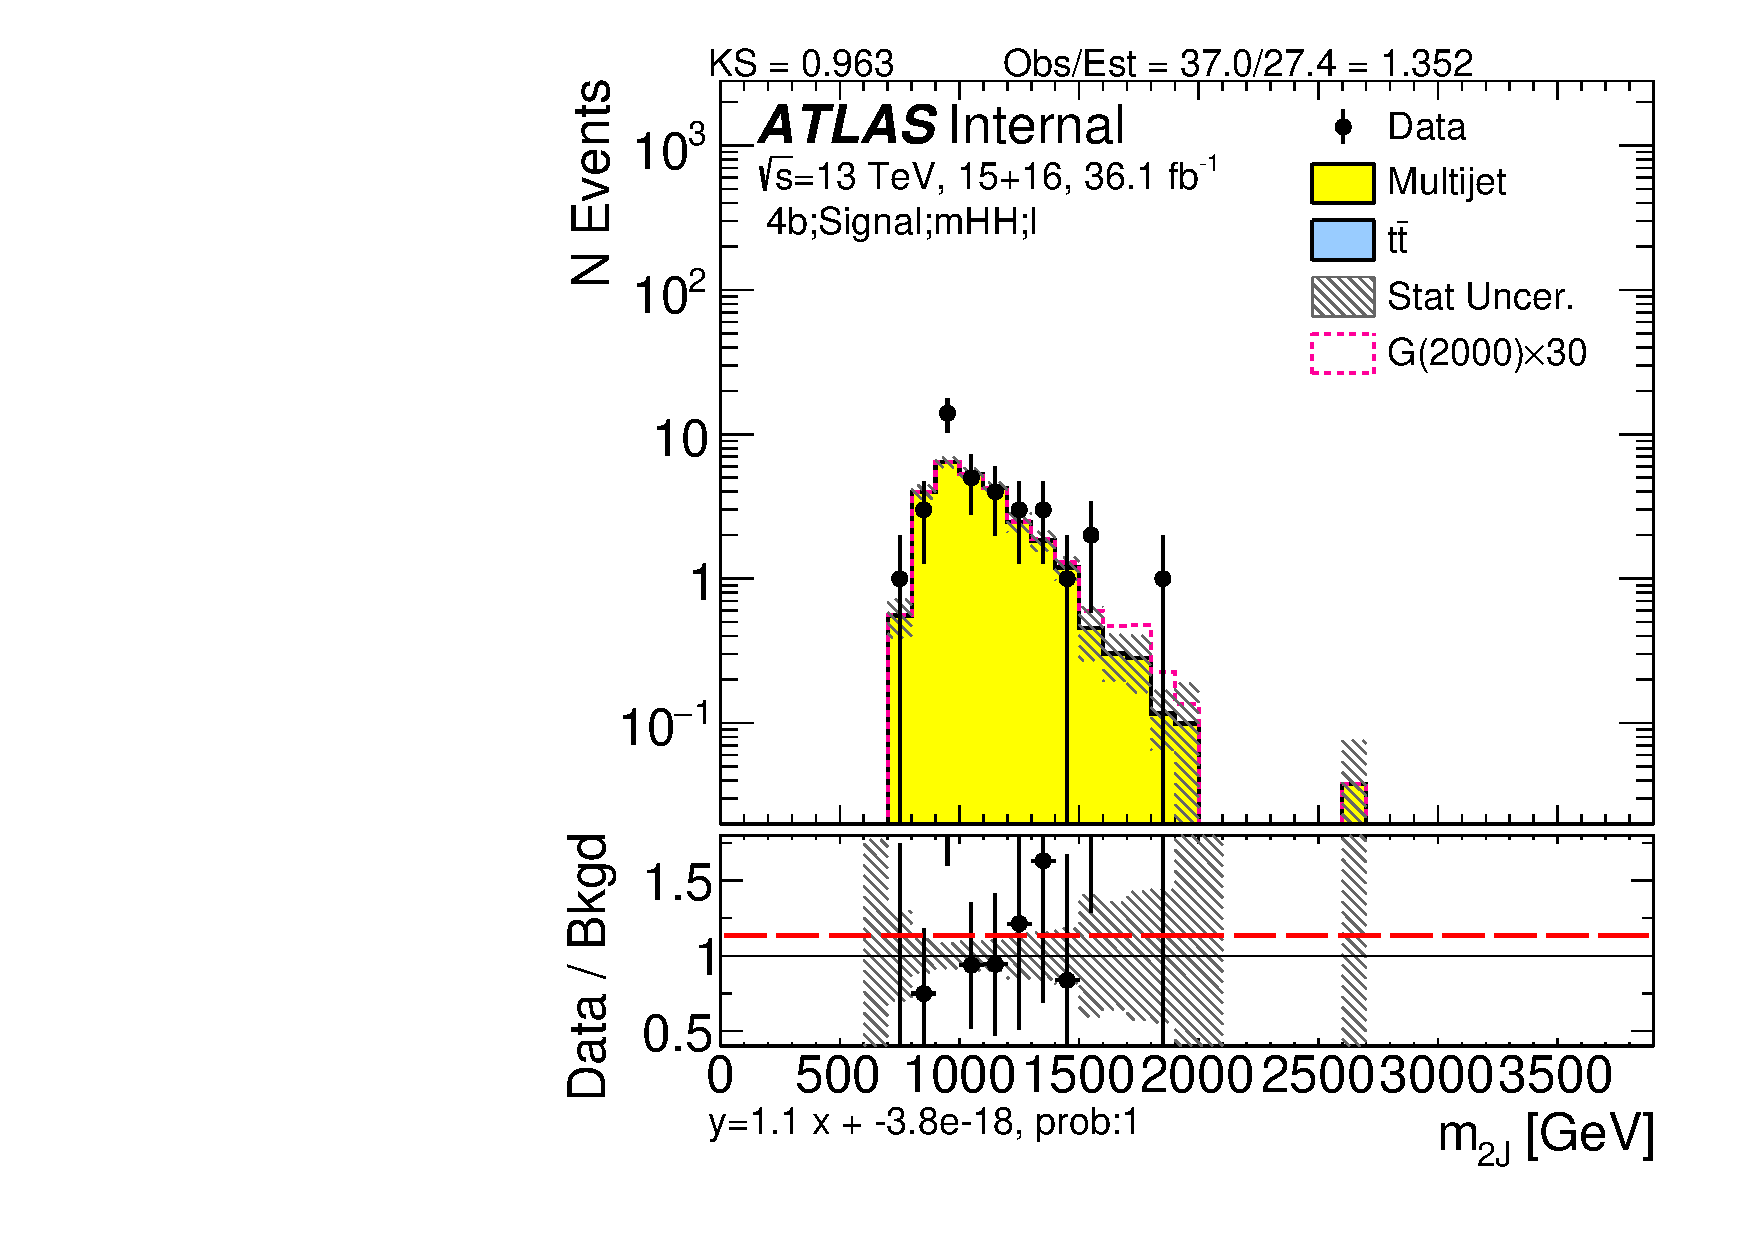
\includegraphics[width=0.45\textwidth,angle=-90]{figures/boosted/ZZ/Moriond_ZZ_FourTag_Signal_mHH_l_1.pdf}
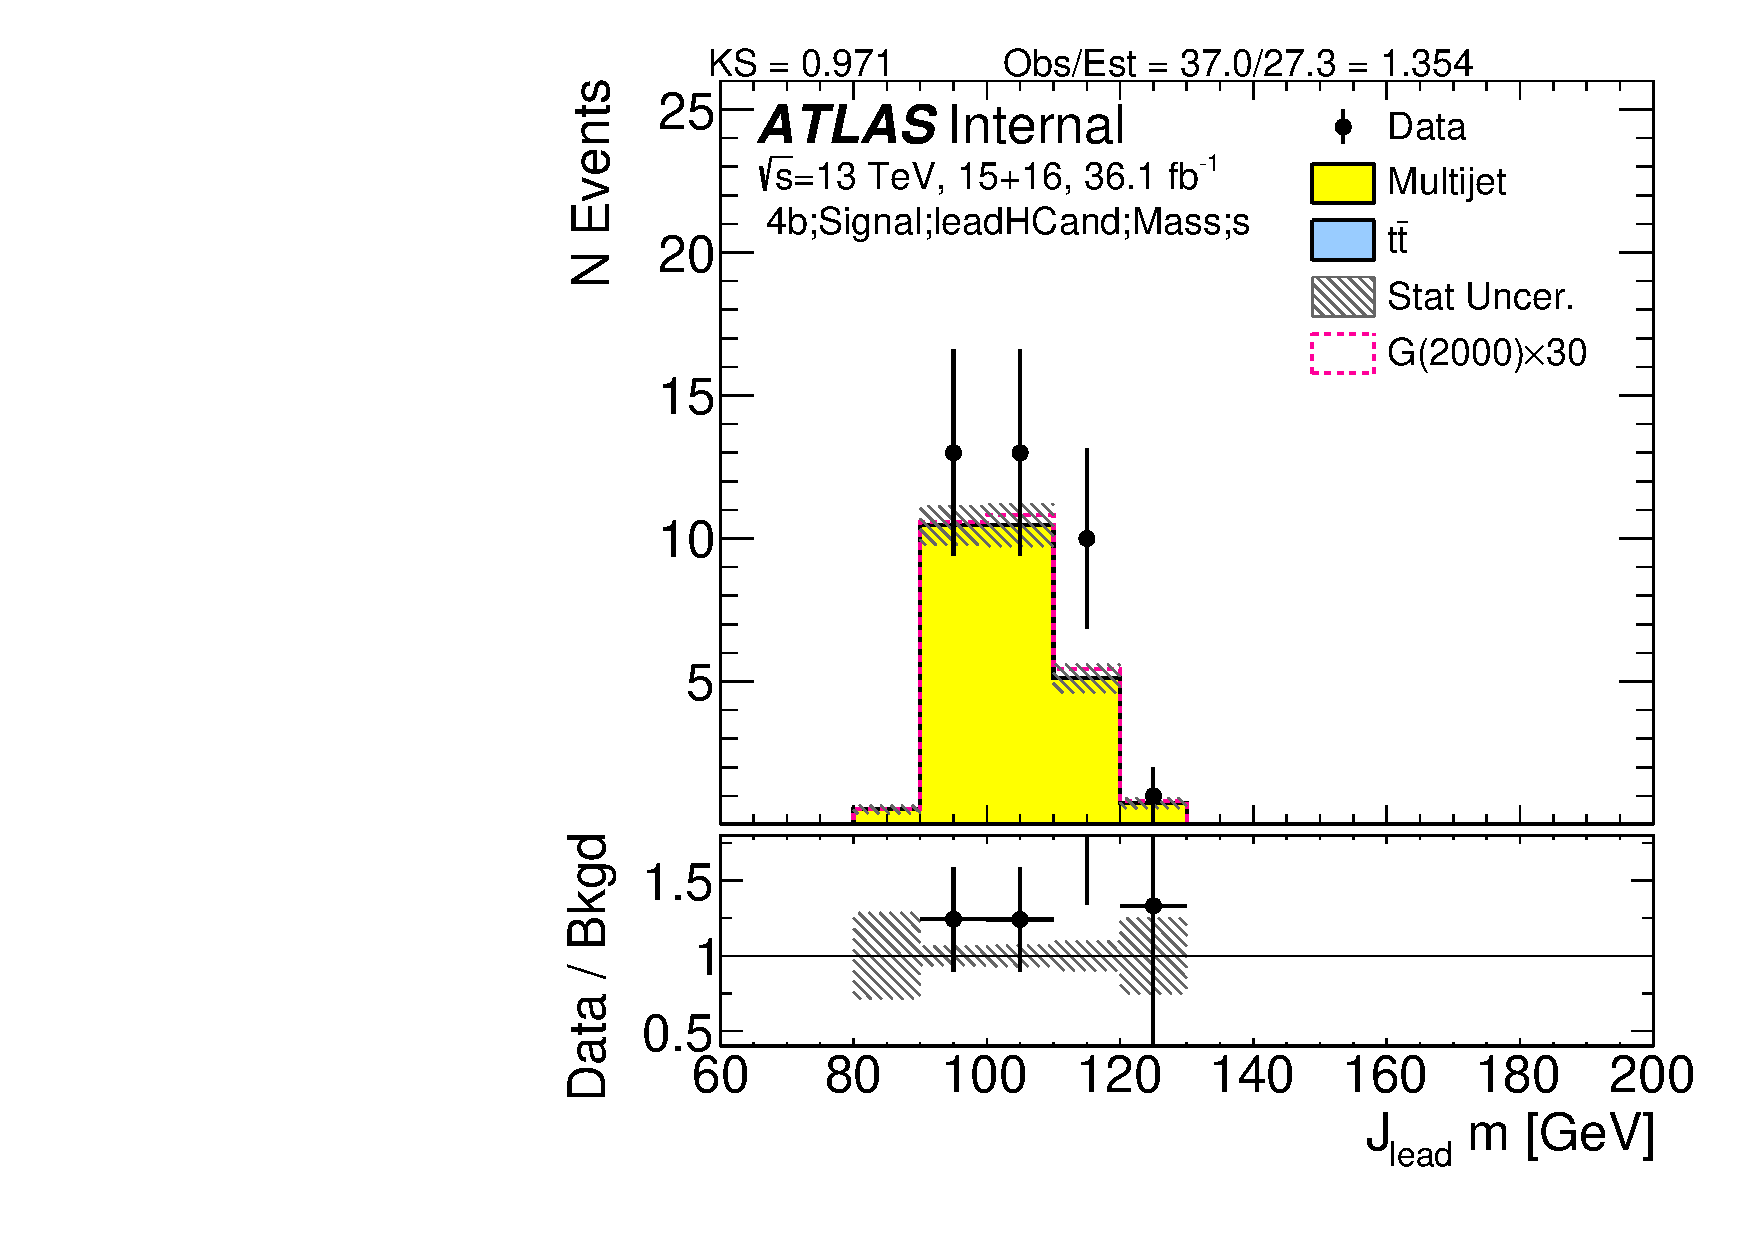
\includegraphics[width=0.45\textwidth,angle=-90]{figures/boosted/ZZ/Moriond_ZZ_FourTag_Signal_leadHCand_Mass_s.pdf}\\
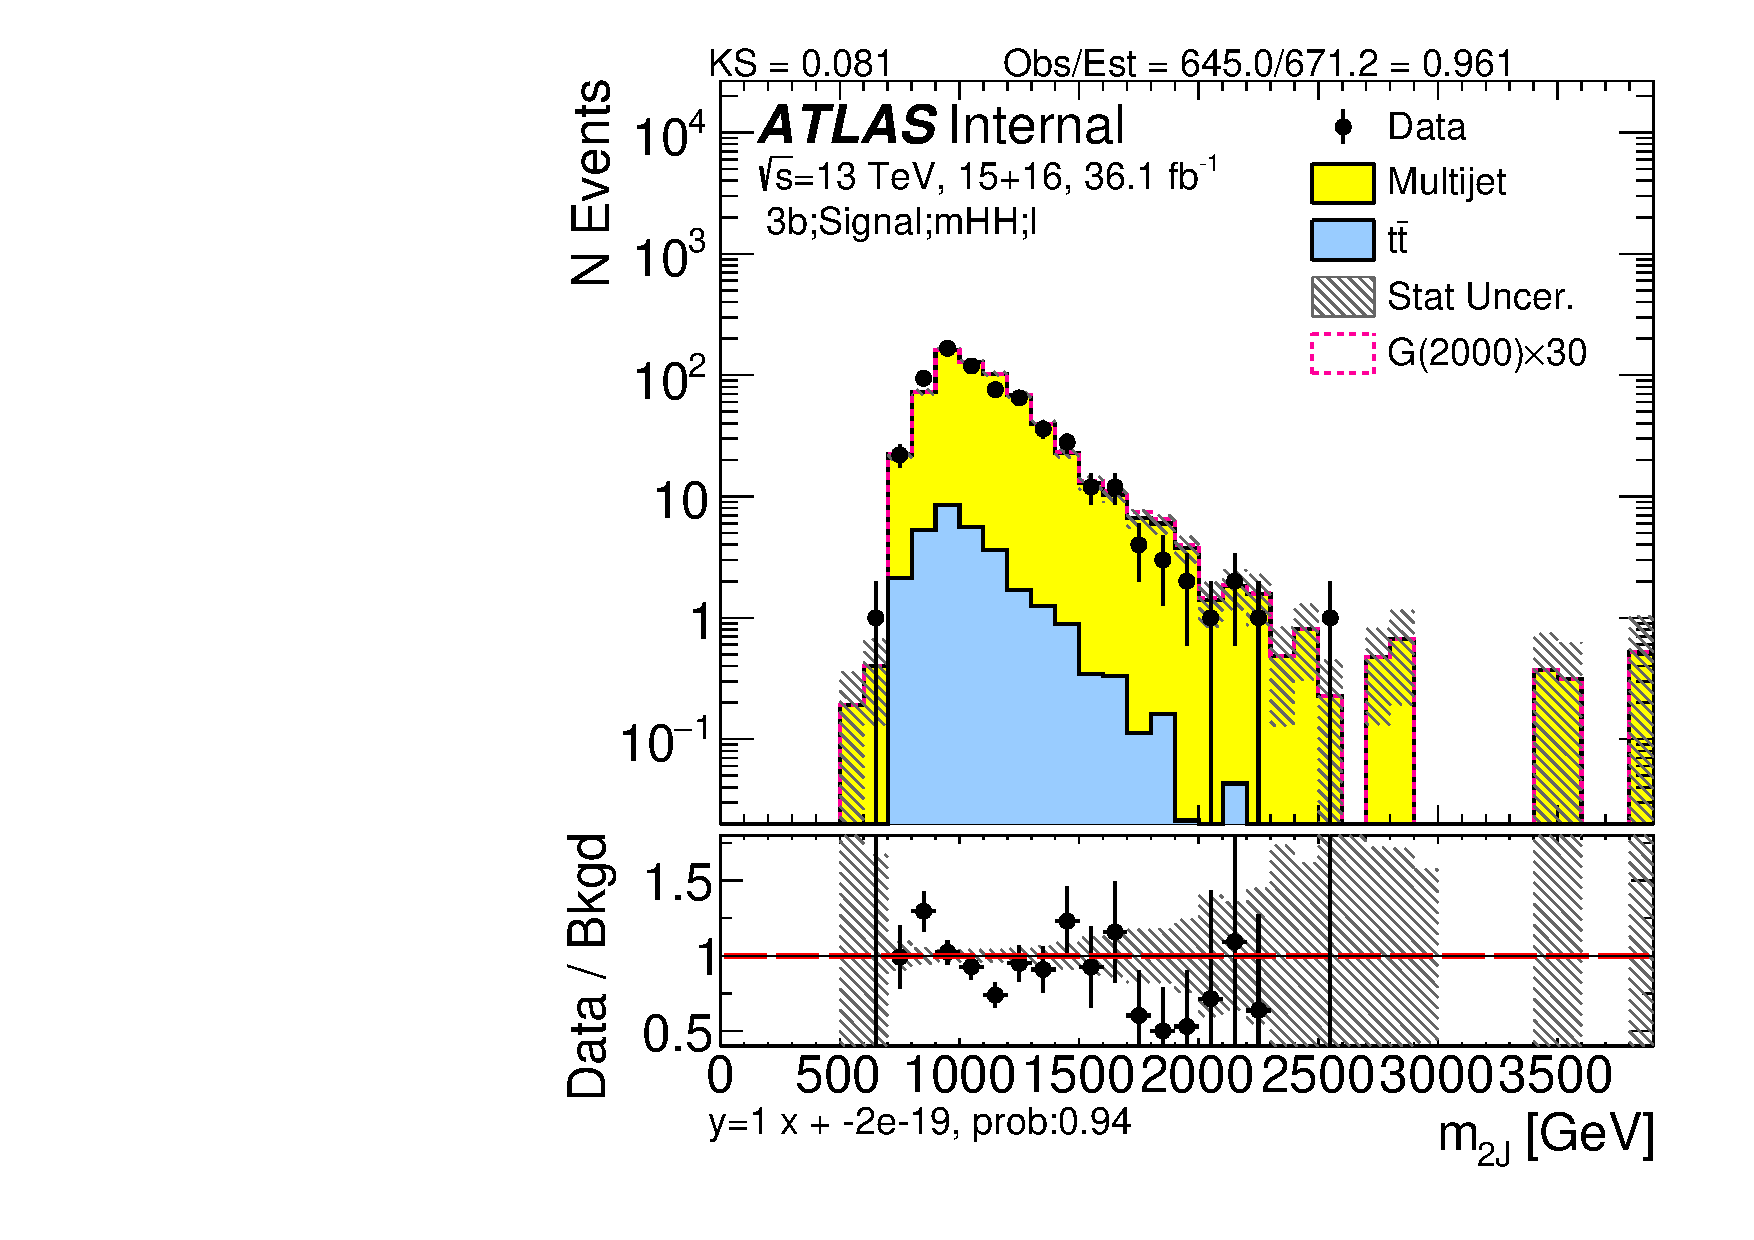
\includegraphics[width=0.45\textwidth,angle=-90]{figures/boosted/ZZ/Moriond_ZZ_ThreeTag_Signal_mHH_l_1.pdf}
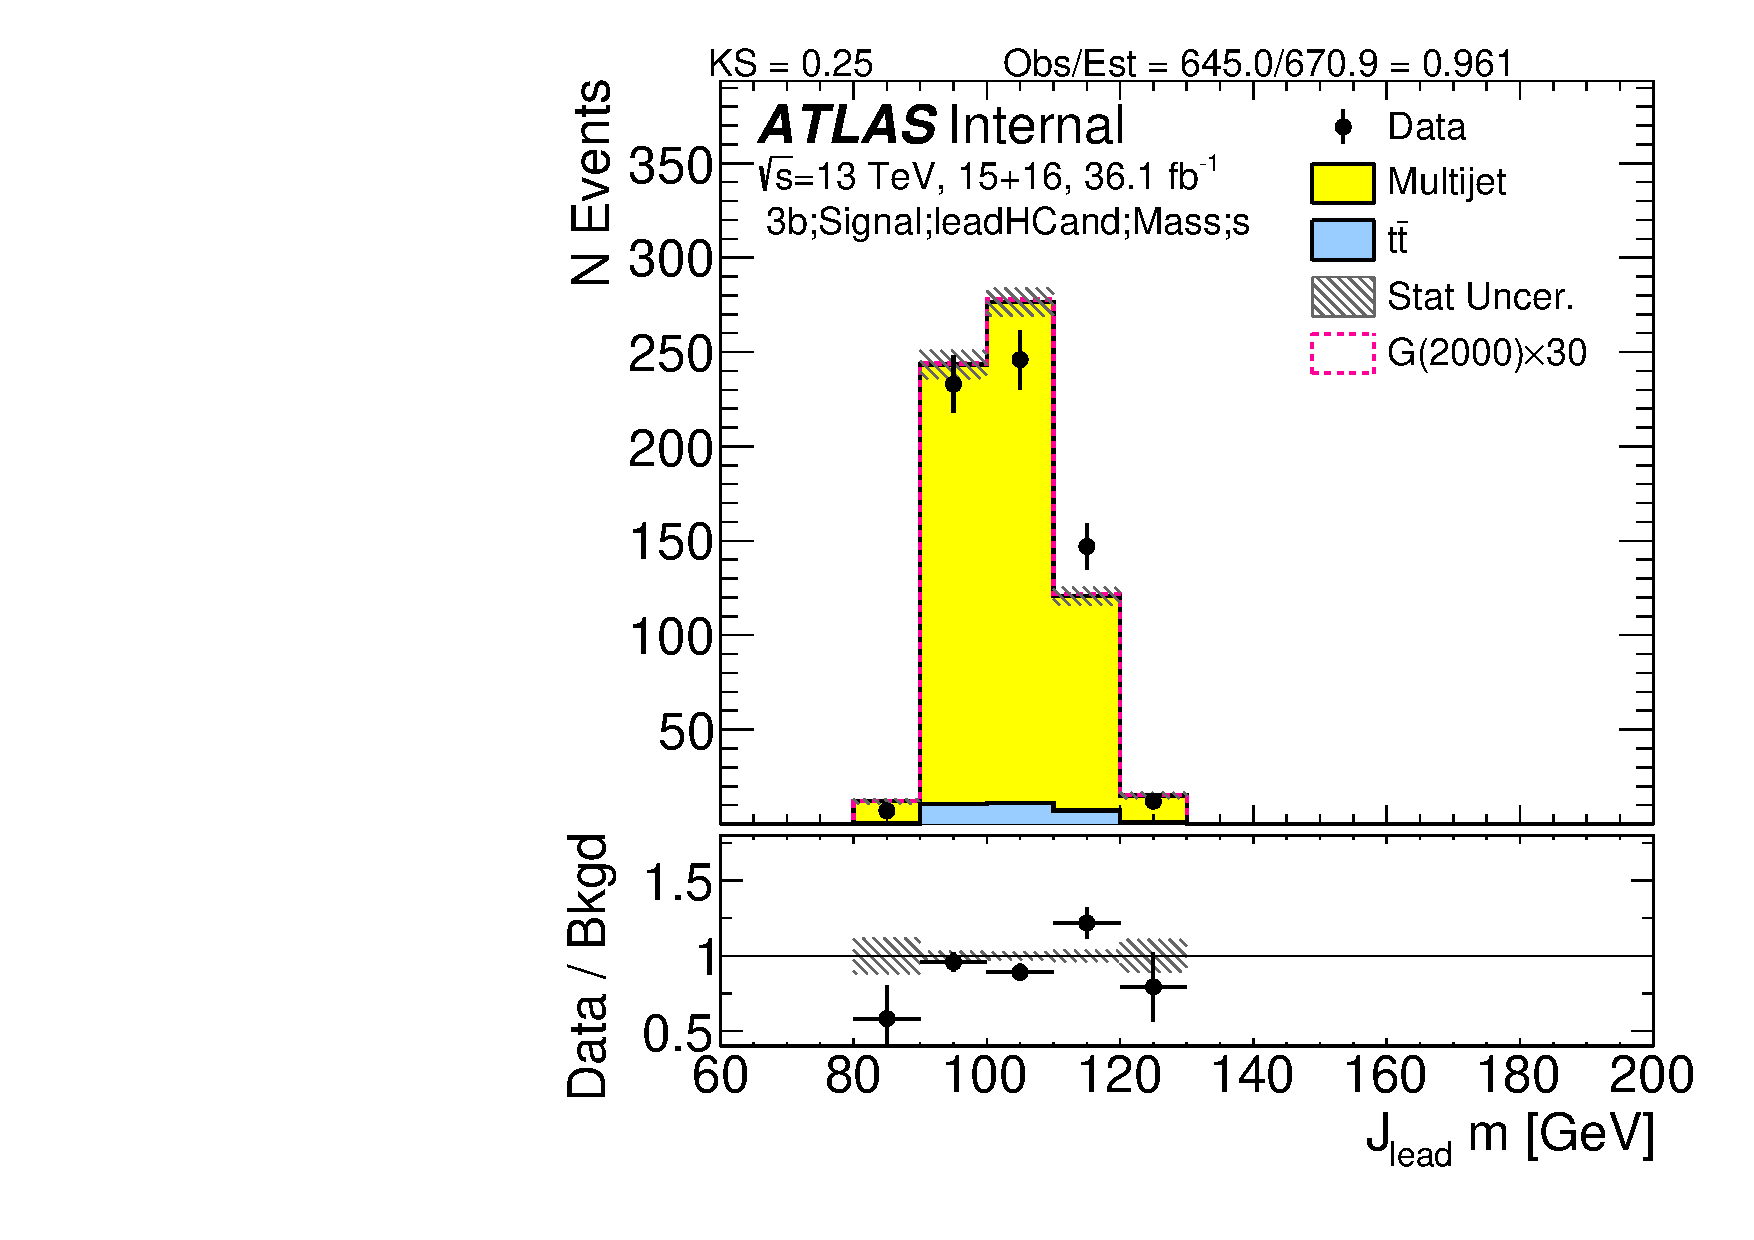
\includegraphics[width=0.45\textwidth,angle=-90]{figures/boosted/ZZ/Moriond_ZZ_ThreeTag_Signal_leadHCand_Mass_s.pdf}\\
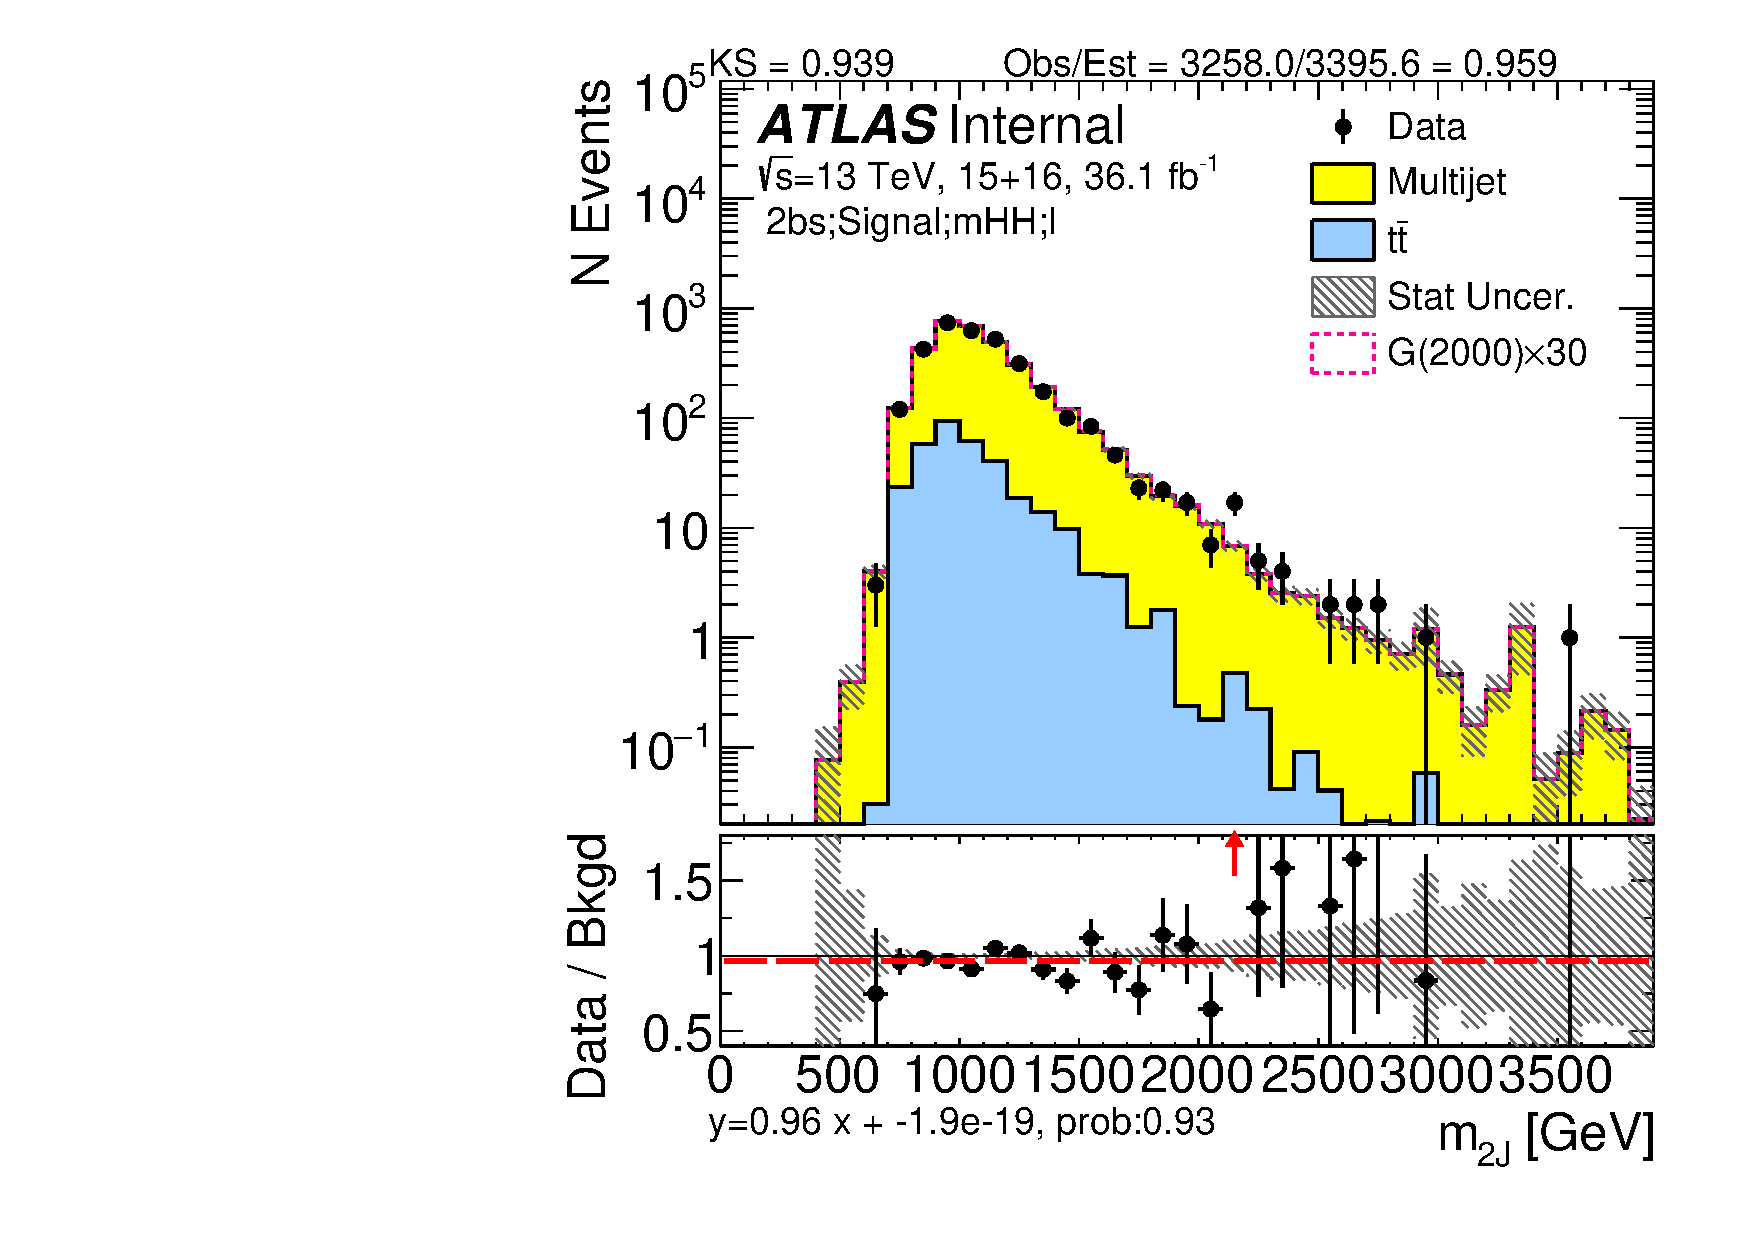
\includegraphics[width=0.45\textwidth,angle=-90]{figures/boosted/ZZ/Moriond_ZZ_TwoTag_split_Signal_mHH_l_1.pdf}
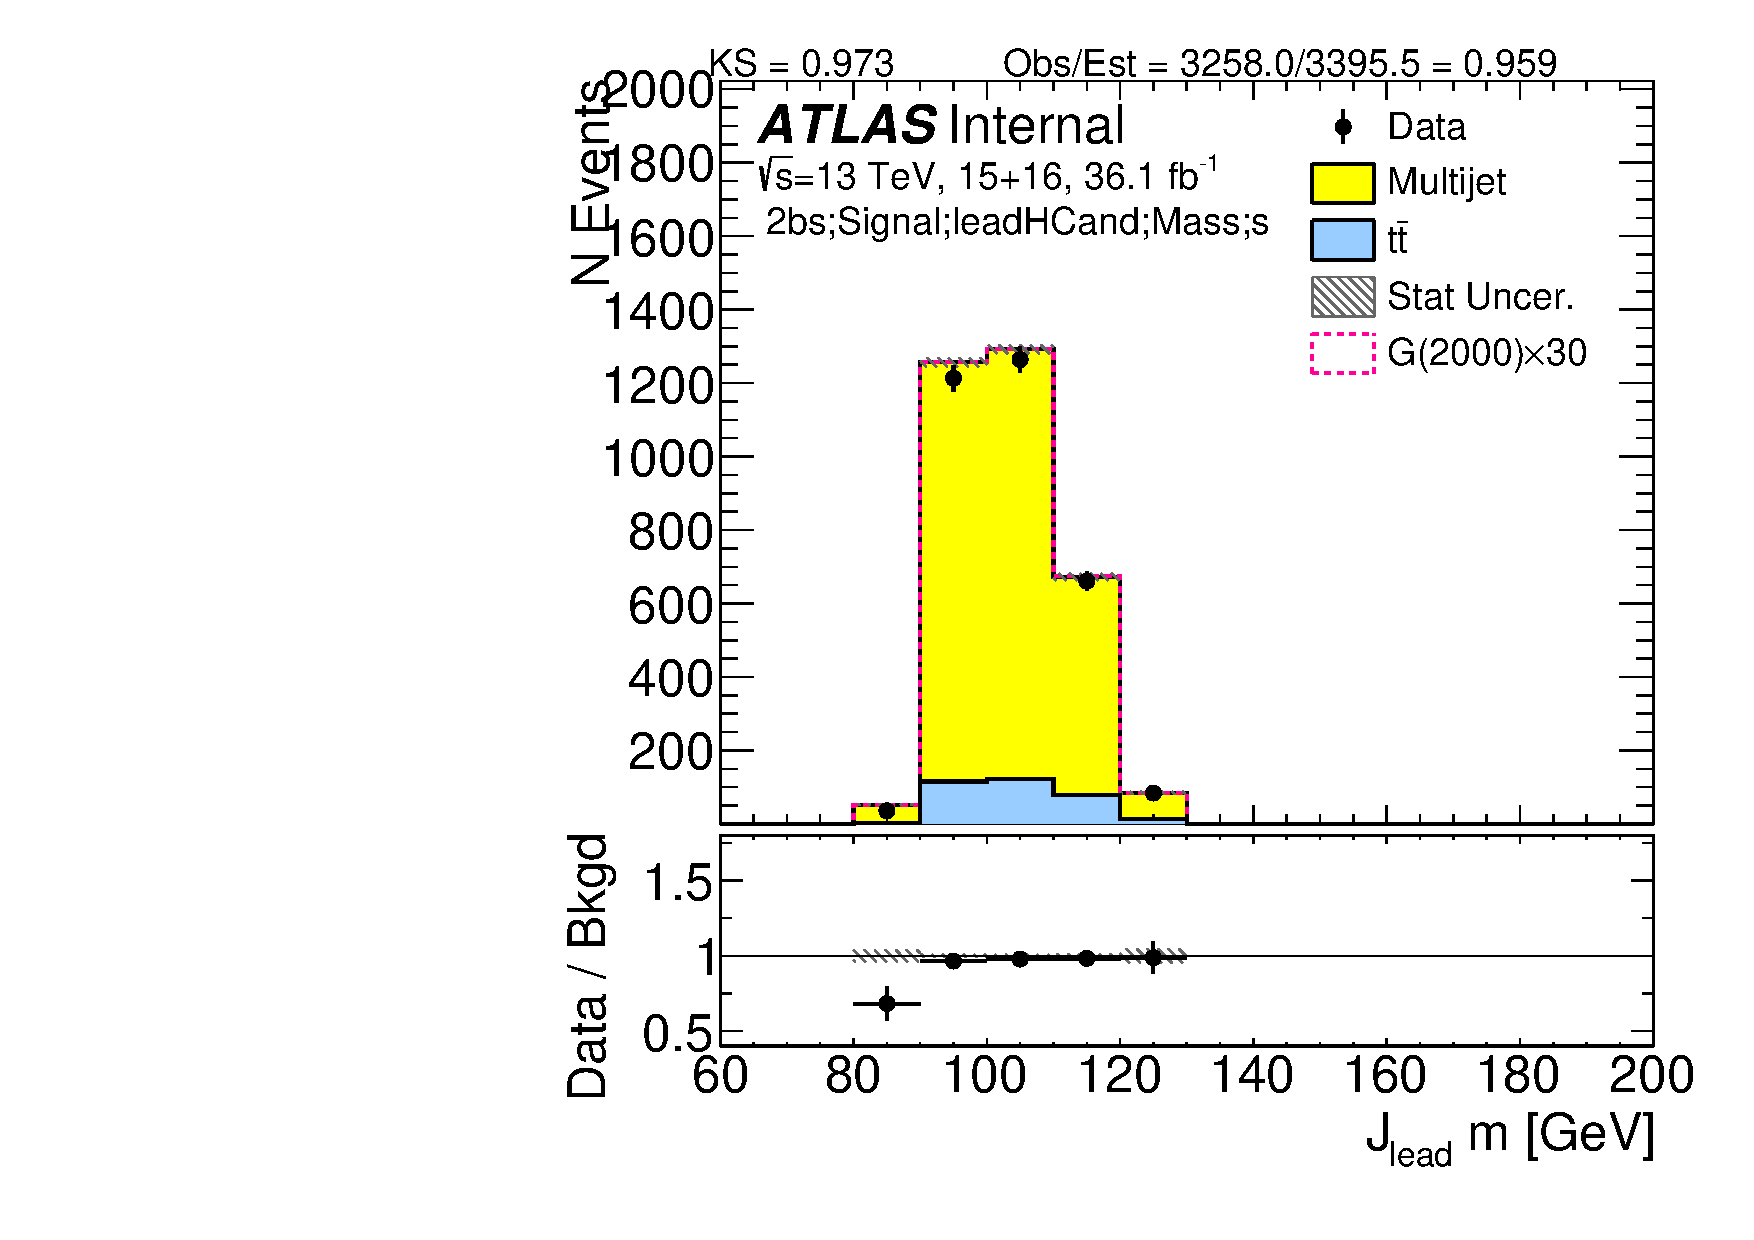
\includegraphics[width=0.45\textwidth,angle=-90]{figures/boosted/ZZ/Moriond_ZZ_TwoTag_split_Signal_leadHCand_Mass_s.pdf}\\
\end{center}
\caption{ZZ signal region distribution of \mtwoJ~ (left column) and leading large-R jet mass (right column) in low mass signal, for $4b$ (top row), $3b$(middle row) and $2b$ split (bottom row). The plots are with only statistical uncertainty.}
\label{CRSB:ZZSR_Distribution}
\end{figure}

% \begin{table}[htbp!]
% \begin{center}
% \begin{footnotesize} 
\begin{tabular}{c|c|c|c} 
FourTag & Sideband & Control & Signal \\ 
\hline\hline 
& & & \\ 
QCD Est & 152.28 $\pm$ 2.72 & 63.47 $\pm$ 1.77 & 28.6 $\pm$ 1.21\\ 
$t\bar{t}$ Est.  & 19.86 $\pm$ 0.22 & 7.45 $\pm$ 0.15 & 15.02 $\pm$ 0.2\\ 
$Z+jets$ & 0 $\pm$ 0 & 6.18 $\pm$ 5.12 & 0 $\pm$ 0\\ 
Total Bkg Est & 172.14 $\pm$ 2.73 & 77.1 $\pm$ 5.42 & 43.62 $\pm$ 1.23\\ 
Data & 172.0 $\pm$ 13.11 & 81.0 $\pm$ 9.0 & 46.0 $\pm$ 6.78\\ 
$c=1.0$,$m=1.0TeV$ & 2.38 $\pm$ 0.097 & 5.4 $\pm$ 0.15 & 0.15 $\pm$ 0.024\\ 
$c=1.0$,$m=2.0TeV$ & 0.033 $\pm$ 0.0015 & 0.1 $\pm$ 0.0026 & 0.0011 $\pm$ 0.00027\\ 
$c=1.0$,$m=3.0TeV$ & 0.00031 $\pm$ 3.6e-05 & 0.0008 $\pm$ 5.6e-05 & 1.5e-05 $\pm$ 7.7e-06\\ 
& & & \\ 
\hline\hline 
\end{tabular} 
\end{footnotesize} 
\newline 

% \end{center}
% \caption{Background prediction in SR/CR/SB for TT SR in $4b$-tag region. Uncertainties are stat only.}
% \label{CRSB:SummaryTable_TT_4b}
% \end{table}

% \begin{table}[htbp!]
% \begin{center}
% \begin{footnotesize} 
\begin{tabular}{c|c|c|c} 
ThreeTag & Sideband & Control & Signal \\ 
\hline\hline 
QCD Est & 3106.11 $\pm$ 25.79 & 1427.41 $\pm$ 17.53 & 570.01 $\pm$ 11.6\\ 
$t\bar{t}$ Est.  & 495.21 $\pm$ 18.75 & 148.55 $\pm$ 10.21 & 406.57 $\pm$ 5.42\\ 
$Z+jets$ & 32.5 $\pm$ 11.34 & 11.21 $\pm$ 5.65 & 0.3 $\pm$ 0.3\\ 
Total Bkg Est & 3633.82 $\pm$ 33.85 & 1587.17 $\pm$ 21.05 & 976.88 $\pm$ 12.81\\ 
Data & 3633.0 $\pm$ 60.27 & 1553.0 $\pm$ 39.41 & 1017.0 $\pm$ 31.89\\ 
$c=1.0$,$m=1.0TeV$ & 7.57 $\pm$ 0.18 & 12.58 $\pm$ 0.23 & 0.32 $\pm$ 0.037\\ 
$c=1.0$,$m=2.0TeV$ & 0.15 $\pm$ 0.0034 & 0.38 $\pm$ 0.0054 & 0.0047 $\pm$ 0.0006\\ 
$c=1.0$,$m=3.0TeV$ & 0.0034 $\pm$ 0.00012 & 0.0075 $\pm$ 0.00018 & 0.00023 $\pm$ 3.3e-05\\ 
\hline\hline 
\end{tabular} 
\end{footnotesize} 
\newline 

% \end{center}
% \caption{Background prediction in SR/CR/SB for TT SR in $3b$-tag region. Uncertainties are stat only.}
% \label{CRSB:SummaryTable_TT_3b}
% \end{table}

% \begin{table}[htbp!]
% \begin{center}
% \begin{footnotesize} 
\begin{tabular}{c|c|c|c} 
TwoTag split & Sideband & Control & Signal \\ 
\hline\hline 
QCD Est & 14980.05 $\pm$ 35.33 & 6803.06 $\pm$ 23.41 & 2817.92 $\pm$ 16.54\\ 
$t\bar{t}$ Est.  & 5170.92 $\pm$ 56.22 & 1468.85 $\pm$ 28.93 & 3628.91 $\pm$ 48.42\\ 
$Z+jets$ & 61.34 $\pm$ 16.04 & 26.44 $\pm$ 10.08 & 6.4 $\pm$ 5.05\\ 
Total Bkg Est & 20212.31 $\pm$ 68.31 & 8298.34 $\pm$ 38.56 & 6453.23 $\pm$ 51.41\\ 
Data & 20212.0 $\pm$ 142.17 & 8486.0 $\pm$ 92.12 & 6446.0 $\pm$ 80.29\\ 
$c=1.0$,$m=1.0TeV$ & 4.59 $\pm$ 0.14 & 6.33 $\pm$ 0.16 & 0.24 $\pm$ 0.033\\ 
$c=1.0$,$m=2.0TeV$ & 0.17 $\pm$ 0.0039 & 0.36 $\pm$ 0.0056 & 0.0066 $\pm$ 0.00077\\ 
$c=1.0$,$m=3.0TeV$ & 0.012 $\pm$ 0.00024 & 0.027 $\pm$ 0.00034 & 0.00089 $\pm$ 6.7e-05\\ 
\hline\hline 
\end{tabular} 
\end{footnotesize} 
\newline 

% \end{center}
% \caption{Background prediction in SR/CR/SB for TT SR in $2bs$-tag region. Uncertainties are stat only.}
% \label{CRSB:SummaryTable_TT_2b}
% \end{table}


\begin{figure}[htbp!]
\begin{center}
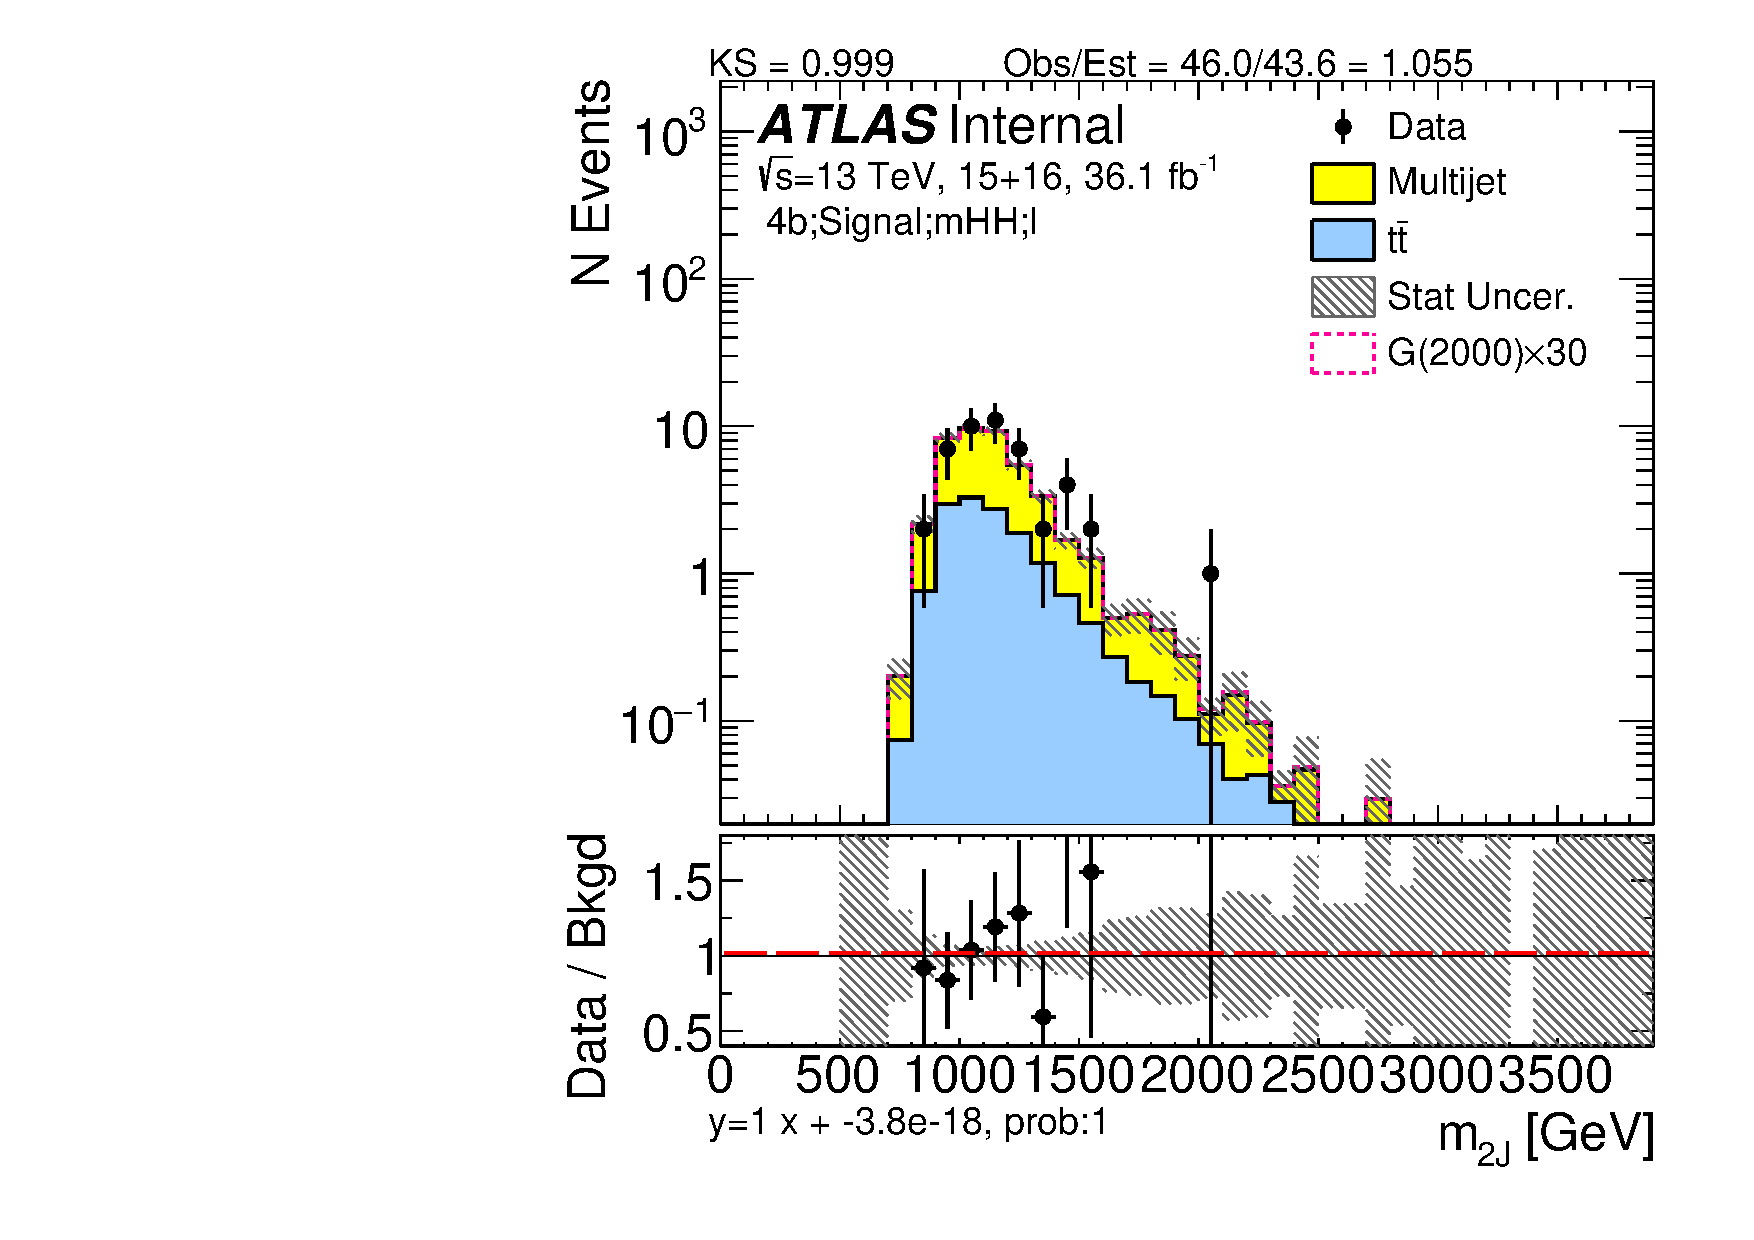
\includegraphics[width=0.45\textwidth,angle=-90]{figures/boosted/TT/Moriond_TT_FourTag_Signal_mHH_l_1.pdf}
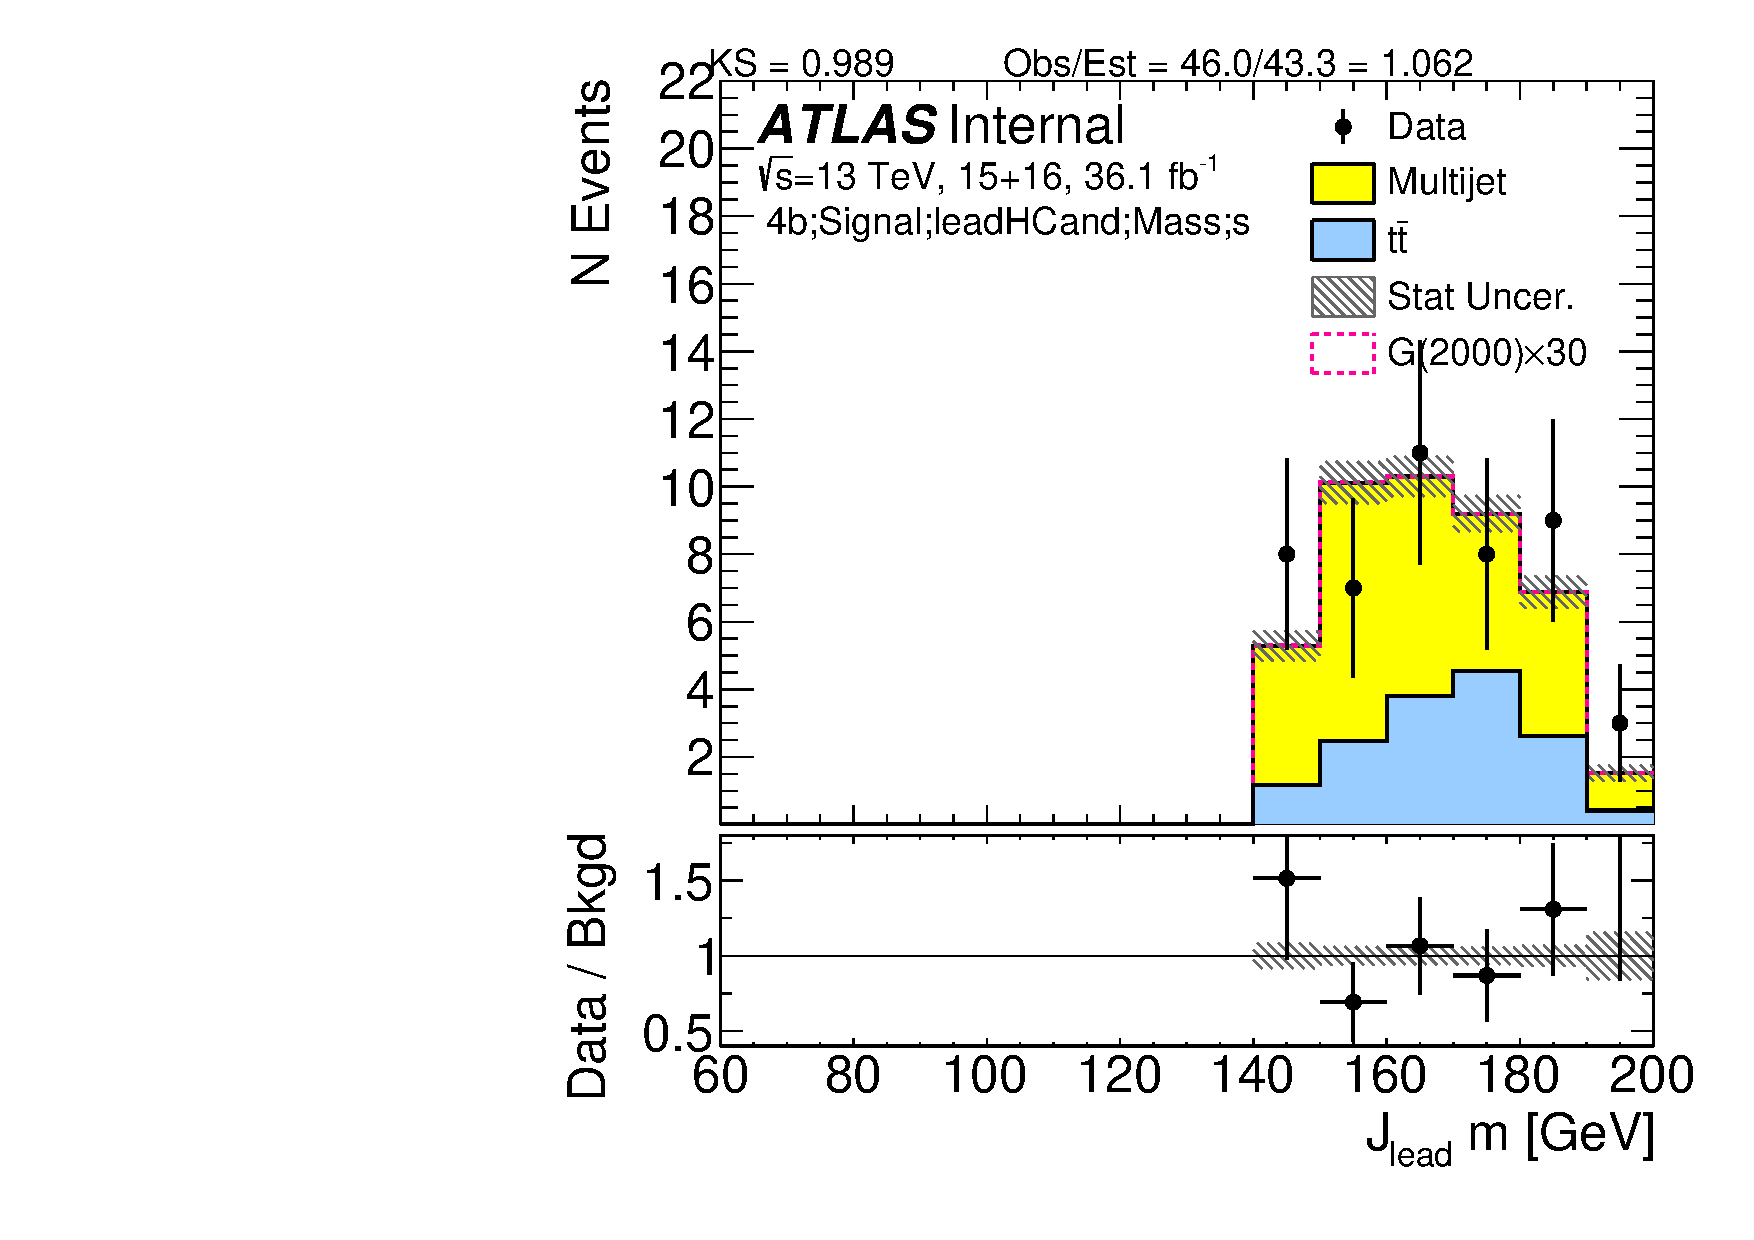
\includegraphics[width=0.45\textwidth,angle=-90]{figures/boosted/TT/Moriond_TT_FourTag_Signal_leadHCand_Mass_s.pdf}\\
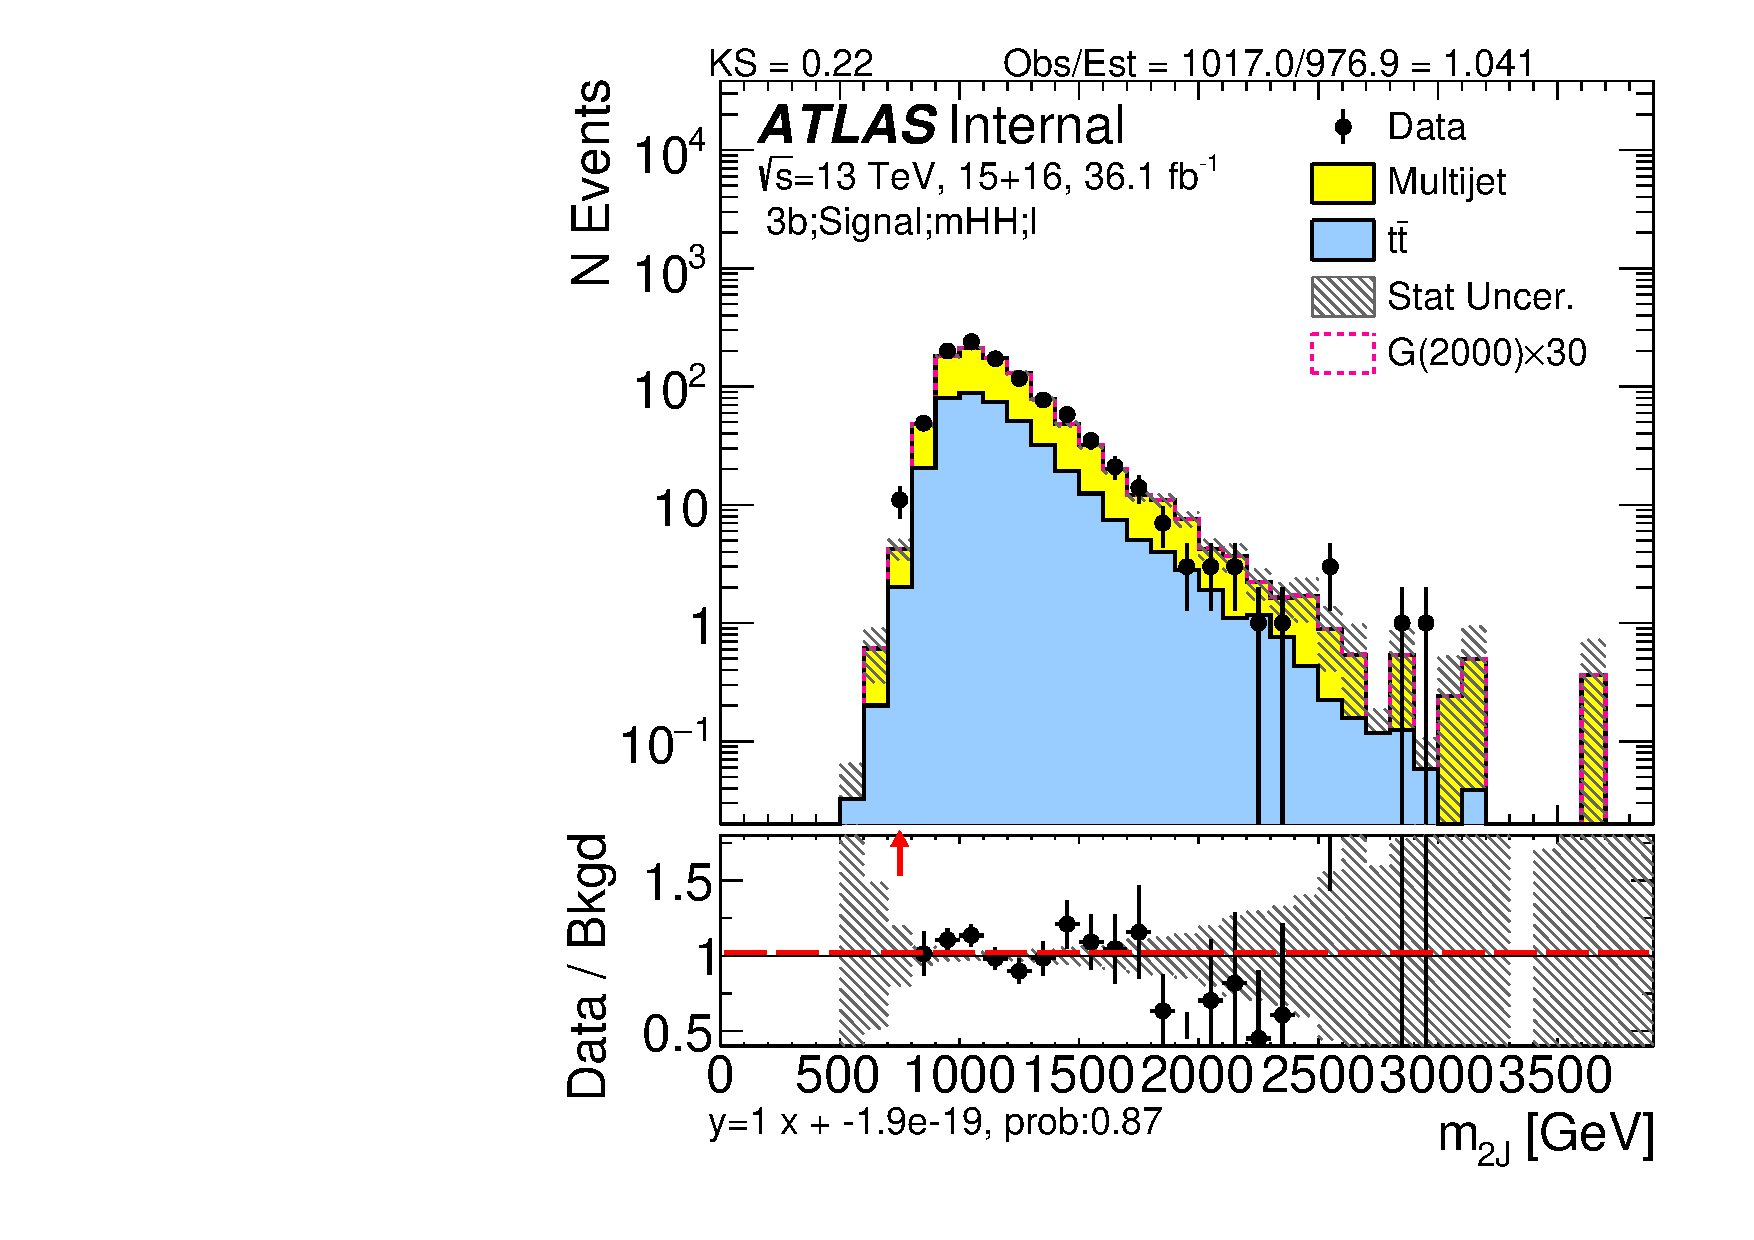
\includegraphics[width=0.45\textwidth,angle=-90]{figures/boosted/TT/Moriond_TT_ThreeTag_Signal_mHH_l_1.pdf}
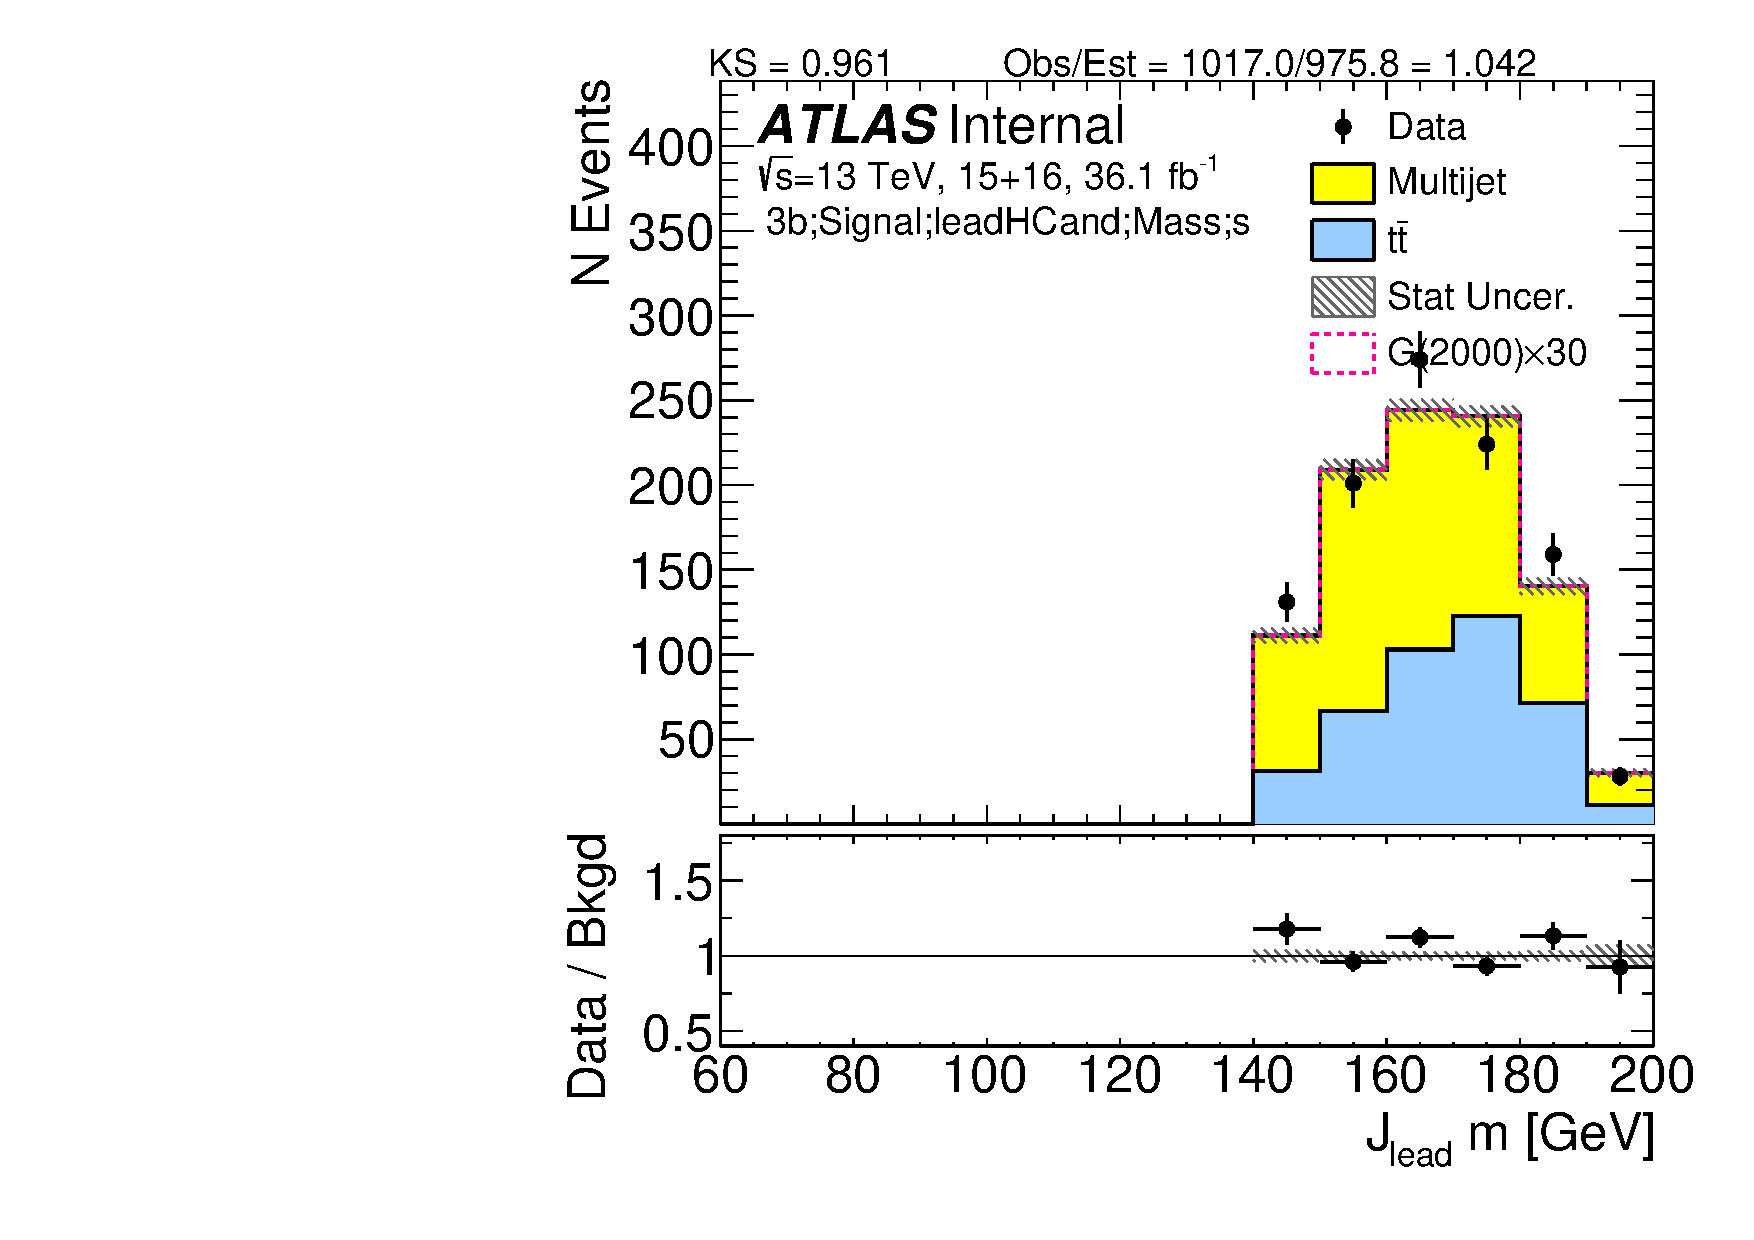
\includegraphics[width=0.45\textwidth,angle=-90]{figures/boosted/TT/Moriond_TT_ThreeTag_Signal_leadHCand_Mass_s.pdf}\\
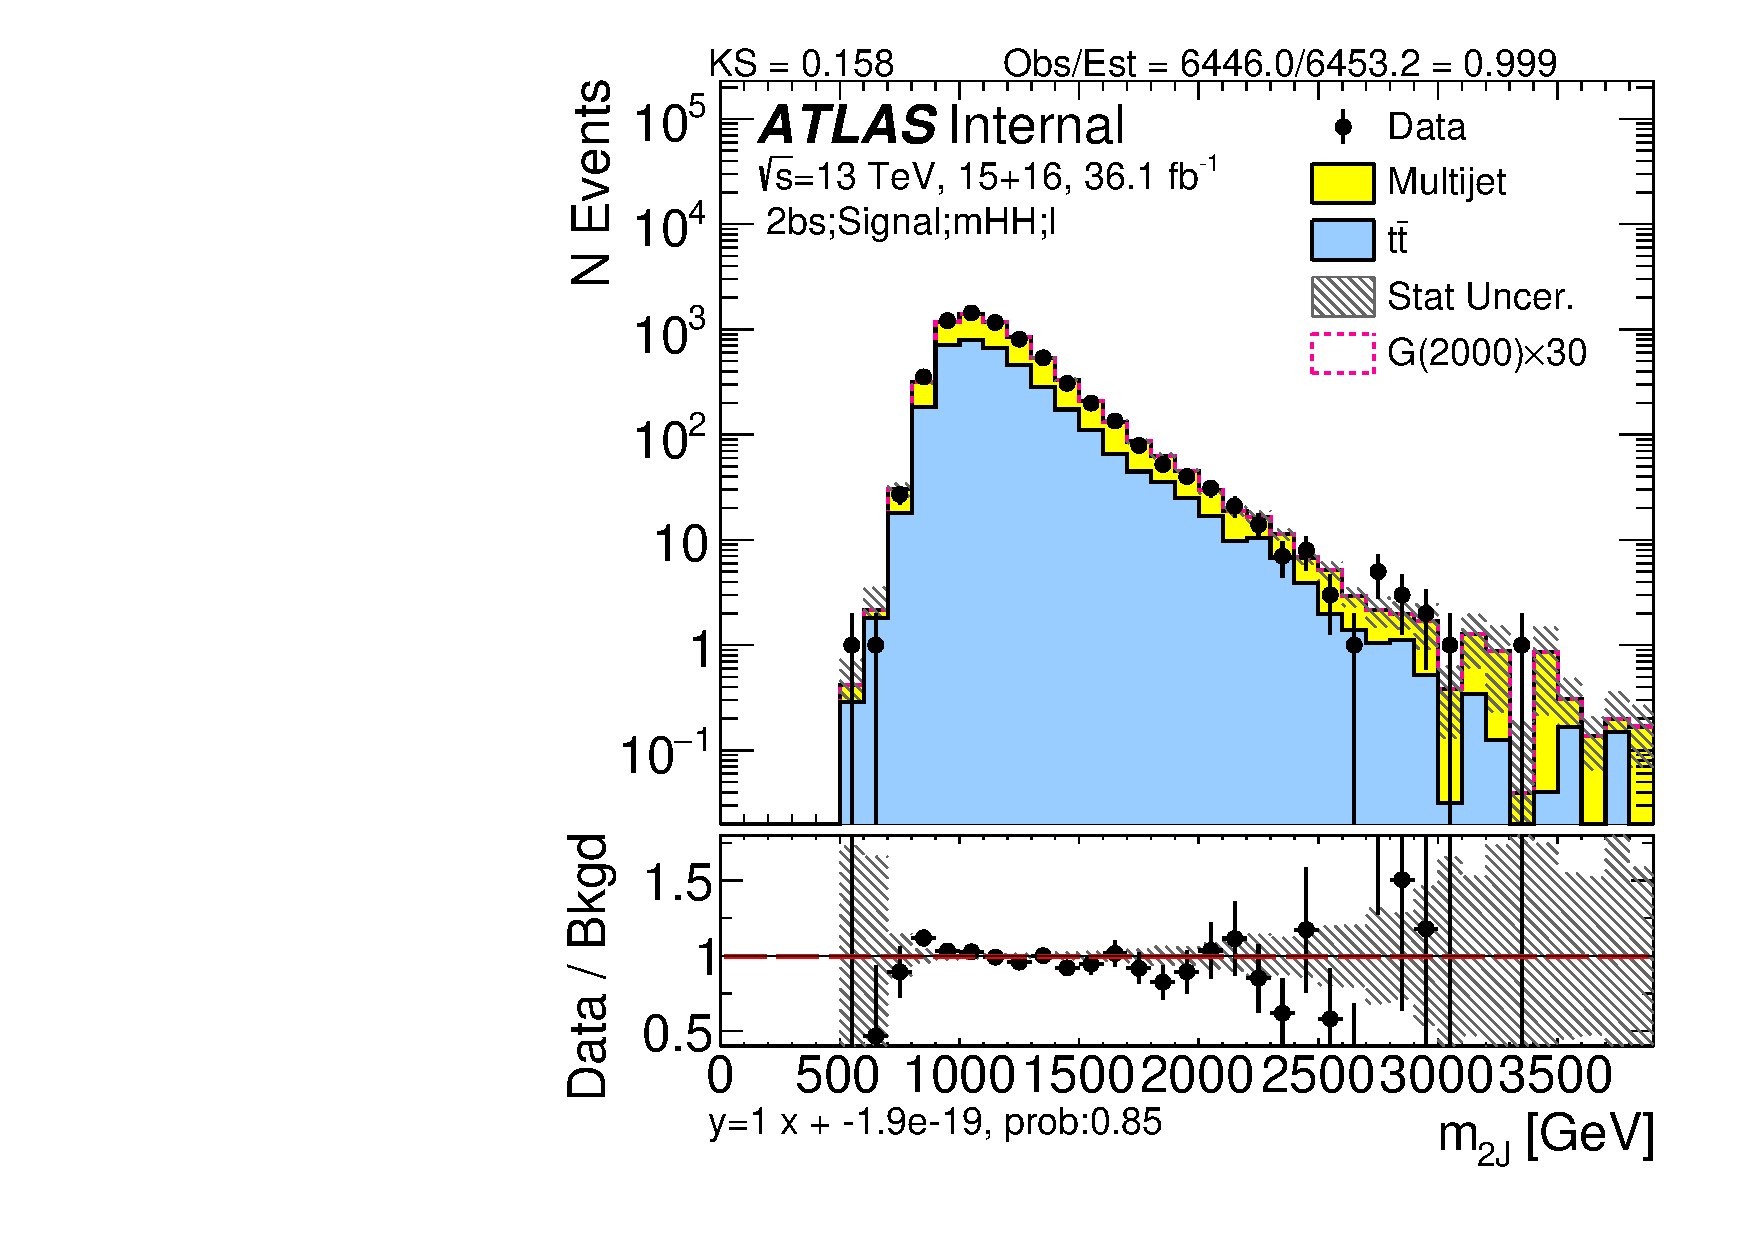
\includegraphics[width=0.45\textwidth,angle=-90]{figures/boosted/TT/Moriond_TT_TwoTag_split_Signal_mHH_l_1.pdf}
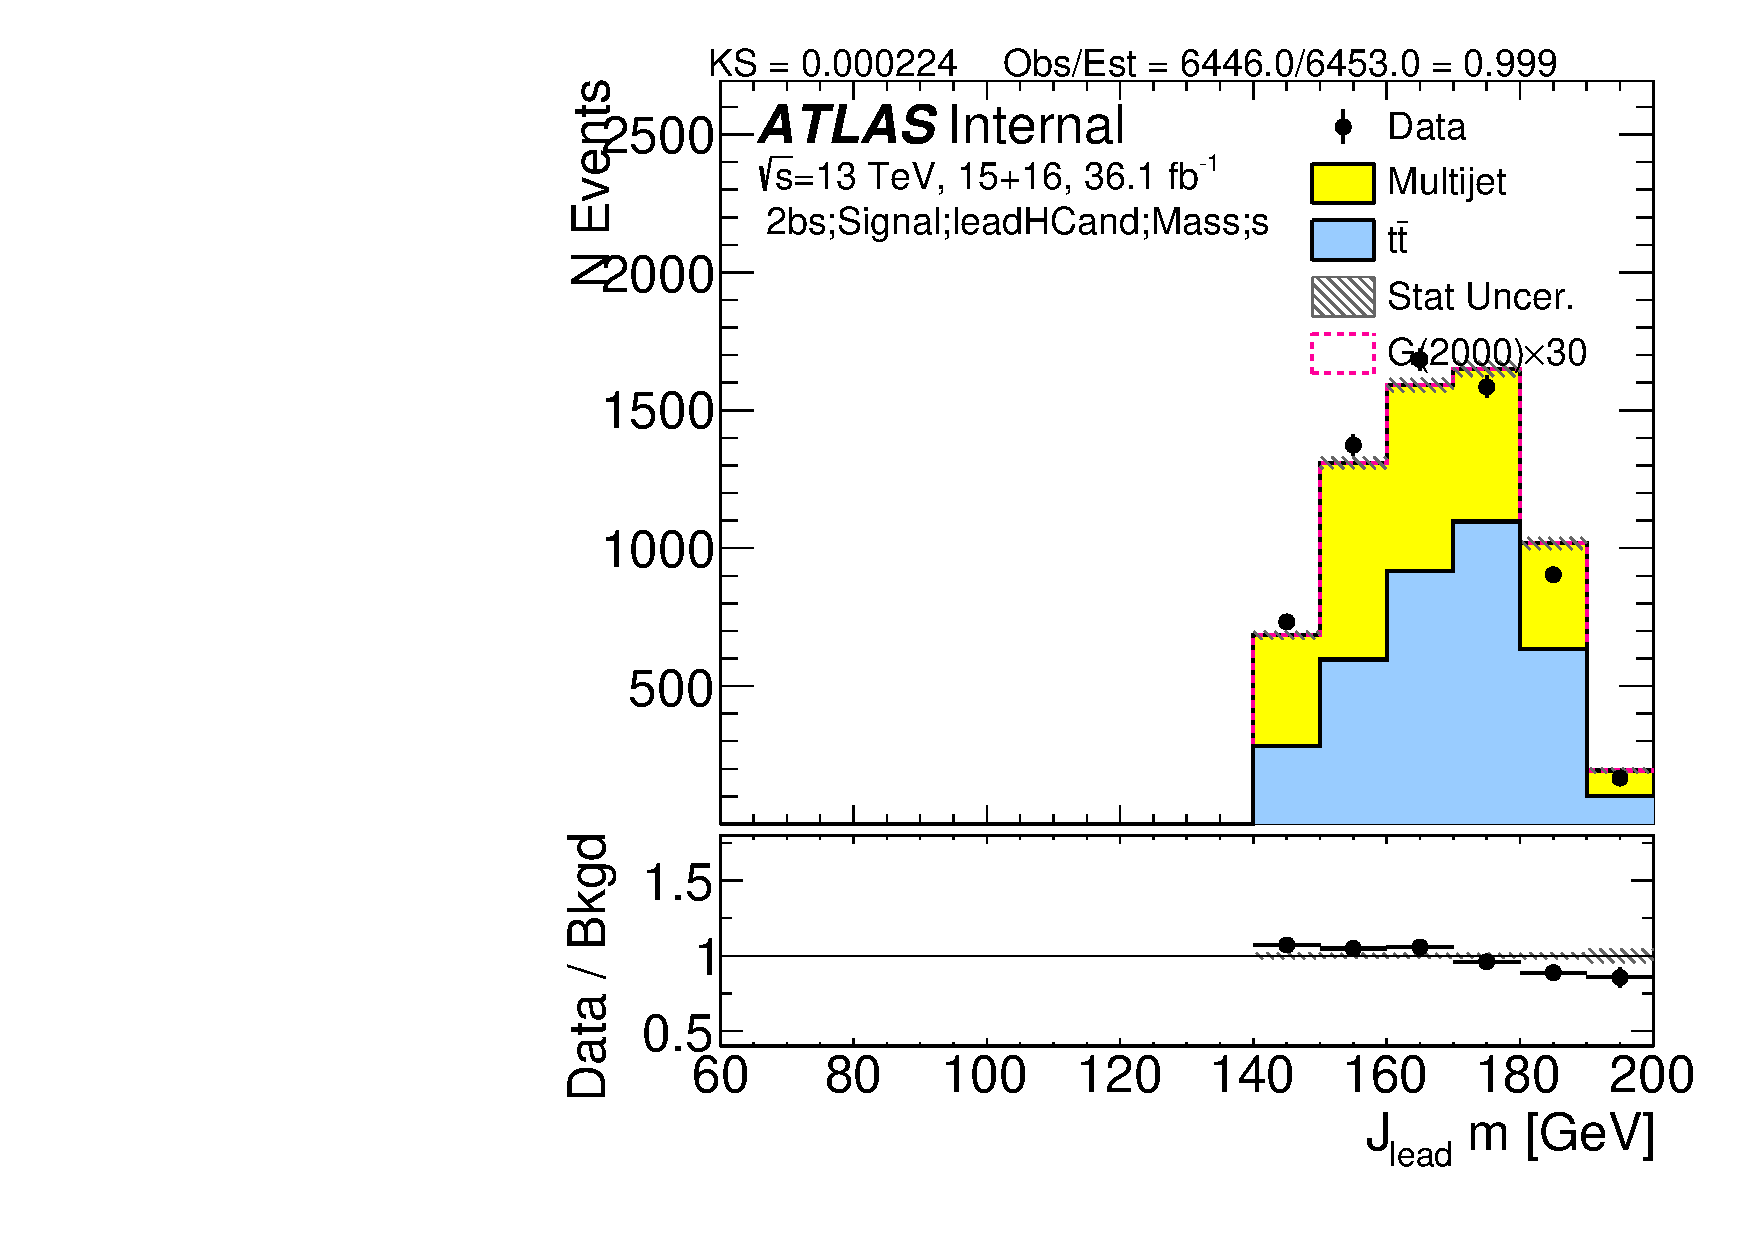
\includegraphics[width=0.45\textwidth,angle=-90]{figures/boosted/TT/Moriond_TT_TwoTag_split_Signal_leadHCand_Mass_s.pdf}\\
\end{center}
\caption{TT signal region distribution of \mtwoJ~ (left column) and leading large-R jet mass (right column) in low mass signal, for $4b$ (top row), $3b$(middle row) and $2b$ split (bottom row). The plots are with only statistical uncertainty.}
\label{CRSB:TTSR_Distribution}
\end{figure}


%%%%%%%%%%%%%%%%%%
\clearpage
\section{Uncertainty on the shape of \ttbar\ \mtwoJ~ in the $4/3b$ signal region}
\label{sec:unc-shape-ttbar-in-sr}

\paragraph{}
Because the $4/3b$ \ttbar\ \mtwoJ~ distribution is extremely statistically limited, the $2bs$ \ttbar\ \mtwoJ~ shape is used to predict the final \ttbar\ background shape in the $4/3b$ signal region.
In order to estimate the possible shape uncertainty, the $2bs$ and $3b$ sideband shapes are normalized and compared in Figure~\ref{fig:ttbar-shapes-signal}.  
In order to avoid large statistical uncertainties, the distributions of the $3b$ and $2b$ are smoothed. 
The ratio of the two smoothed distributions is taken as the shape systematic. 
This ratio is used to apply a bin-by-bin scaling of the \ttbar\ background prediction in the signal region, maintaining the same normalization given by nominal $t\bar{t}$ normalization prediction.

\begin{figure}[htbp!]
\begin{center} 
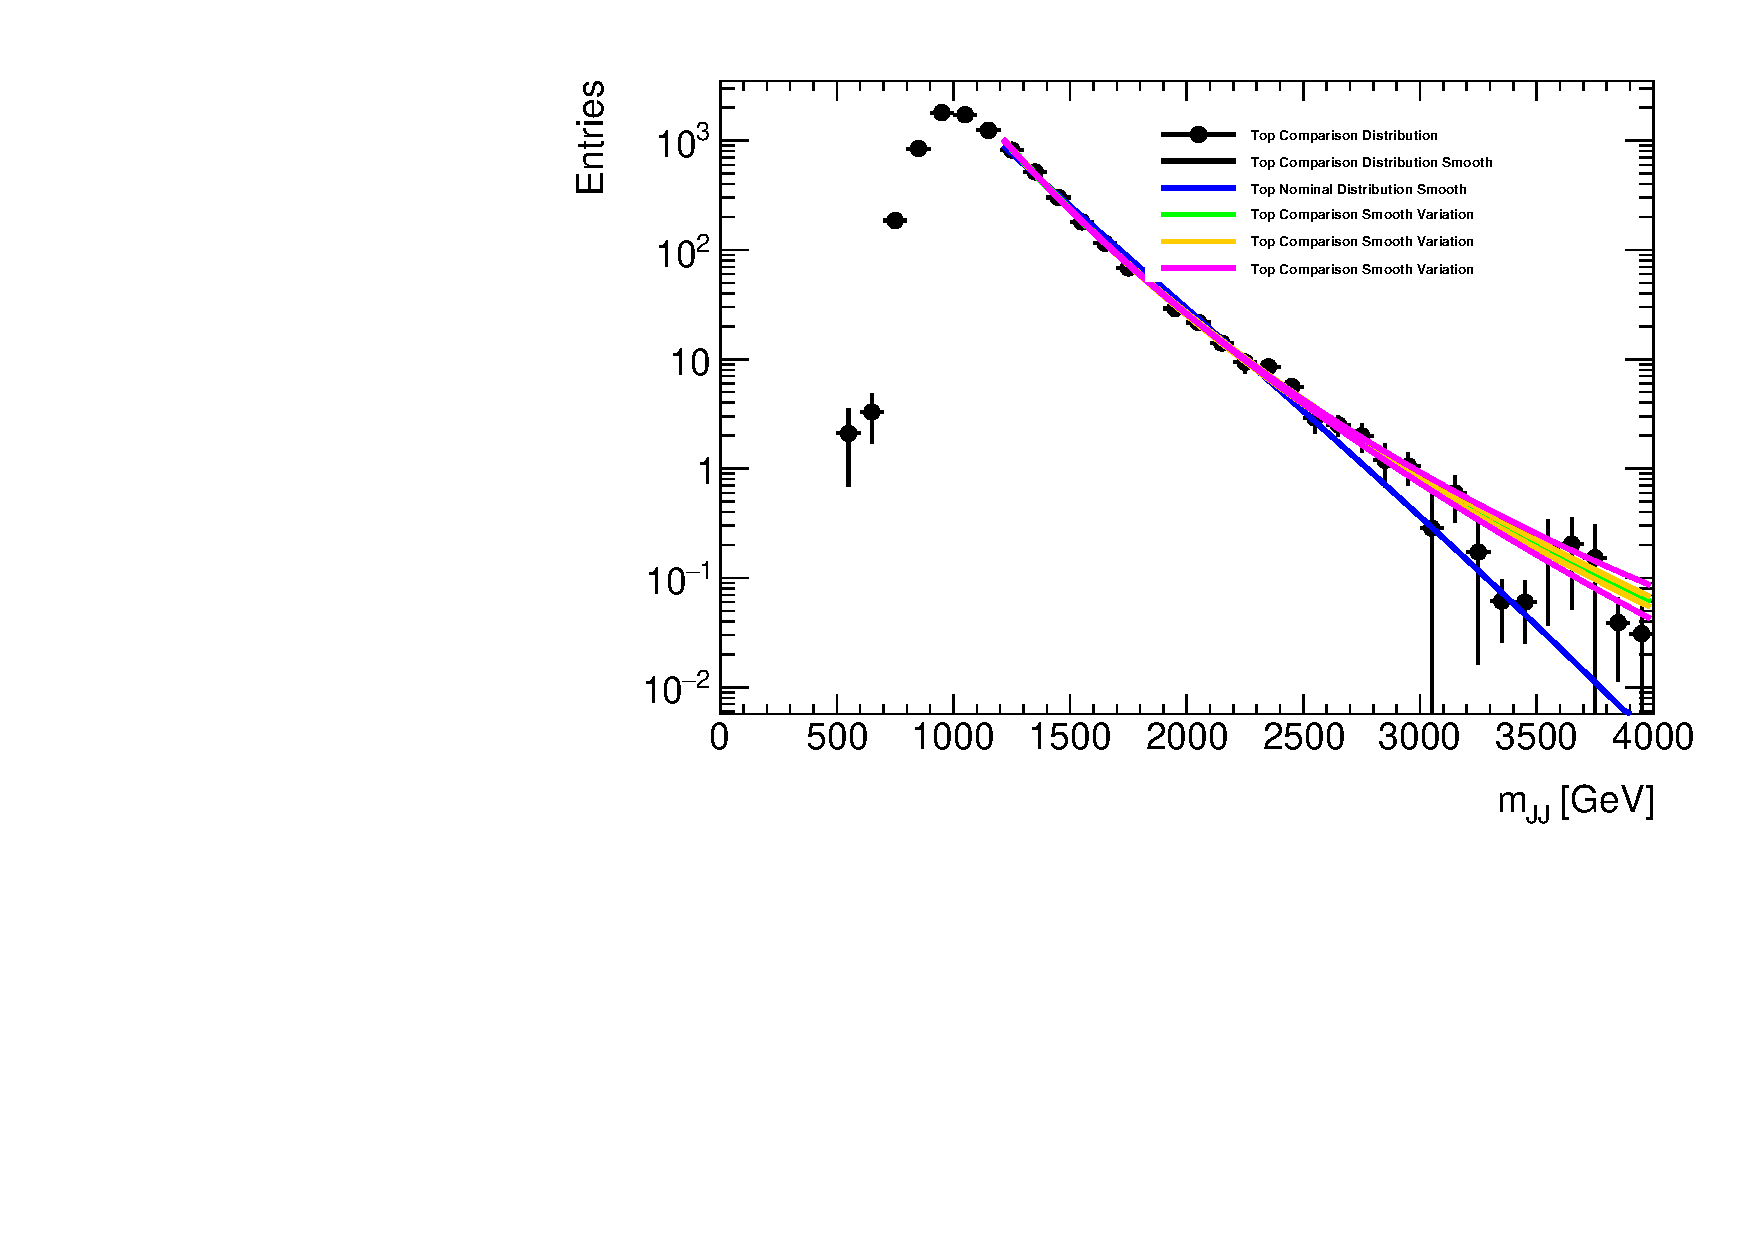
\includegraphics[width=0.31\textwidth,angle=-90]{figures/boosted/Syst_Smooth/TopShapeSRSysfitSmooth_sig33_comp22.pdf}
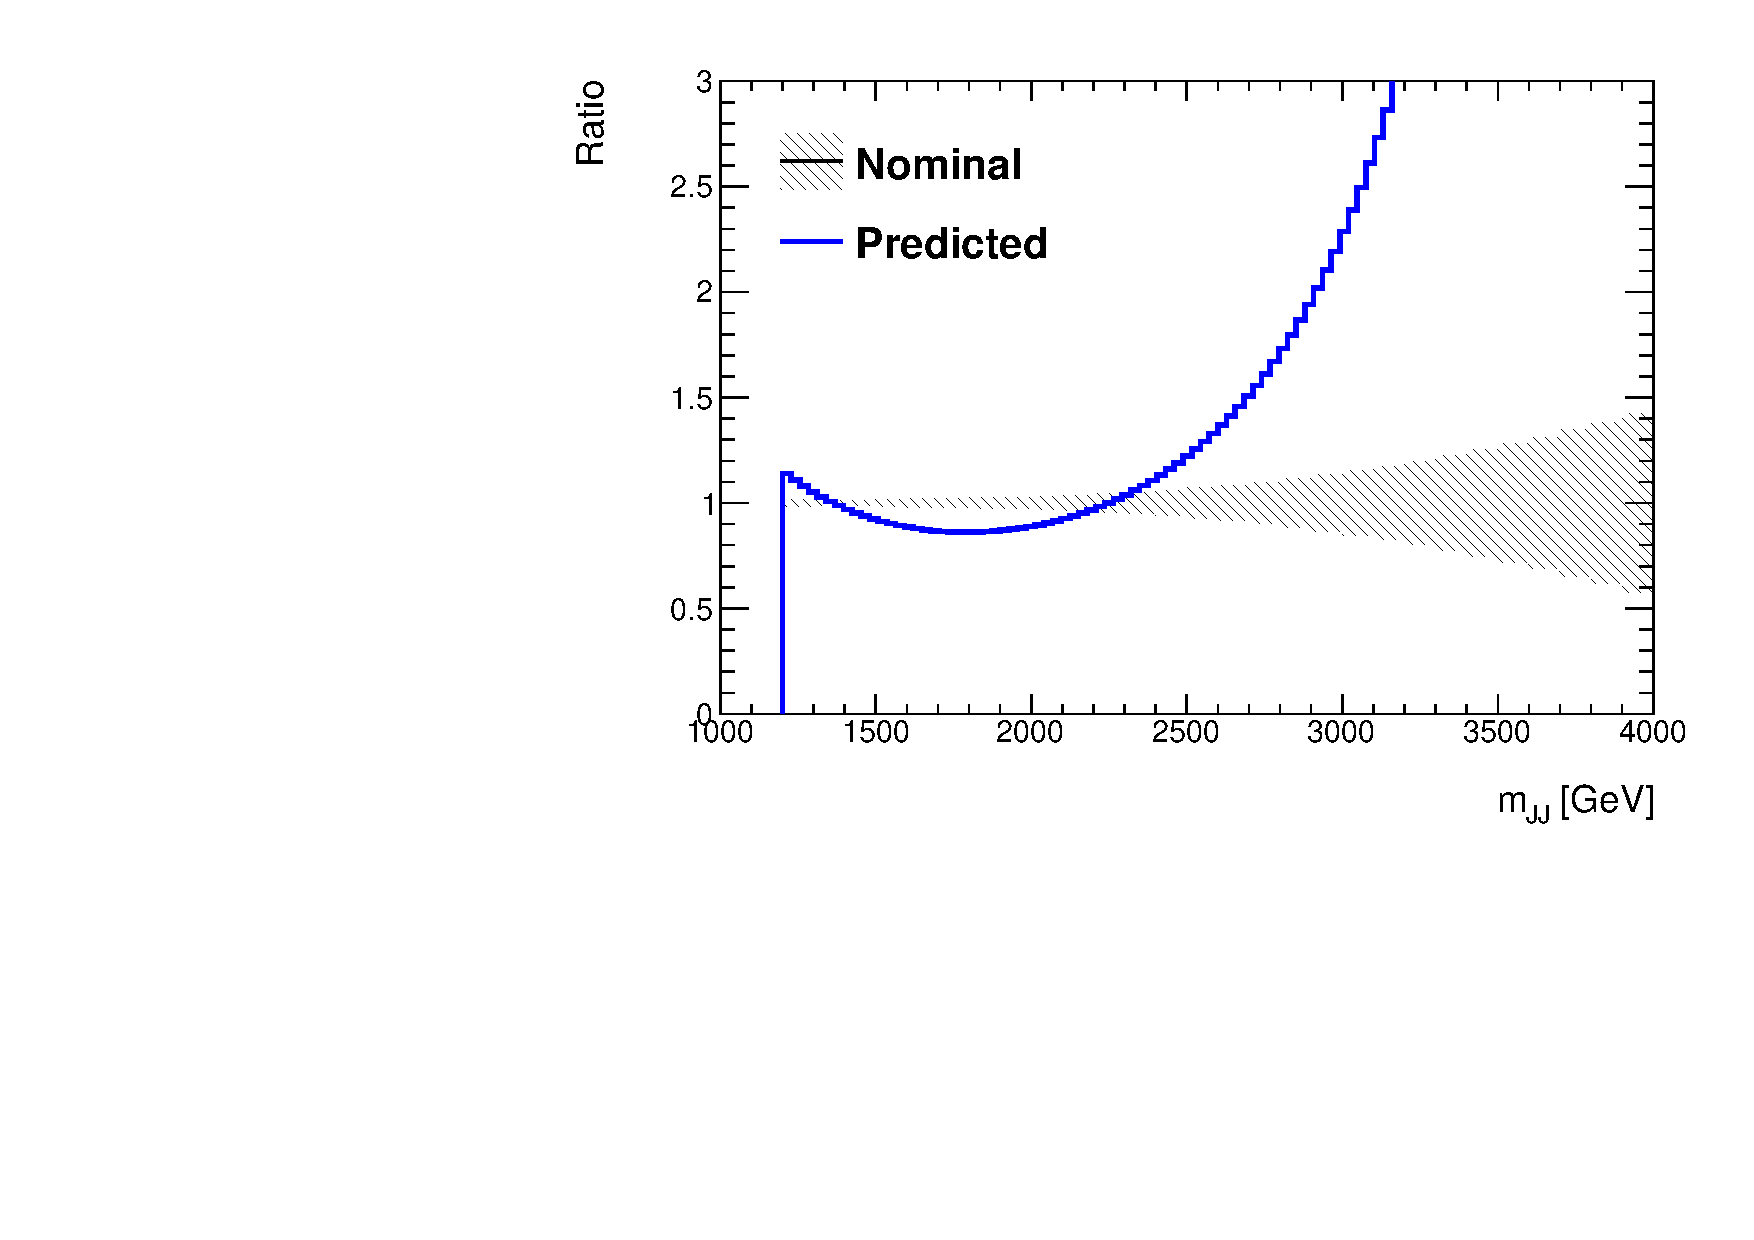
\includegraphics[width=0.31\textwidth,angle=-90]{figures/boosted/Syst_Smooth/TopShapeSRSysfitSmooth_sig33_comp22_ratio.pdf}
\caption{The shape of \ttbar~ \mtwoJ~ in the sideband region,
comparing the $3b$ shape with that of the $2bs$, in order to asses the systematic effect of additional $b$-tags changing the dijet mass distribution.  The \mtwoJ~ distributions is shown on the left, and the ratio of $3b$ to $2bs$ distributions on the right.}
\label{fig:ttbar-shapes-signal}
\end{center}
\end{figure}


\section{Uncertainty on the shape of the QCD distribution in the signal region}
\label{unc-shape-qcd-in-sr}

\paragraph{}
As shown in Figures~\ref{fig:boosted-cr-mjj}, the shape of the total predicted background distribution is found to be in good agreement with the $4b$, $3b$, and $2bs$ data in the control region. 
However due to the low statistics in the high \mtwoJ mass bins, there are statistical fluctuations that cannot be ignored. 
A comparison is performed by first smoothing the prediction and the data distribution in the control region. 
The ratio of the smoothed QCD distributions to that of the smoothed $4/3/2bs$ data distributions is taken as the shape systematic. 
This ratio is then used to apply a bin-by-bin scaling of the QCD background prediction in the signal region, maintaining the same normalization given by \muqcd.  
The smoothing fit and the ratios can be found in Figure~\ref{fig:qcd_shape_fit}. 
This systematics is further split into two parts: one below $2000$ \GeV~ and the other above $2000$ \GeV~, to ensure the low and high mass shape variation post-fit pulls can vary independently.
This uncertainty is applied for both the \mtwoJ, and the scaled \mtwoJ~ distribution, since the scaling correction has small impacts on \mtwoJ. 

\begin{figure}[htbp!]
\begin{center}
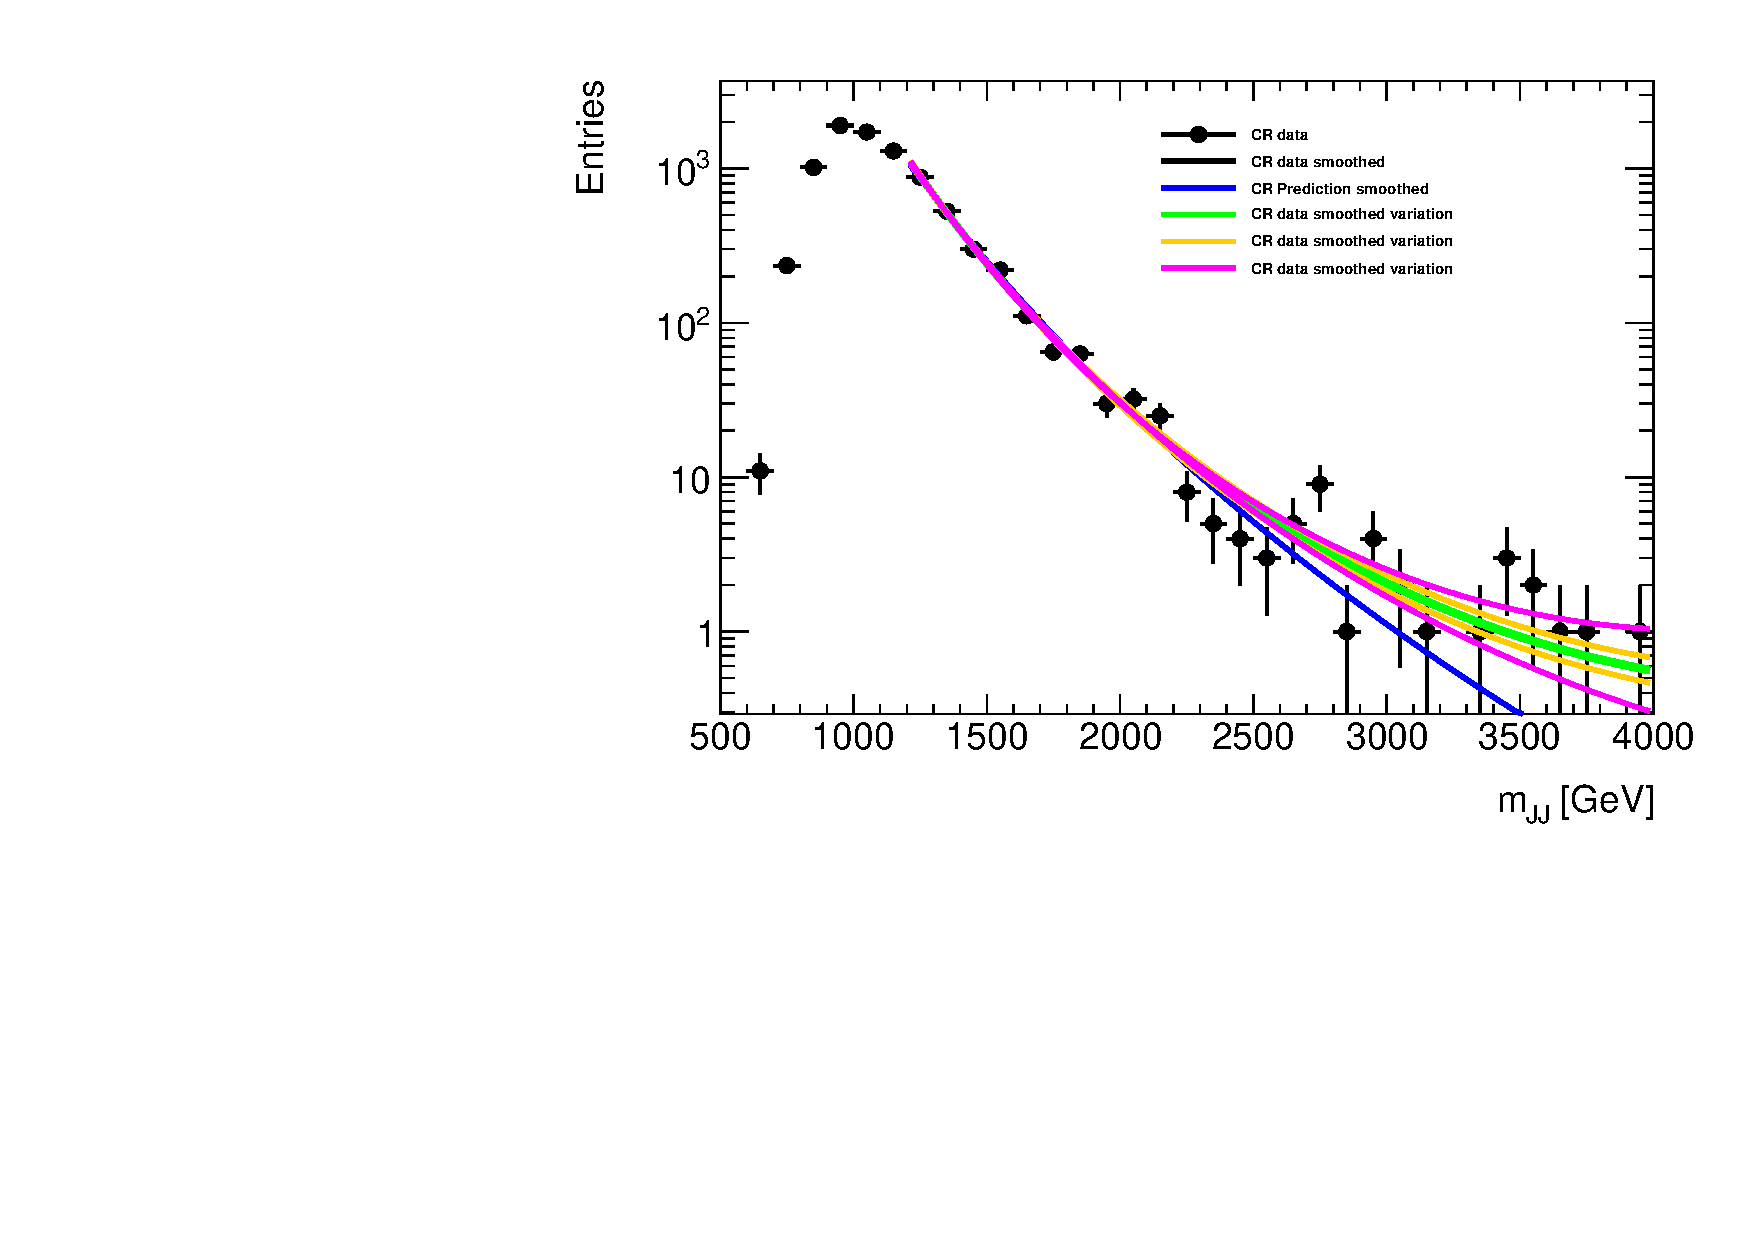
\includegraphics[width=0.31\textwidth,angle=-90]{figures/boosted/Syst_Shape/QCDSysfitSmooth_22.pdf}
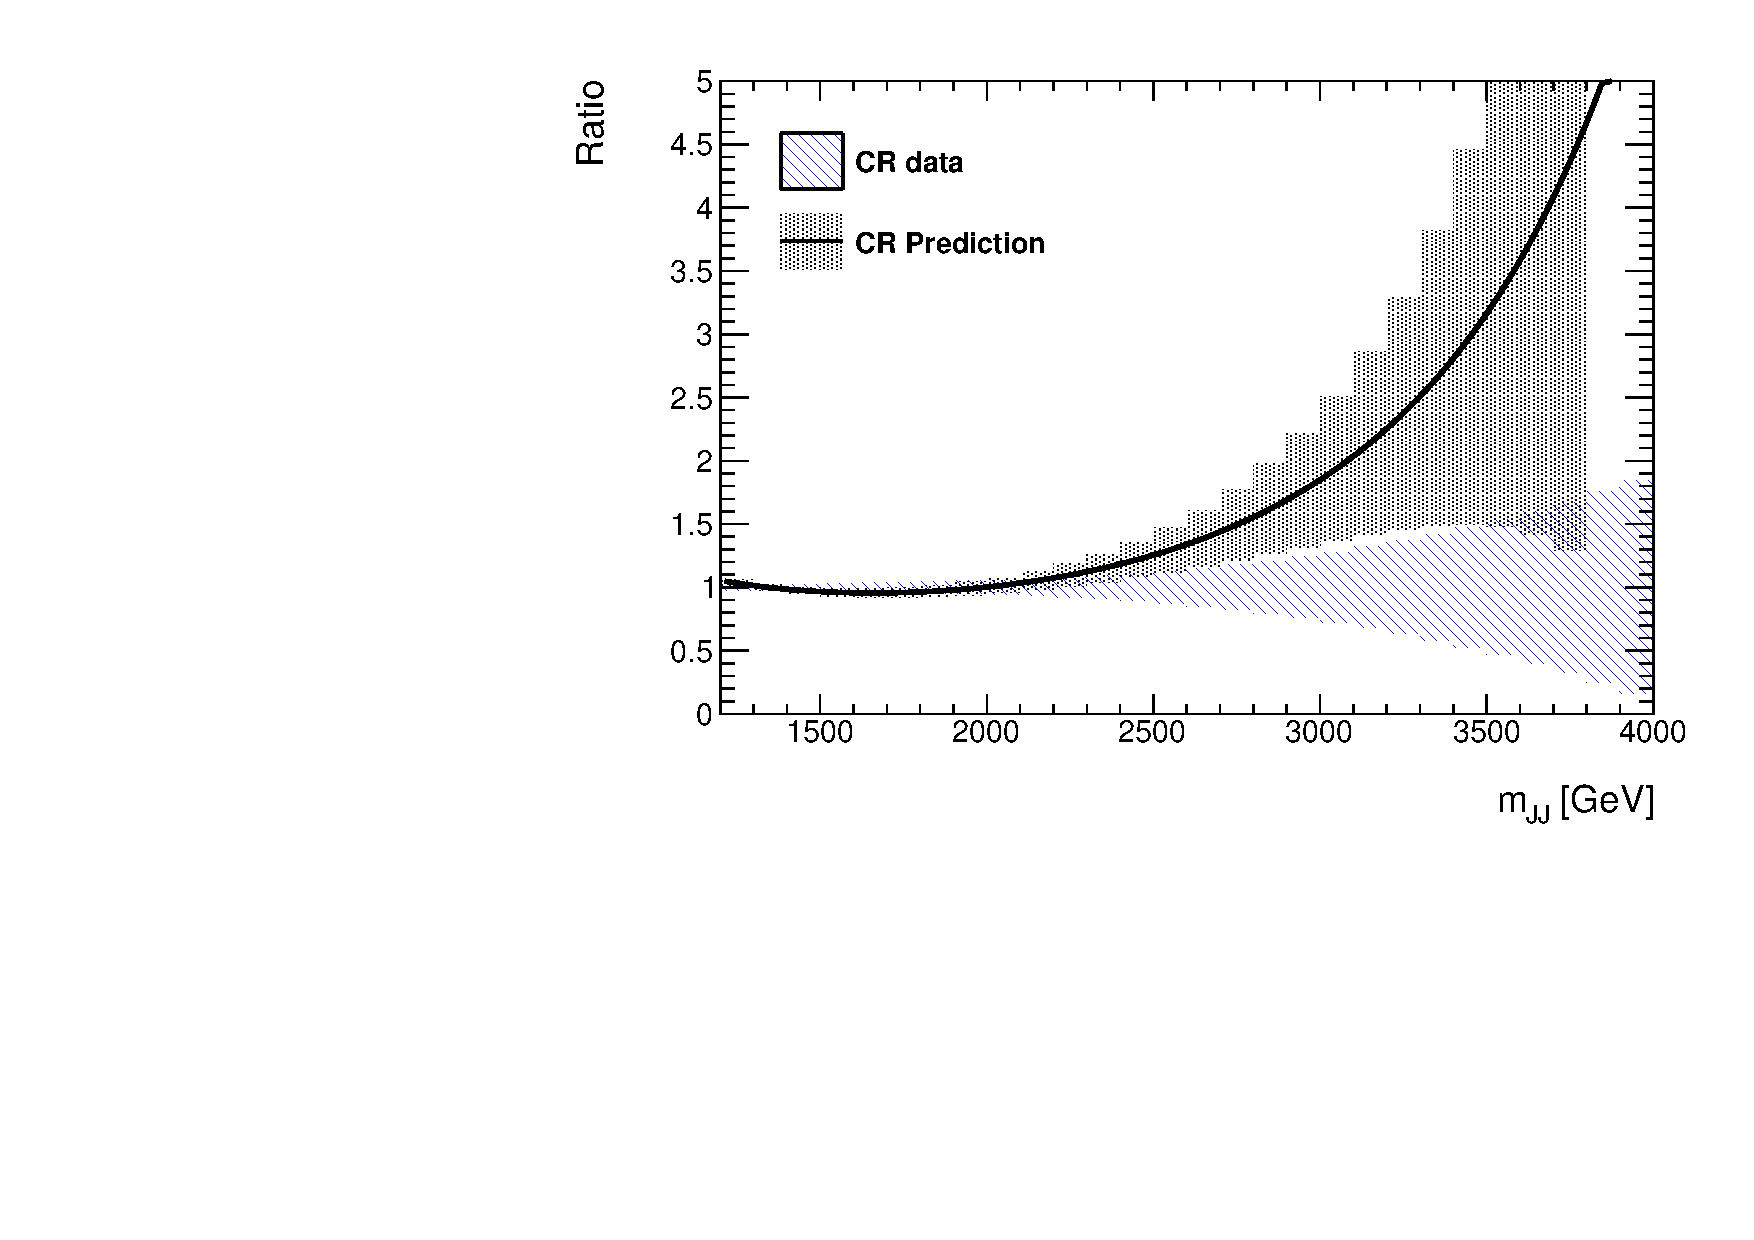
\includegraphics[width=0.31\textwidth,angle=-90]{figures/boosted/Syst_Shape/QCDSysfitSmooth_ratio_22.pdf} \\
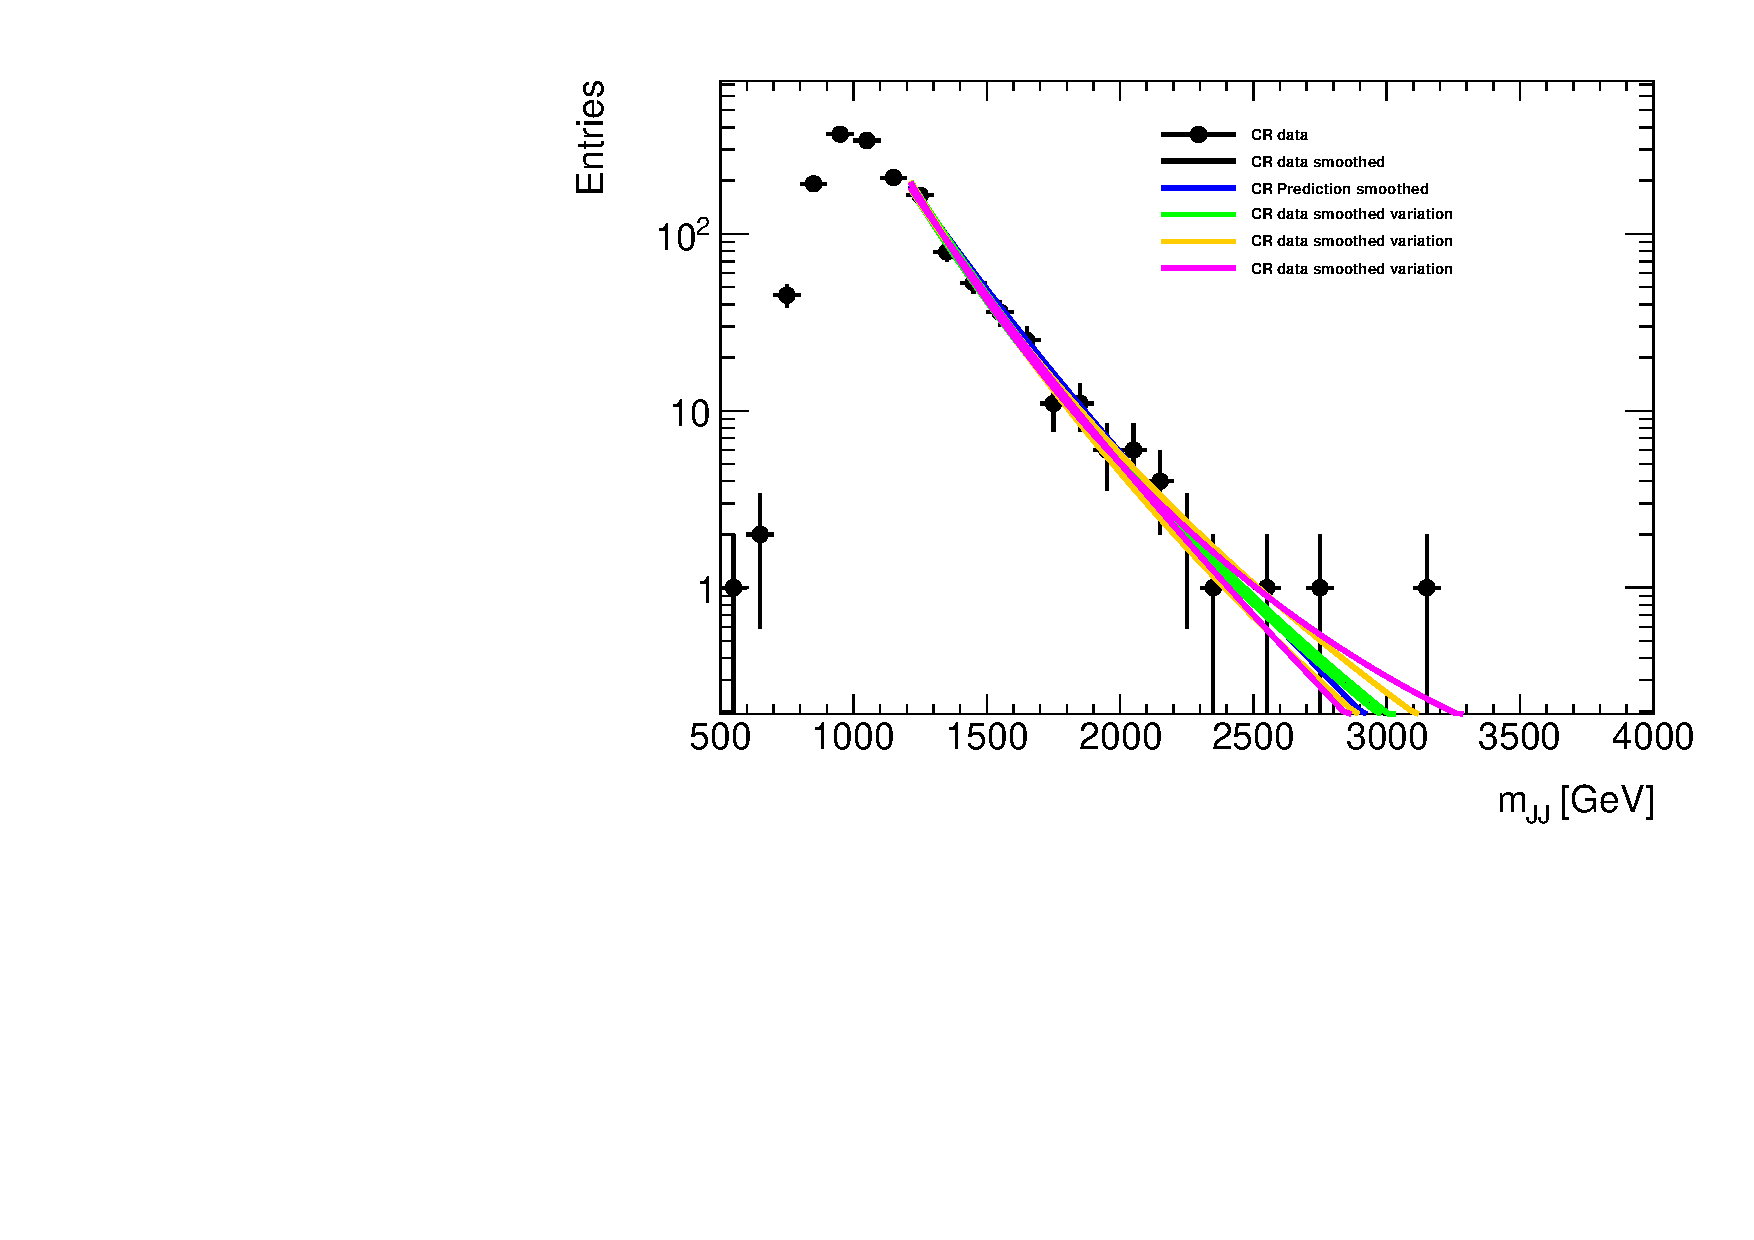
\includegraphics[width=0.31\textwidth,angle=-90]{figures/boosted/Syst_Shape/QCDSysfitSmooth_33.pdf}
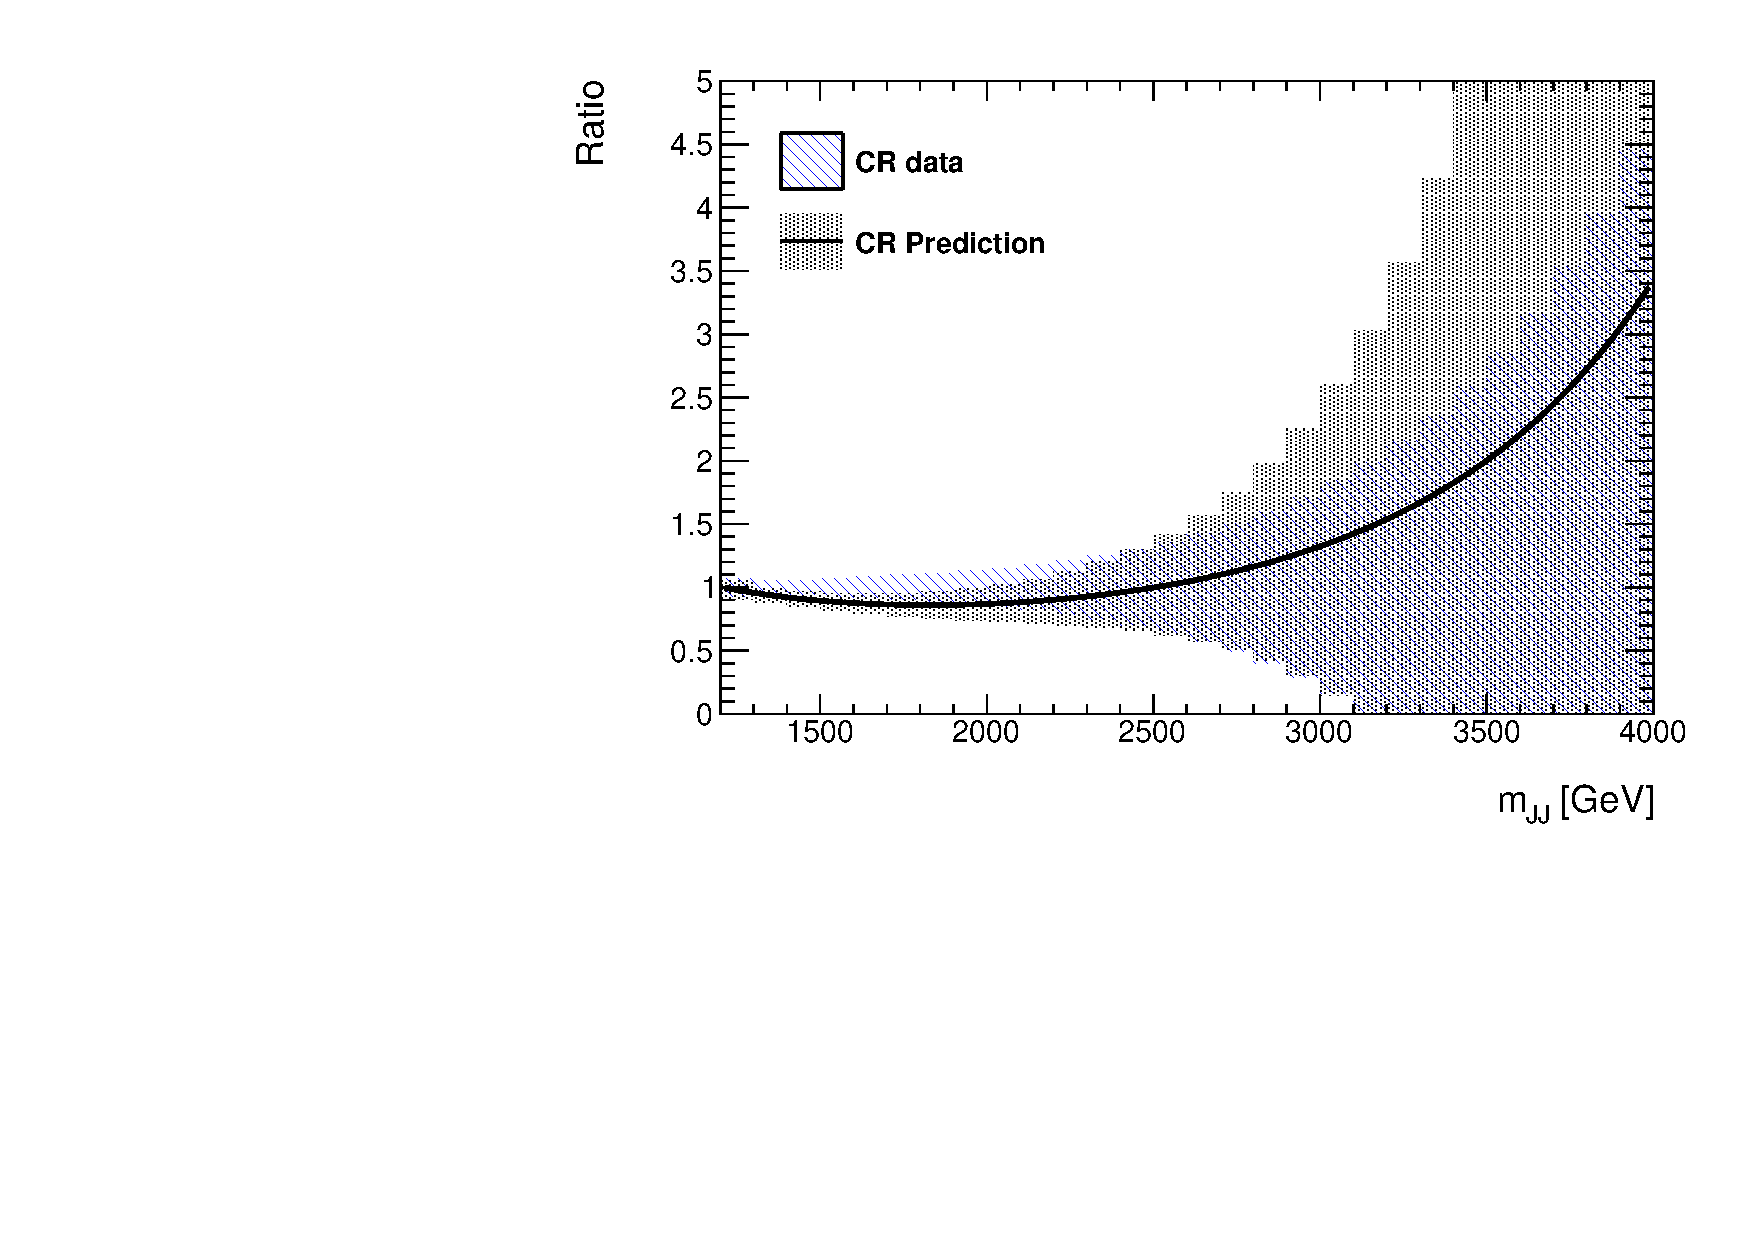
\includegraphics[width=0.31\textwidth,angle=-90]{figures/boosted/Syst_Shape/QCDSysfitSmooth_ratio_33.pdf} \\
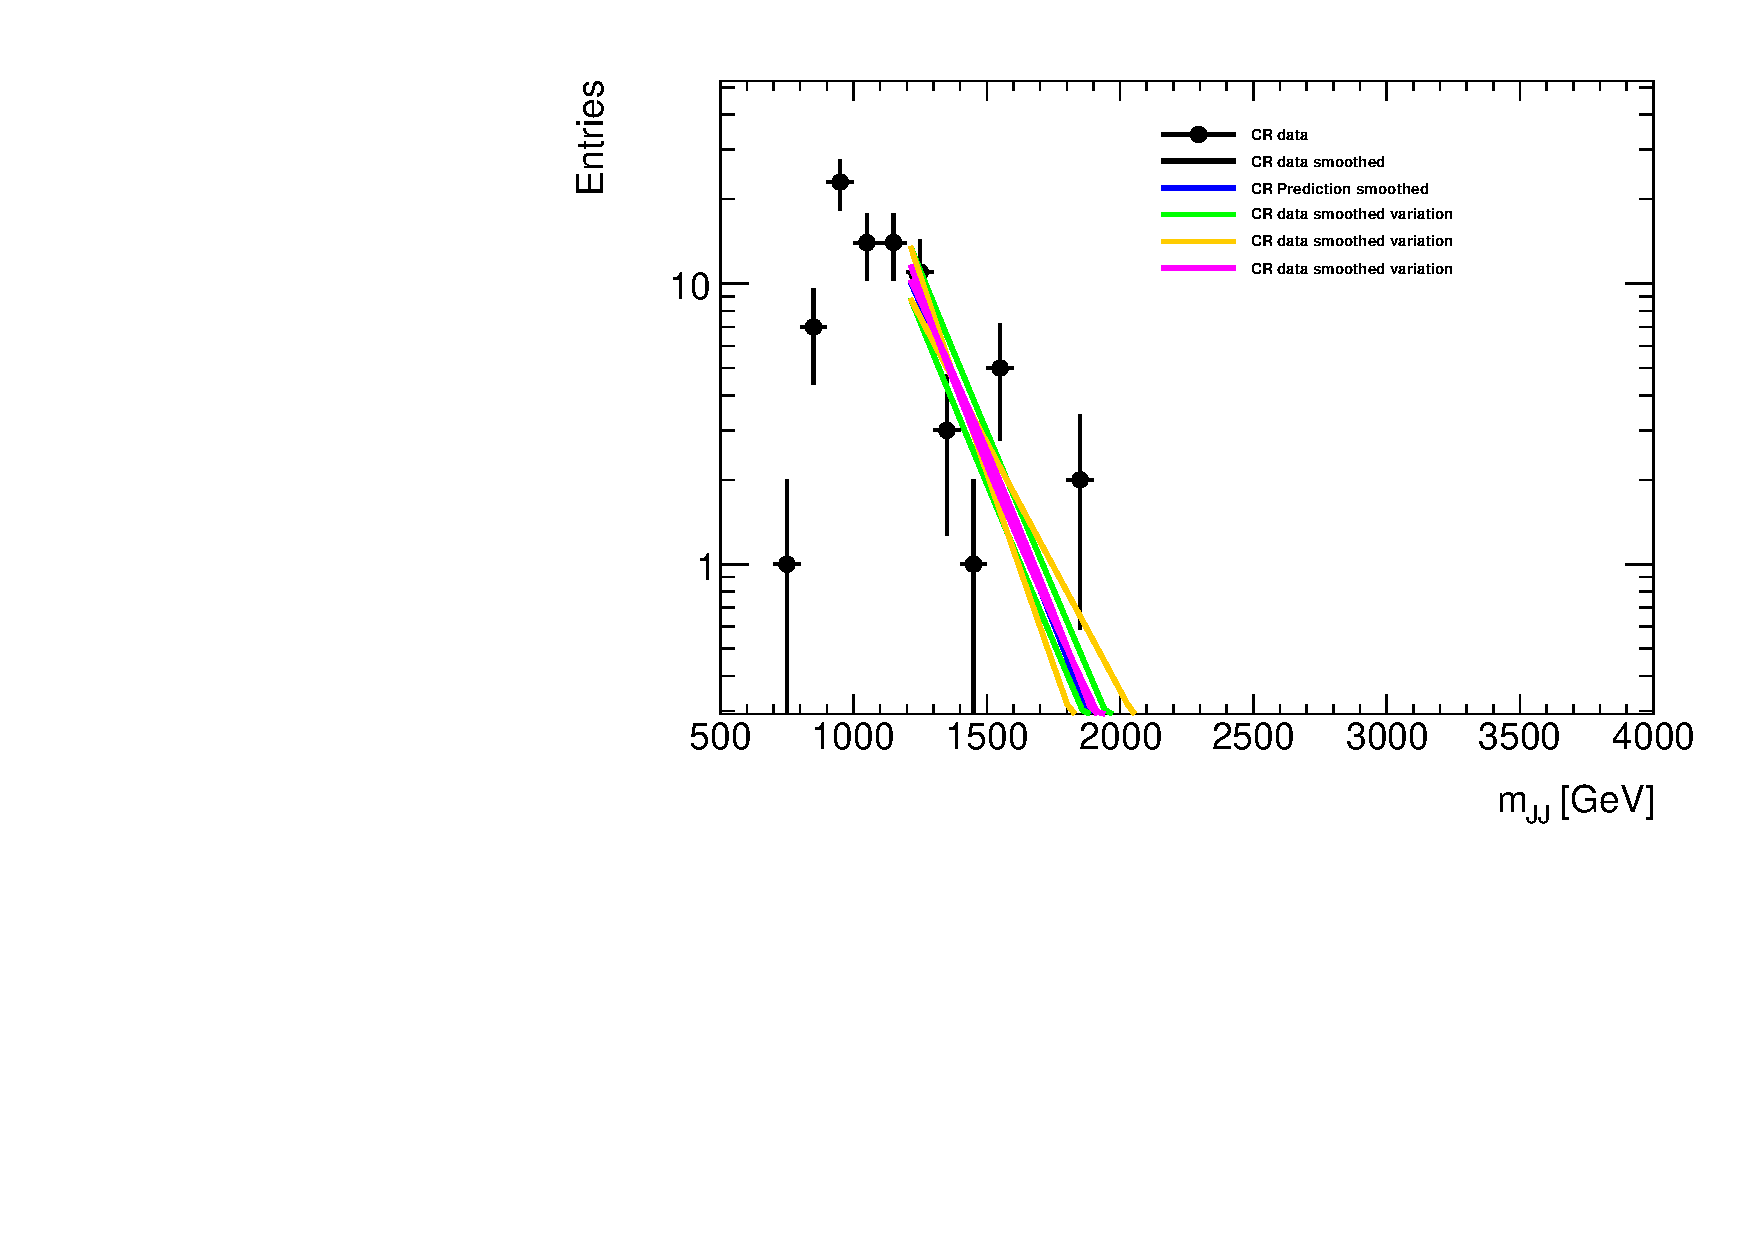
\includegraphics[width=0.31\textwidth,angle=-90]{figures/boosted/Syst_Shape/QCDSysfitSmooth_44.pdf}
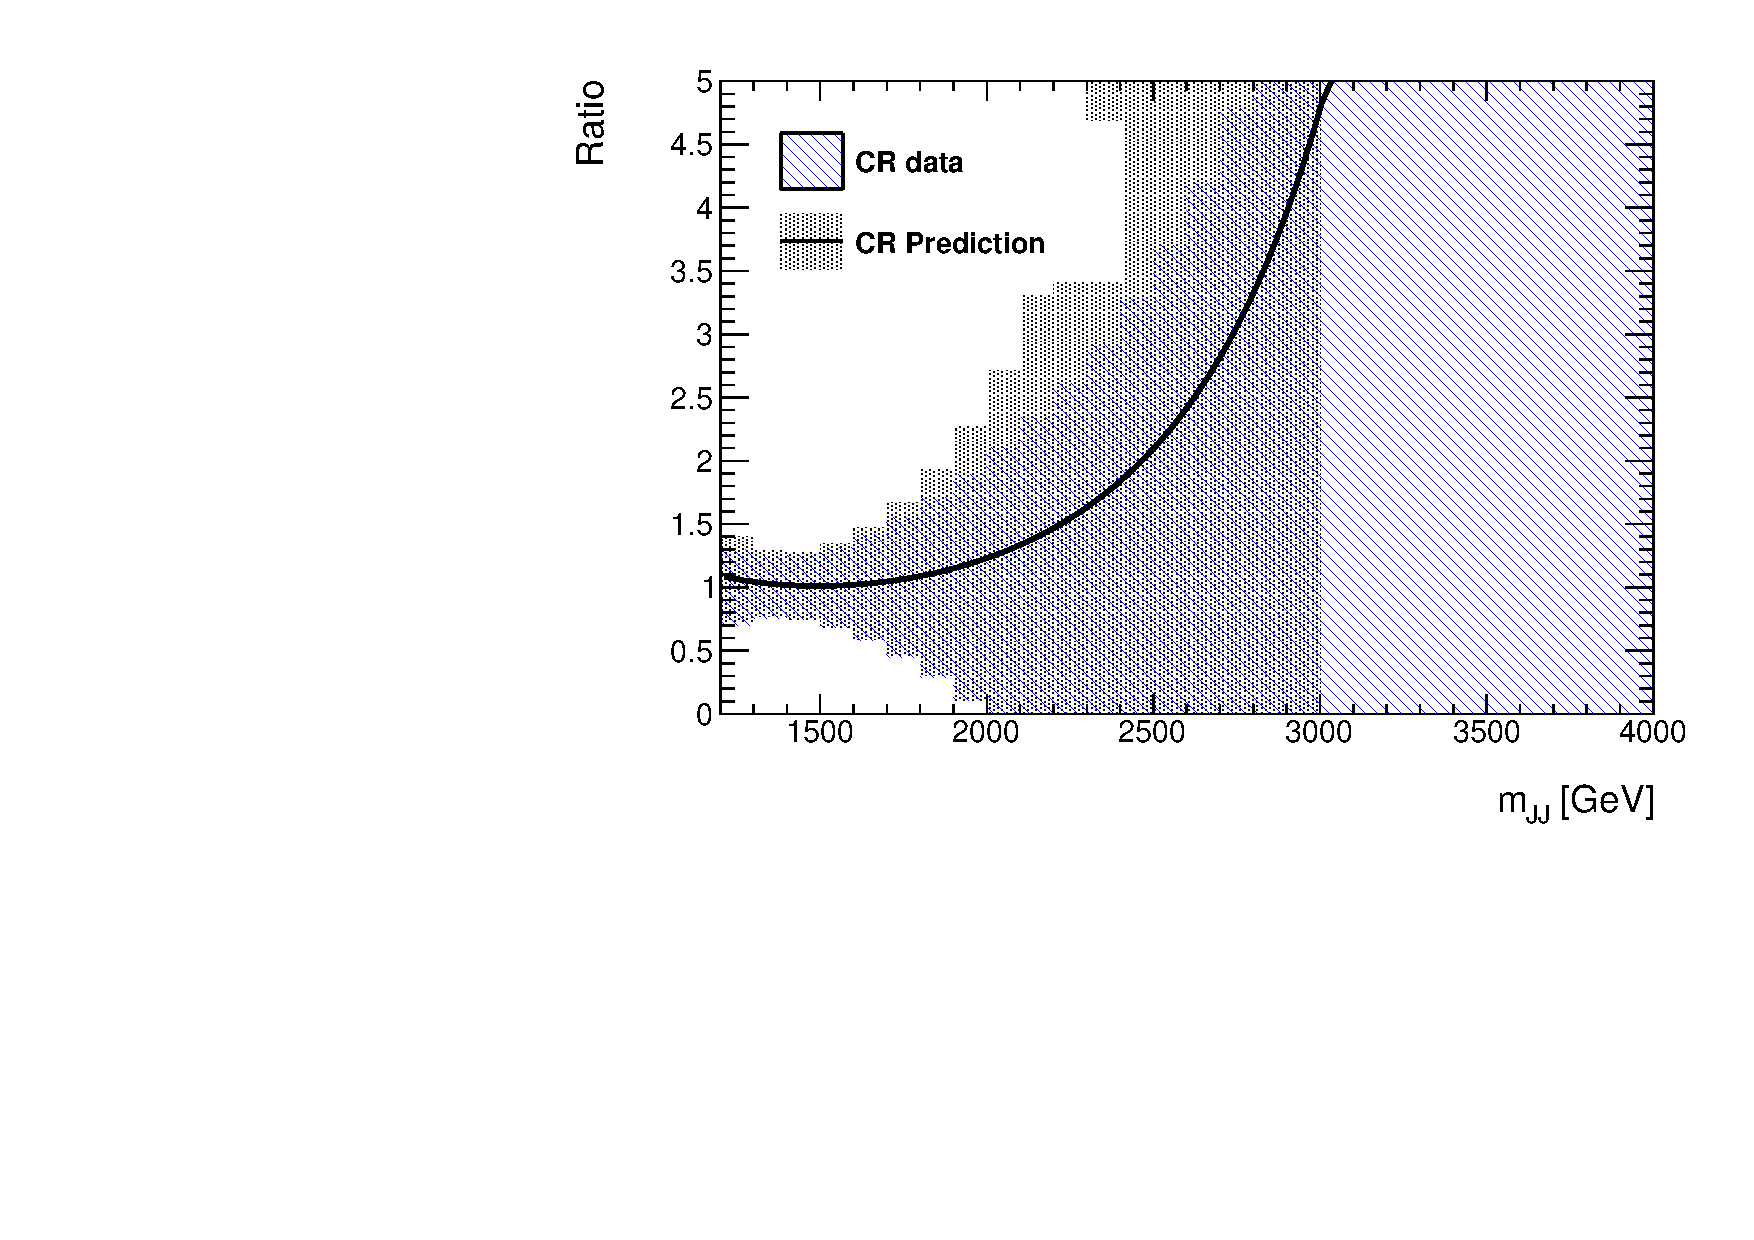
\includegraphics[width=0.31\textwidth,angle=-90]{figures/boosted/Syst_Shape/QCDSysfitSmooth_ratio_44.pdf} \\
\caption{Dijet mass distribution in the CR along with the prediction (left) and the ratio of the prediction to the CR distribution (right)  for the $2bs$ (top) $3b$ (middle) and $4b$ (bottom) samples.  Ratios are from the smoothed distributions, the data uncertainty band contains the smoothing parameter variations, and the prediction uncertainty band also contains smoothing parameter variations.}
\label{fig:qcd_shape_fit}
\end{center}
\end{figure}

\section{Uncertainty on smoothing function in the signal region}
\label{unc-smooth-qcd-in-sr}

\paragraph{}
A specific function has been used to fit the QCD background prediction in order to smooth the distribution and provide non-zero background estimates up to dijet masses beyond enough statistics.  
While this distribution is observed to fit the predicted signal region \mtwoJ~ well, it does not have a concrete physical motivation, and in principle the high mass tail of the distribution could be larger than predicted.
Two checks are performed, changing the boundaries where the fit is performed, and changing the fit function.
The checks shows the smoothing function range and form variations are almost always smaller than the statistical uncertainties of the distributions.
This gives this systematic uncertainty strong correlations with the shape uncertainties discussed in the previous section.
As a result, this systematic uncertainty is excluded.
Nevertheless, the tests are discussed below.

\paragraph{}
To test the impact of the region in which the fit is performed, the upper bound on the dijet fit region are varied to be $\{2800,\ 3000,\ 3200\}$ \GeV and the lower bound are varied to be $\{1200,\ 1300,\ 1400\}$ \GeV.  
The ratio of the fits for each upper bound, to that of the nominal ($1200$-$3000$ \GeV) are shown in Figure~\ref{fig:qcd_fit_range_sys_ratio-scaled}, along with a hash band showing the statistical uncertainty of the nominal fit.
This is estimated separately for $2bs$, $3b$, and $4b$ samples.

\paragraph{}
Fits in which the fit $\chi^2$ probability was less than $0.001\%$, or in which the fit integrals between $1500$-$2000$ \GeV, $2000$-$2500$ \GeV, or $>2500$ \GeV were not in agreement with the original distribution within a factor of $2$ or $0.5$, are not used to estimate the uncertainty. This ensure that poor fits are not used to estimate the uncertainty.

\begin{figure}[htbp!]
\begin{center}
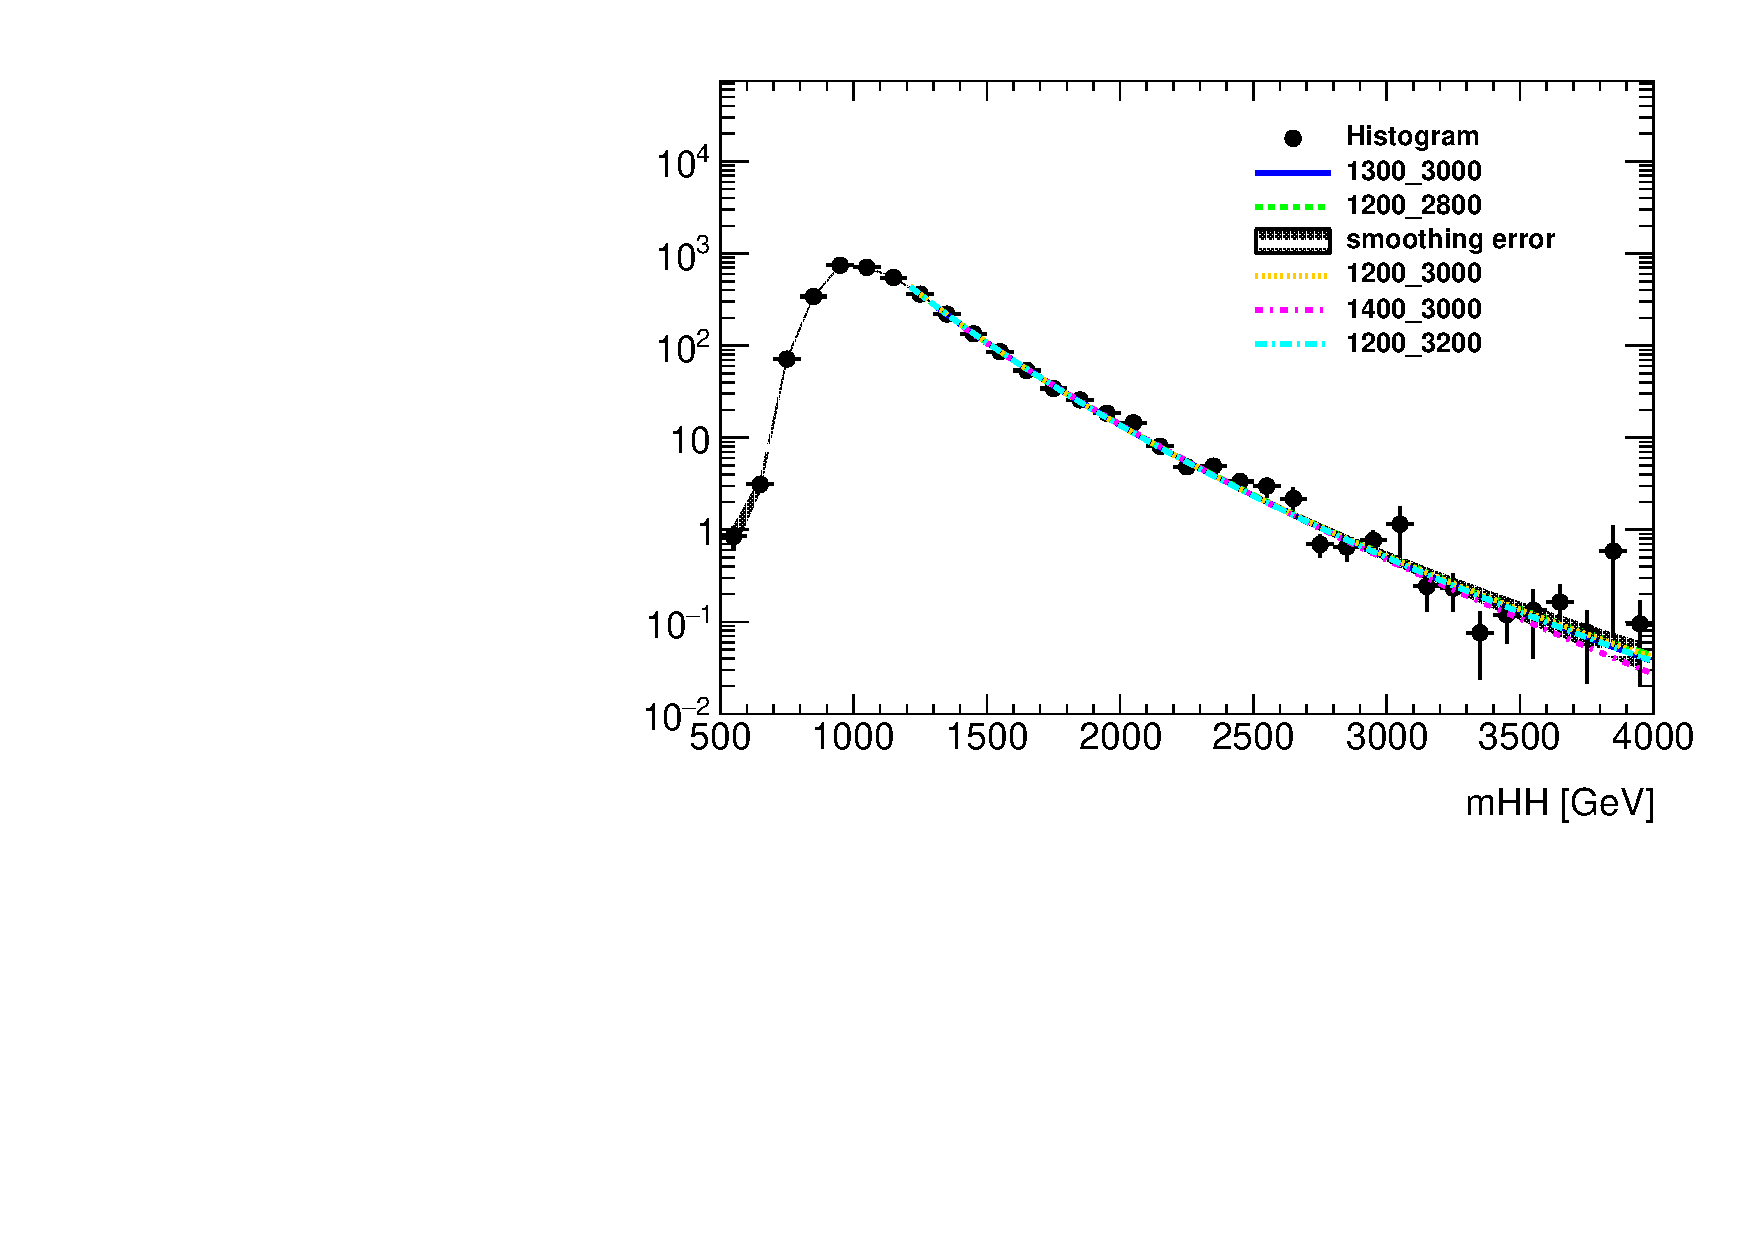
\includegraphics[width=0.31\textwidth,angle=-90]{figures/boosted/Syst_Smooth/smoothFuncRangeCompare_22_comp.pdf}
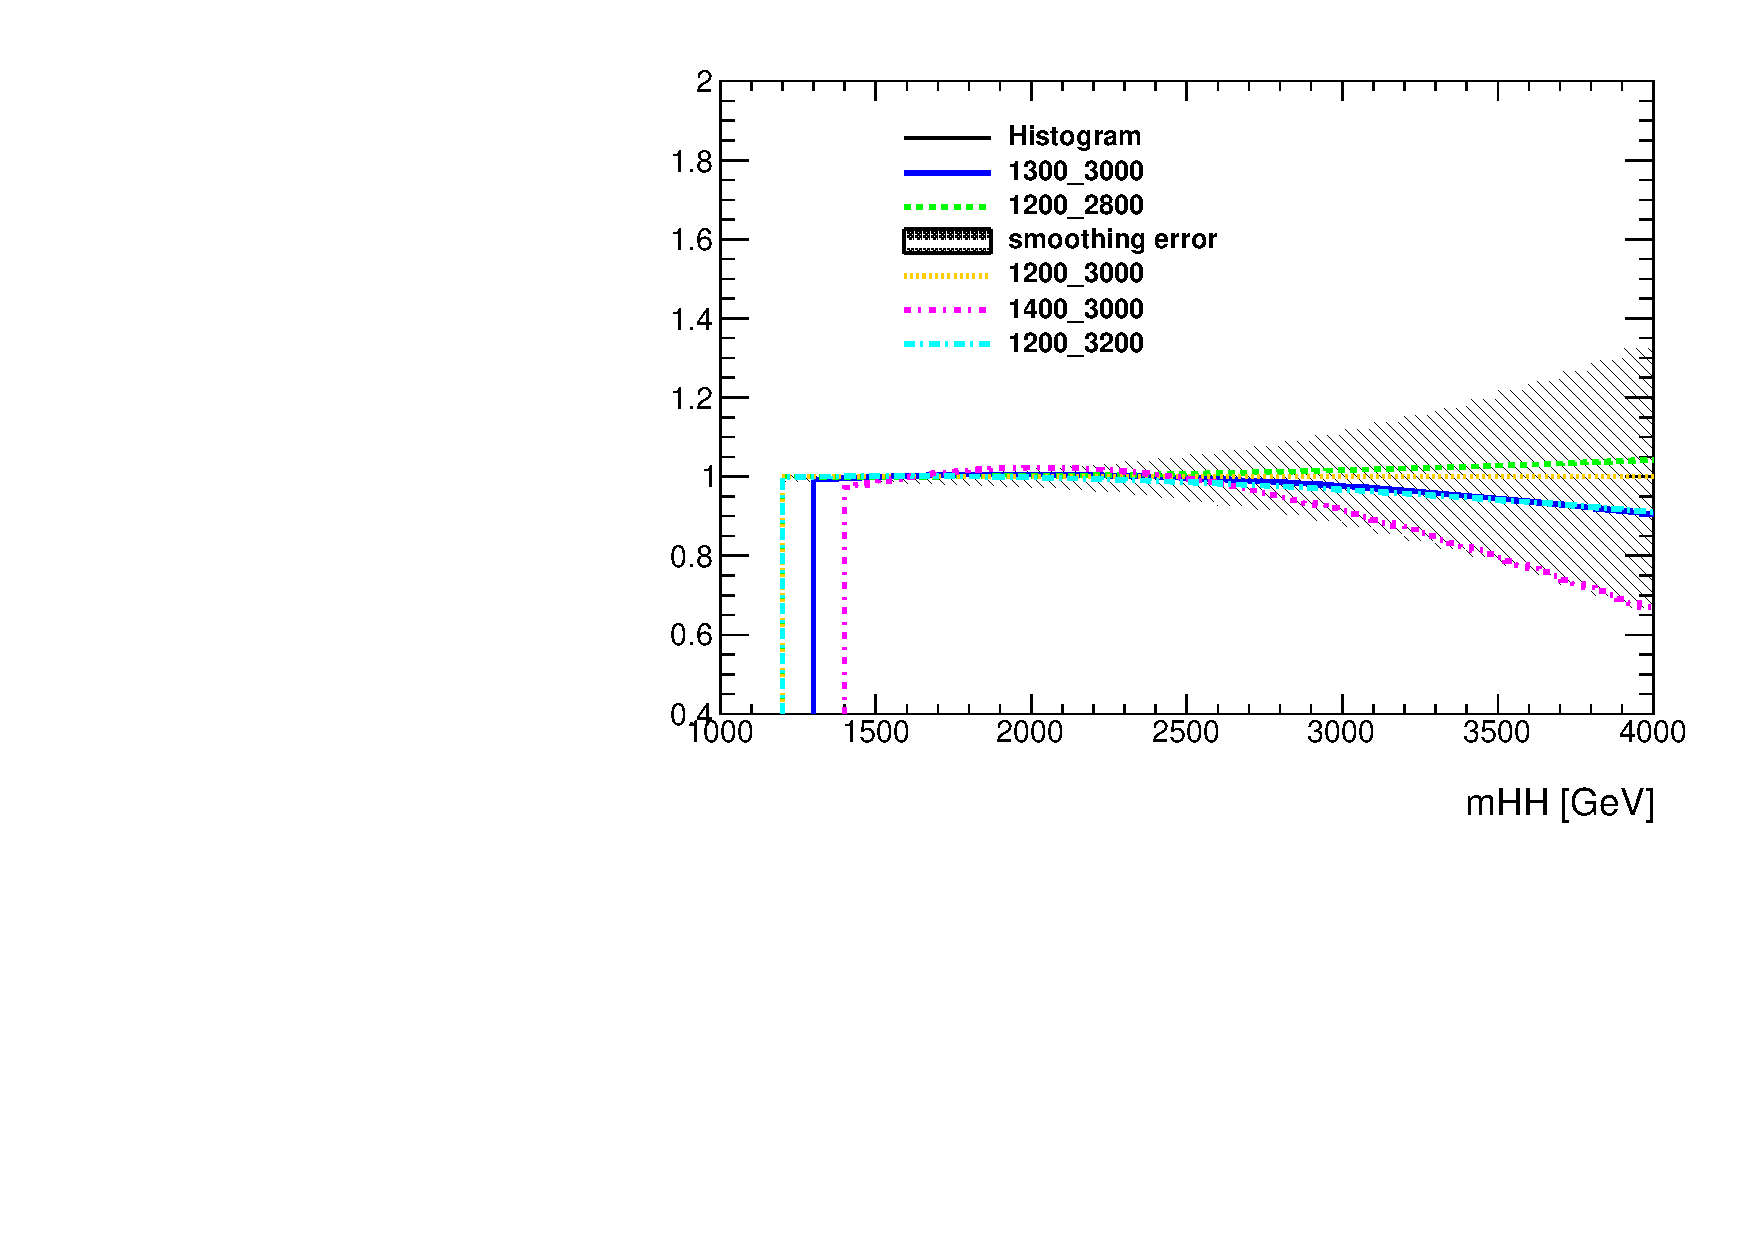
\includegraphics[width=0.31\textwidth,angle=-90]{figures/boosted/Syst_Smooth/smoothFuncRangeCompare_22_comp_ratio.pdf} \\
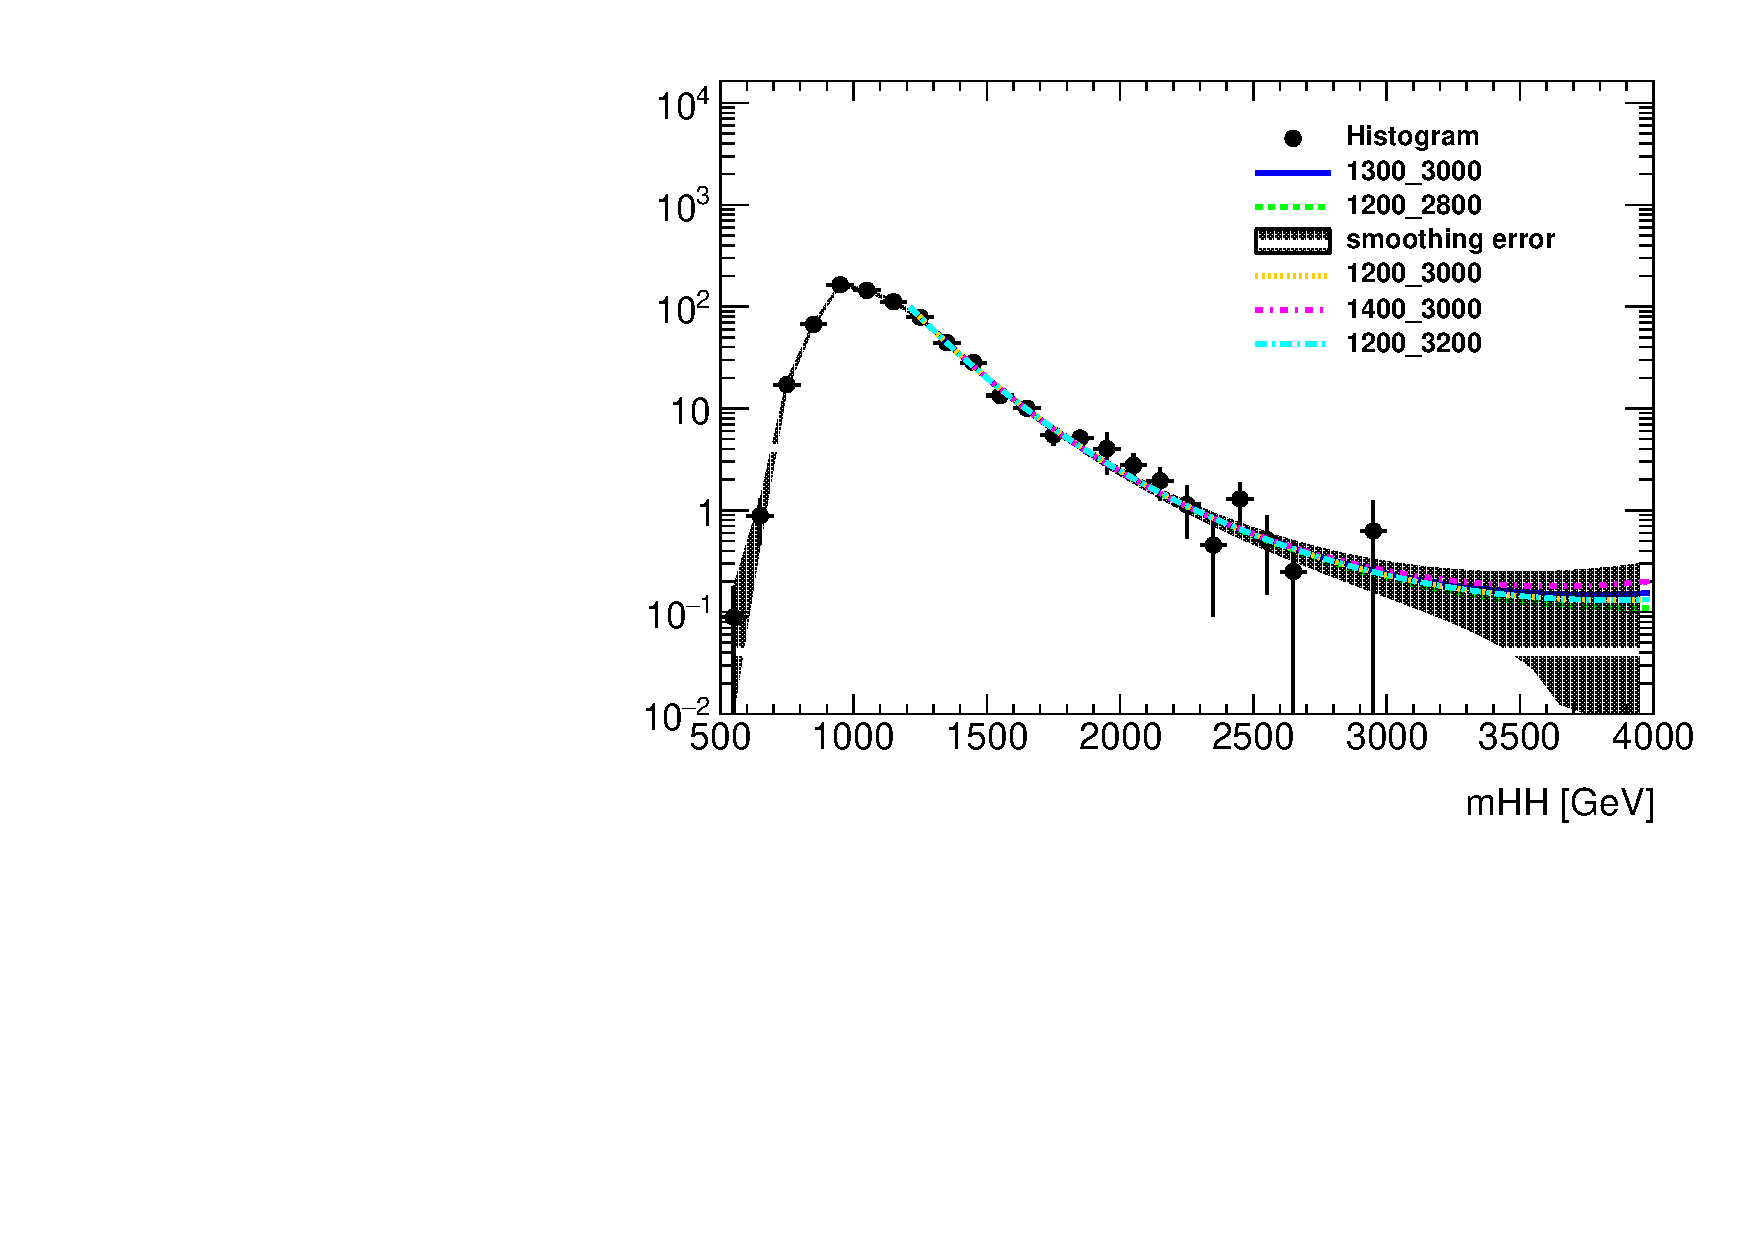
\includegraphics[width=0.31\textwidth,angle=-90]{figures/boosted/Syst_Smooth/smoothFuncRangeCompare_33_comp.pdf}
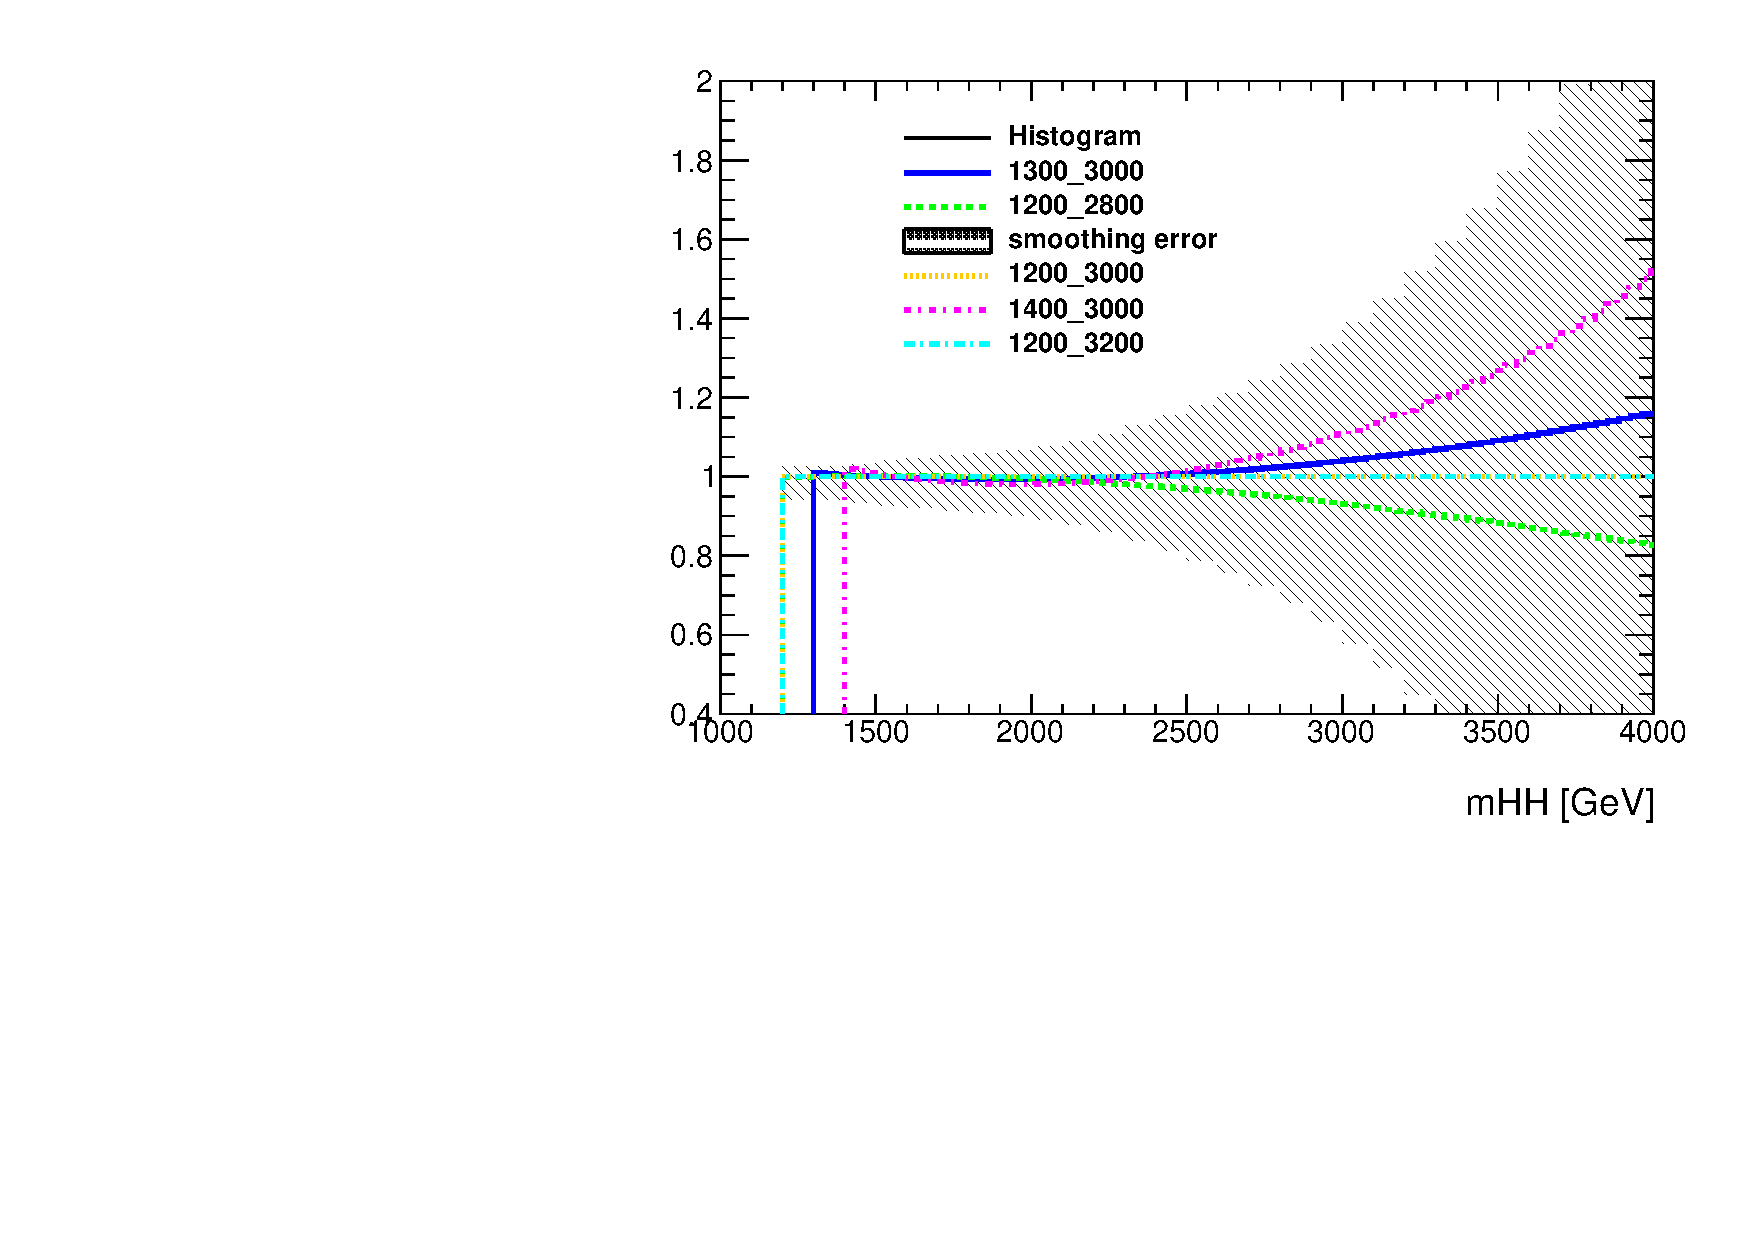
\includegraphics[width=0.31\textwidth,angle=-90]{figures/boosted/Syst_Smooth/smoothFuncRangeCompare_33_comp_ratio.pdf} \\
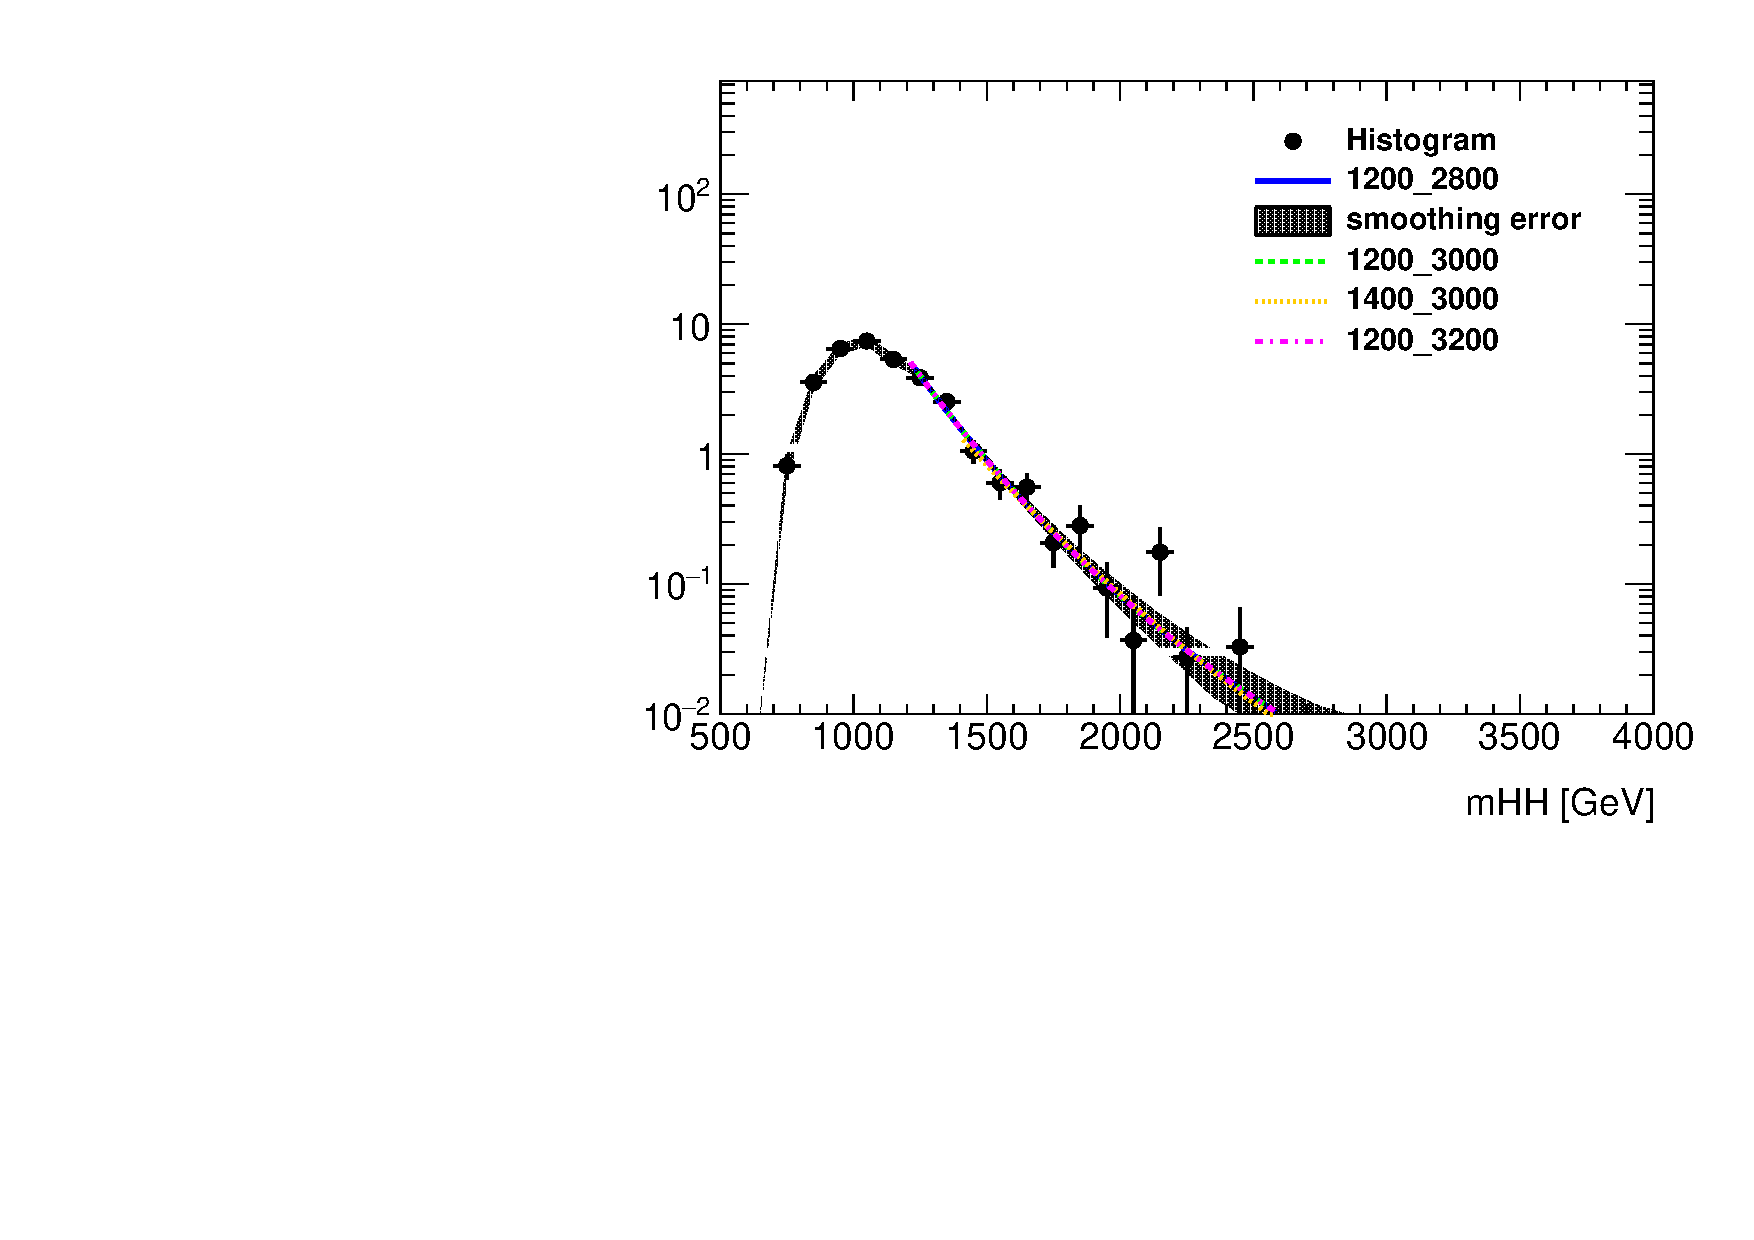
\includegraphics[width=0.31\textwidth,angle=-90]{figures/boosted/Syst_Smooth/smoothFuncRangeCompare_44_comp.pdf}
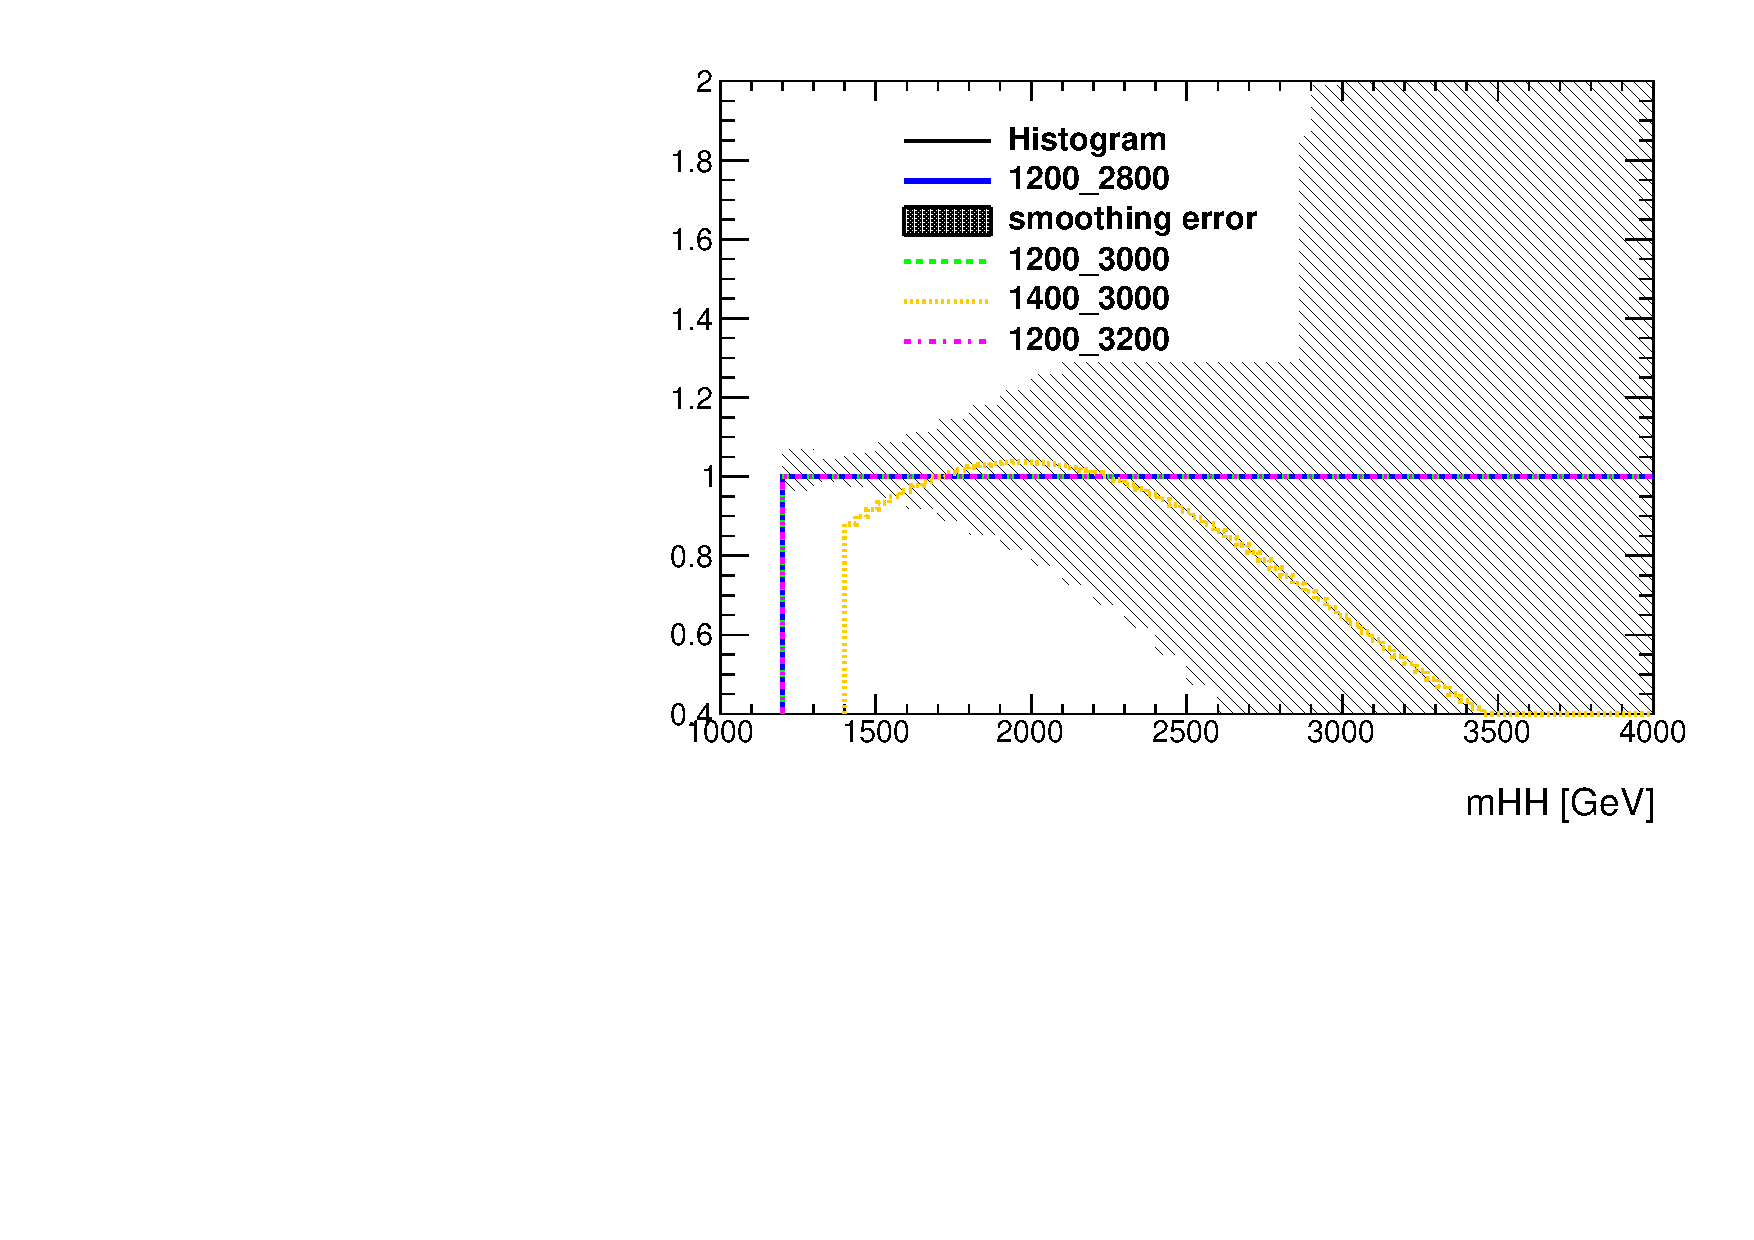
\includegraphics[width=0.31\textwidth,angle=-90]{figures/boosted/Syst_Smooth/smoothFuncRangeCompare_44_comp_ratio.pdf} \\
\caption{Dijet mass distribution SR prediction fit with several fit ranges (left) and the ratio of nominal to fits with different fit ranges (right)  for the $2bs$ (top) $3b$ (middle) and $4b$ (bottom) samples. }
\label{fig:qcd_fit_range_sys_ratio-scaled}
\end{center}
\end{figure}

\paragraph{}
The signal region QCD prediction is also fitted with a variety of other distributions which can show both power law behavior in the bulk of the distribution. 
The set of additional functions examined (labeled MJ1-MJ7) can be found in Table~\ref{tab:fit_funcs}, where $x = m_{JJ} / \sqrt{s}$.

\begin{table}[htbp!]
\begin{center} 
\begin{tabular}{  l | c}
Name & Functional Form \\
\hline
MJ1 (Dijet) & $f_{1}(x) = p_0 (1-x)^{p_1} x^{p_2}$ \\
MJ2 & $f_{2}(x) = p_0 (1-x)^{p_1} e^{p_2\ x^2}$ \\
MJ3 & $f_{3}(x) = p_0 (1-x)^{p_1} x^{p_2\ x}$ \\
MJ4 & $f_{4}(x) = p_0 (1-x)^{p_1} x^{p_2\ ln\ x}$ \\
MJ5 & $f_{5}(x) = p_0 (1-x)^{p_1} (1+x)^{p_2\ x}$ \\
MJ6 & $f_{6}(x) = p_0 (1-x)^{p_1} (1+x)^{p_2\ ln\ x}$ \\
MJ7 & $f_{7}(x) = \frac{p_0}{x} (1-x)^{p_1 - p_2\ ln\ x}$ \\
MJ8 & $f_{8}(x) = \frac{p_0}{x^2} (1-x)^{p_1 - p_2\ ln\ x}$ \\
\hline
\end{tabular}
\caption{Functions used to fit the QCD dijet mass distributions, where $x = m_{JJ} / \sqrt{s}$.}
\label{tab:fit_funcs}
\end{center}
\end{table}

\paragraph{}
Figure~\ref{fig:qcd_fit_funcs_sys} shows the fits to the QCD prediction in the $4/3/2bs$ signal regions, and the nominal dijet fit, as well as the ratios of the nominal fit to that of the additional functions.
As before, poor fits are not used to estimate the uncertainty..

\begin{figure}[htbp!]
\begin{center}
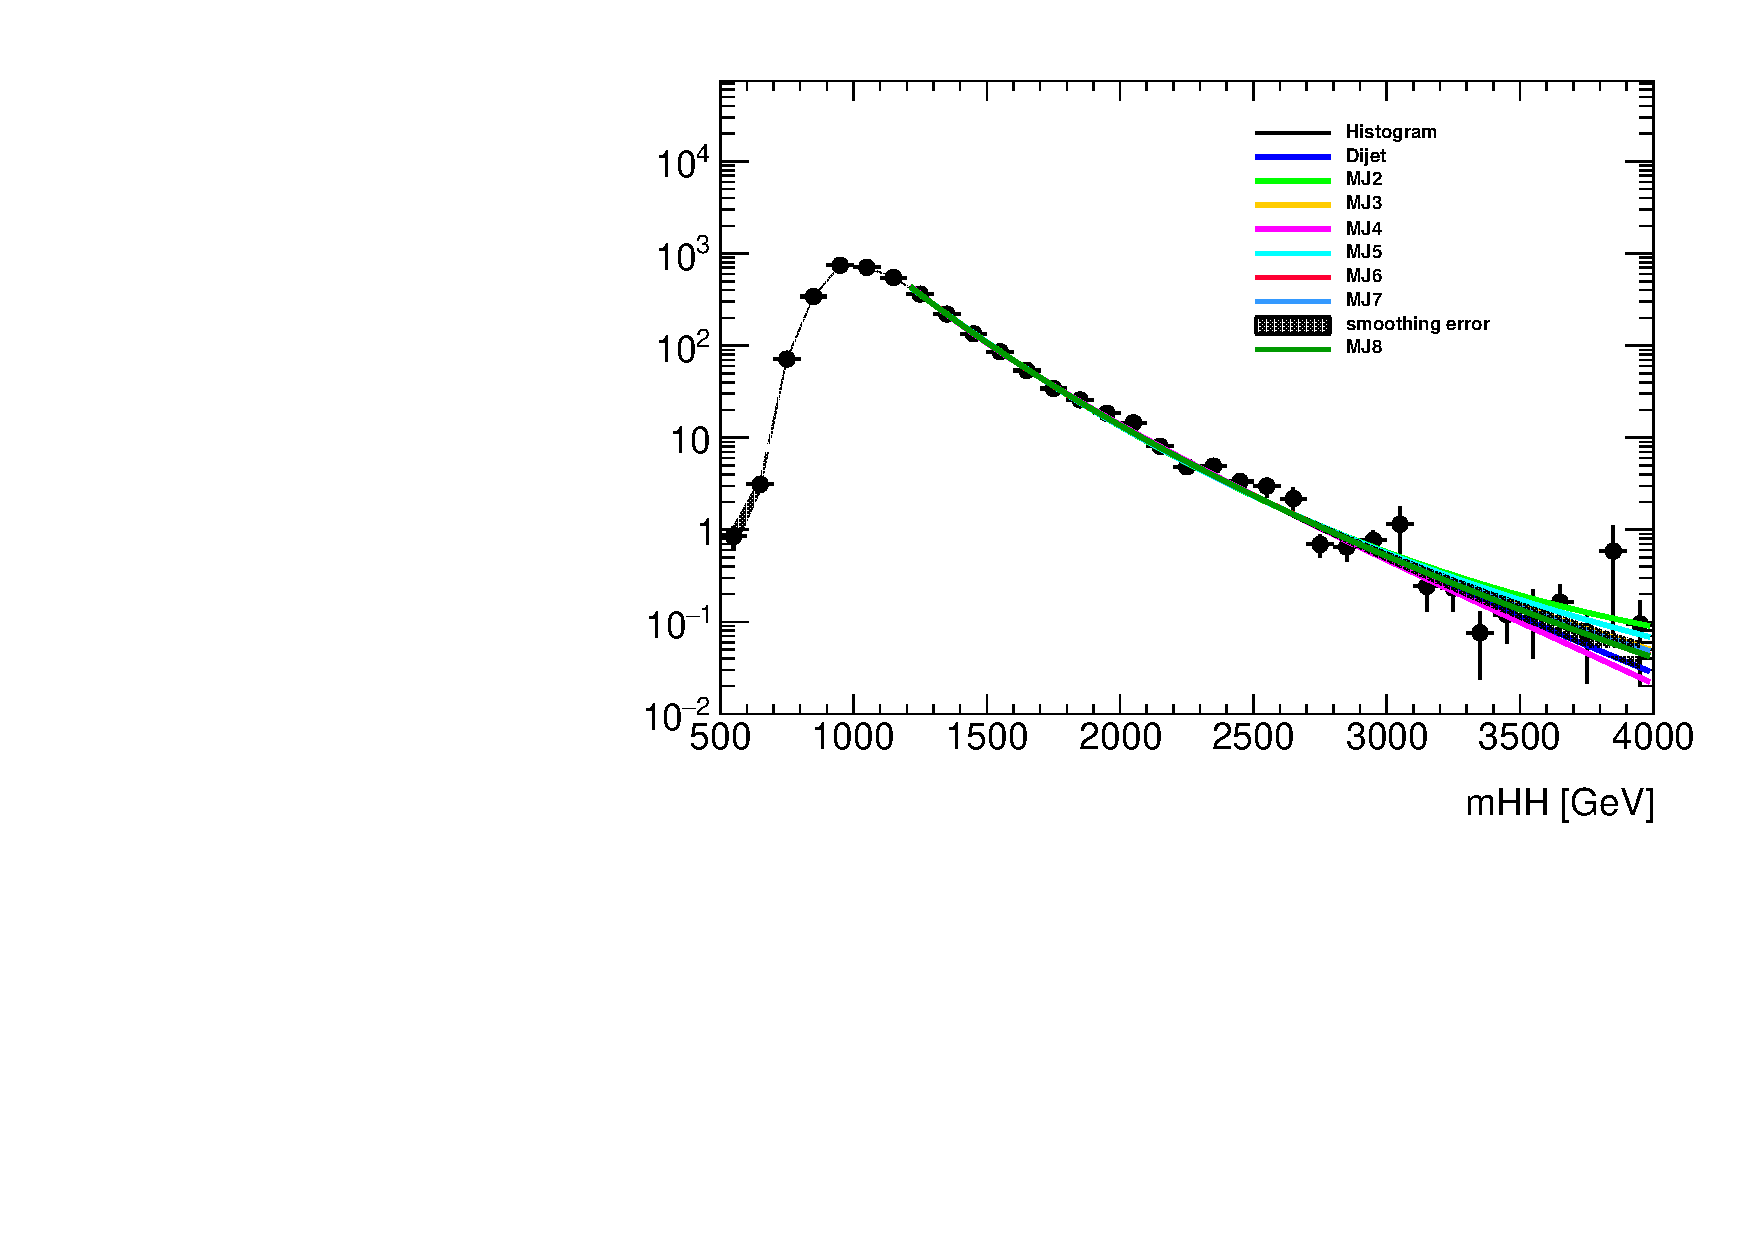
\includegraphics[width=0.31\textwidth,angle=-90]{figures/boosted/Syst_Smooth/smoothFuncCompare_22_comp.pdf}
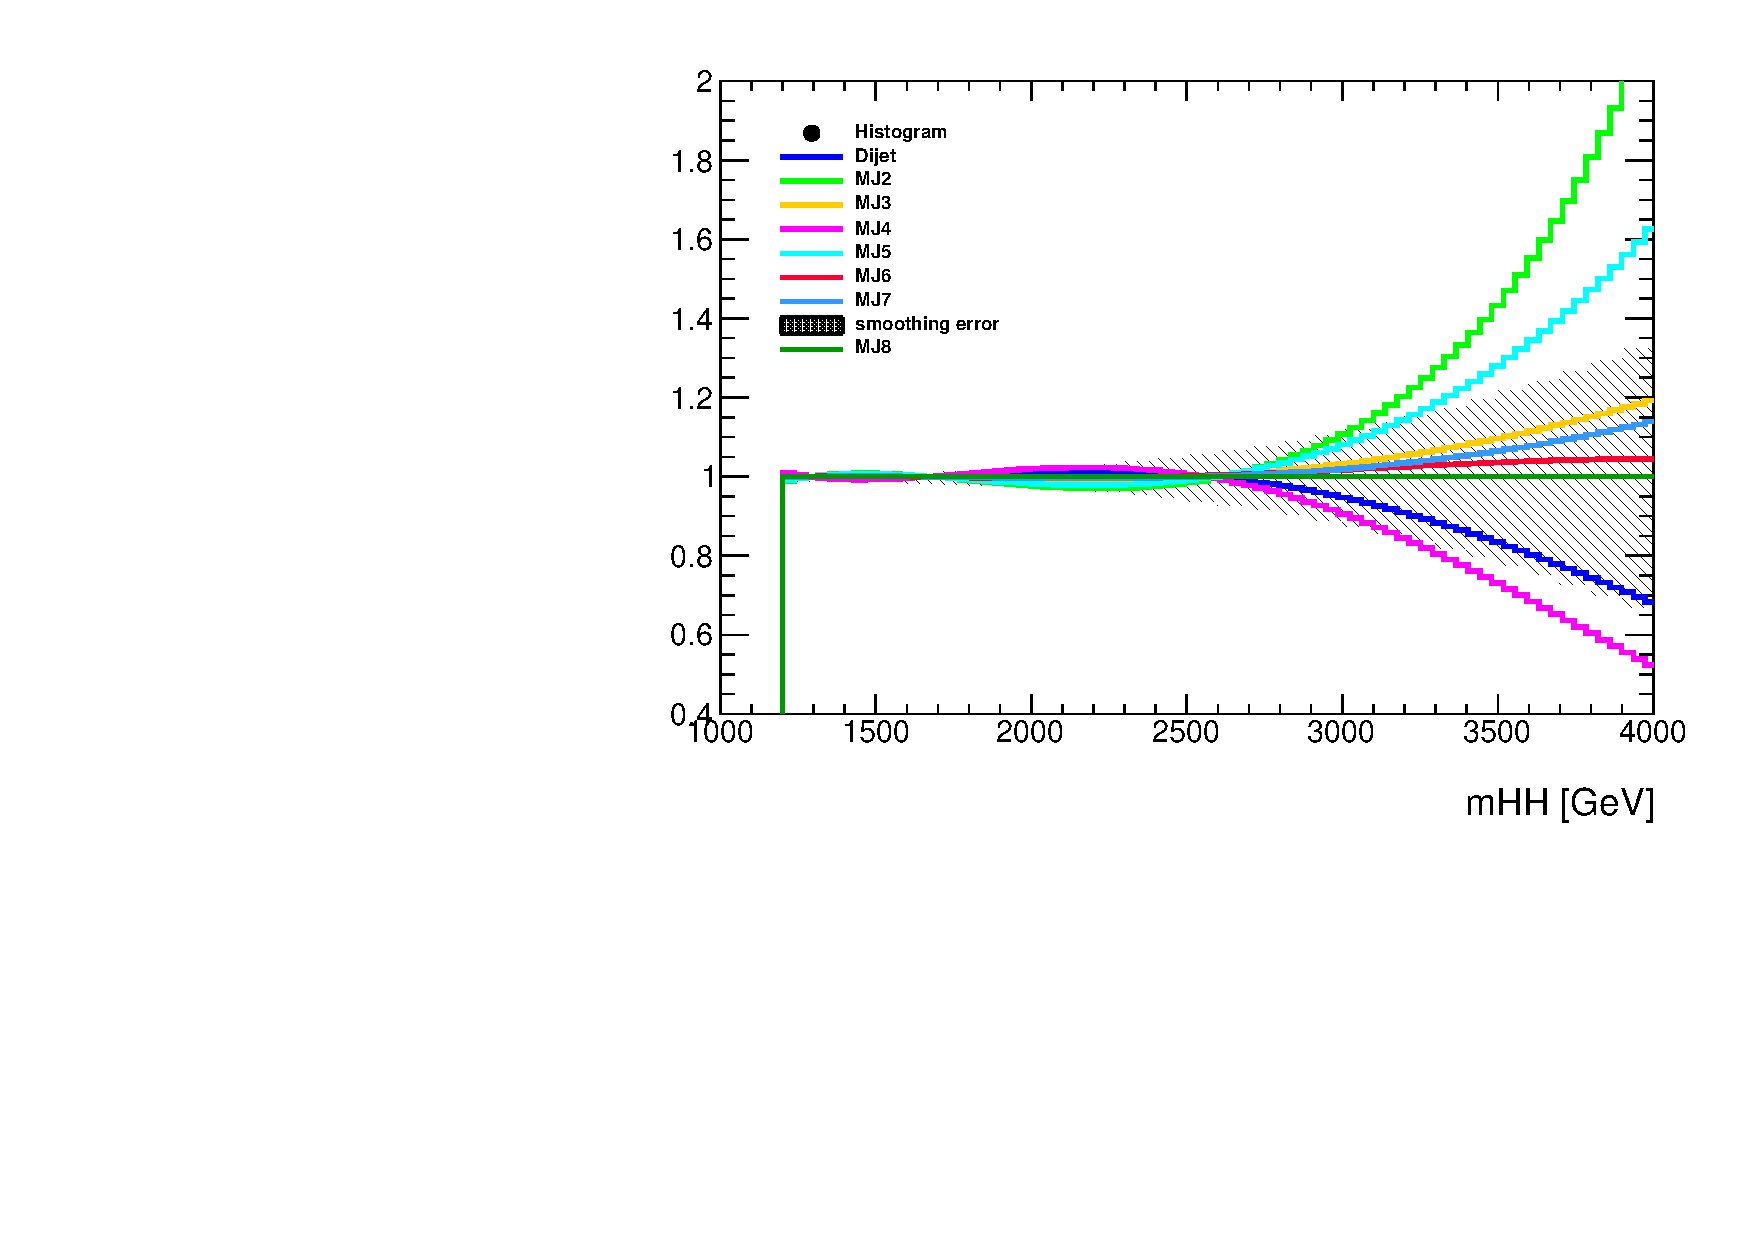
\includegraphics[width=0.31\textwidth,angle=-90]{figures/boosted/Syst_Smooth/smoothFuncCompare_22_comp_ratio.pdf} \\
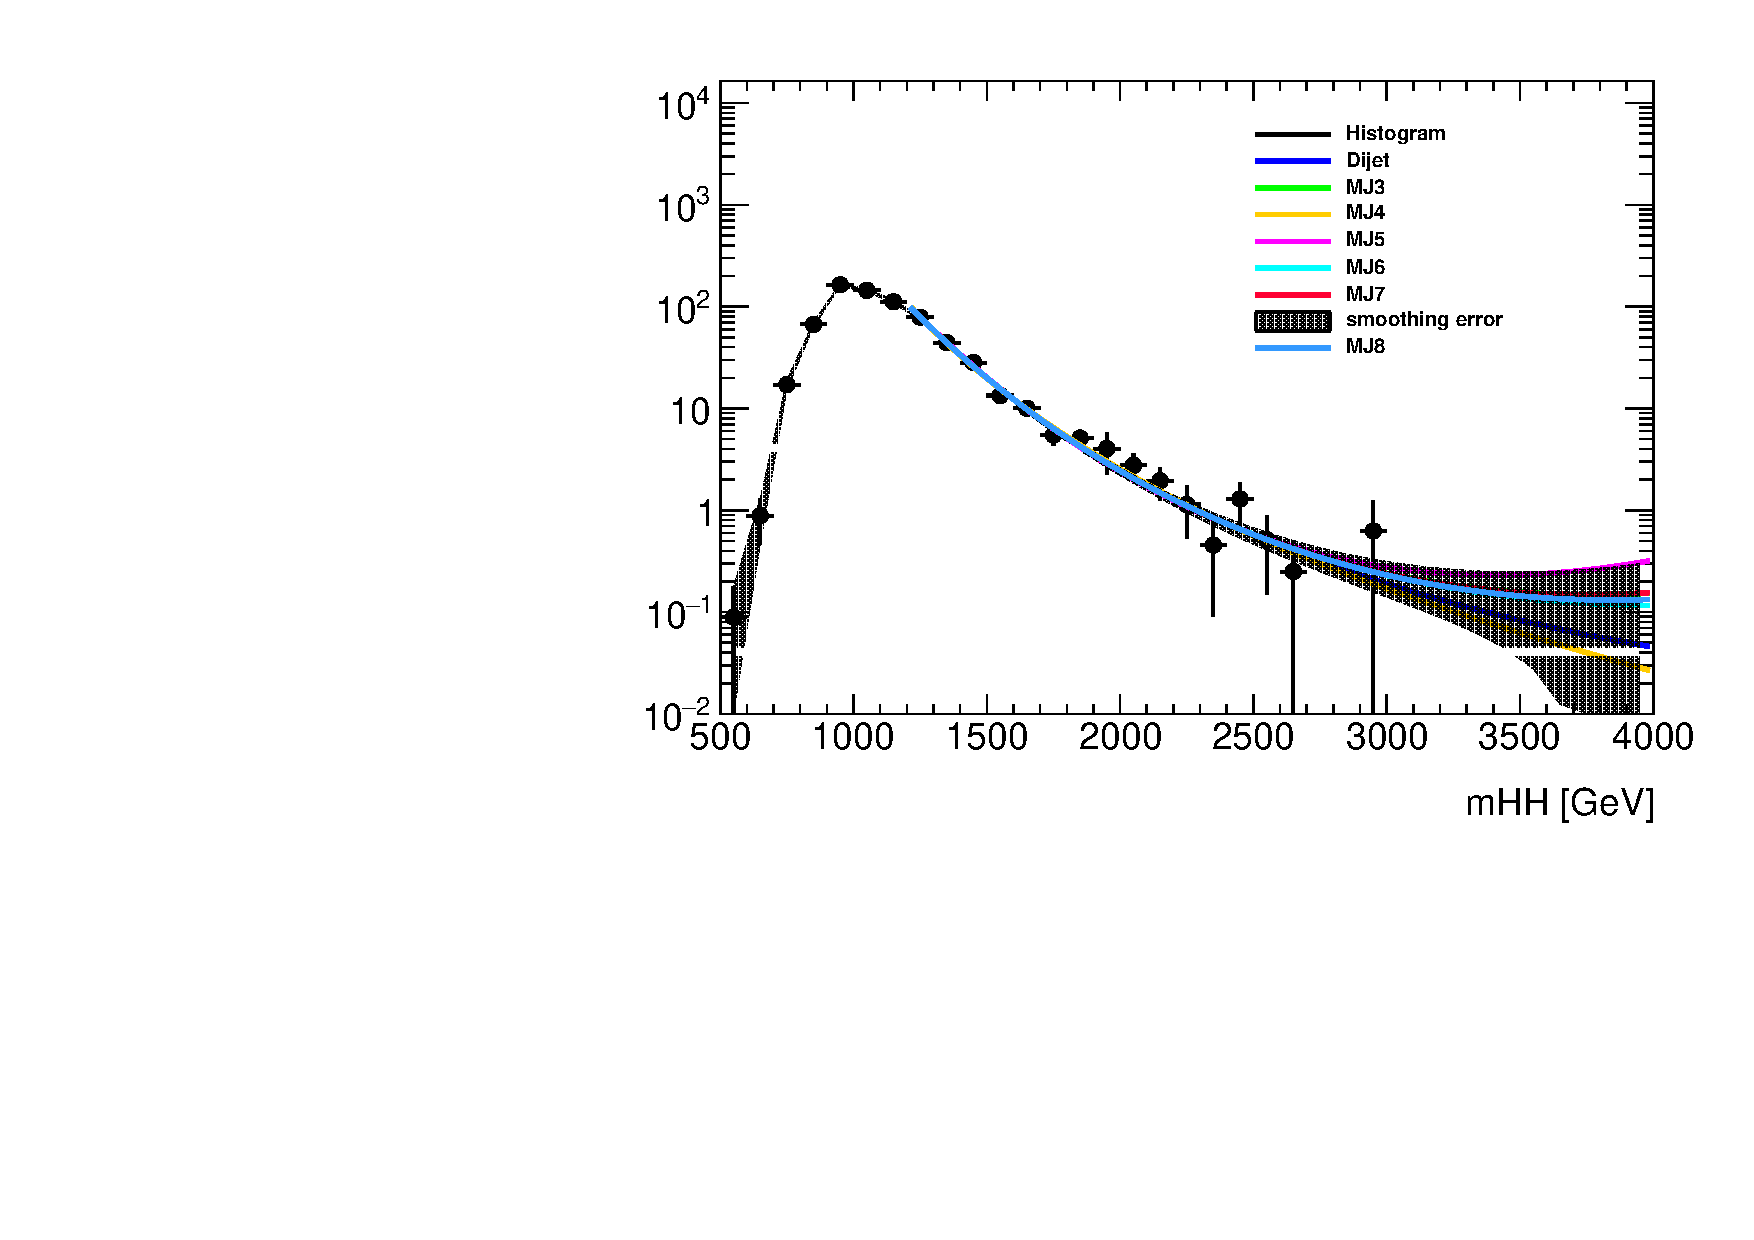
\includegraphics[width=0.31\textwidth,angle=-90]{figures/boosted/Syst_Smooth/smoothFuncCompare_33_comp.pdf}
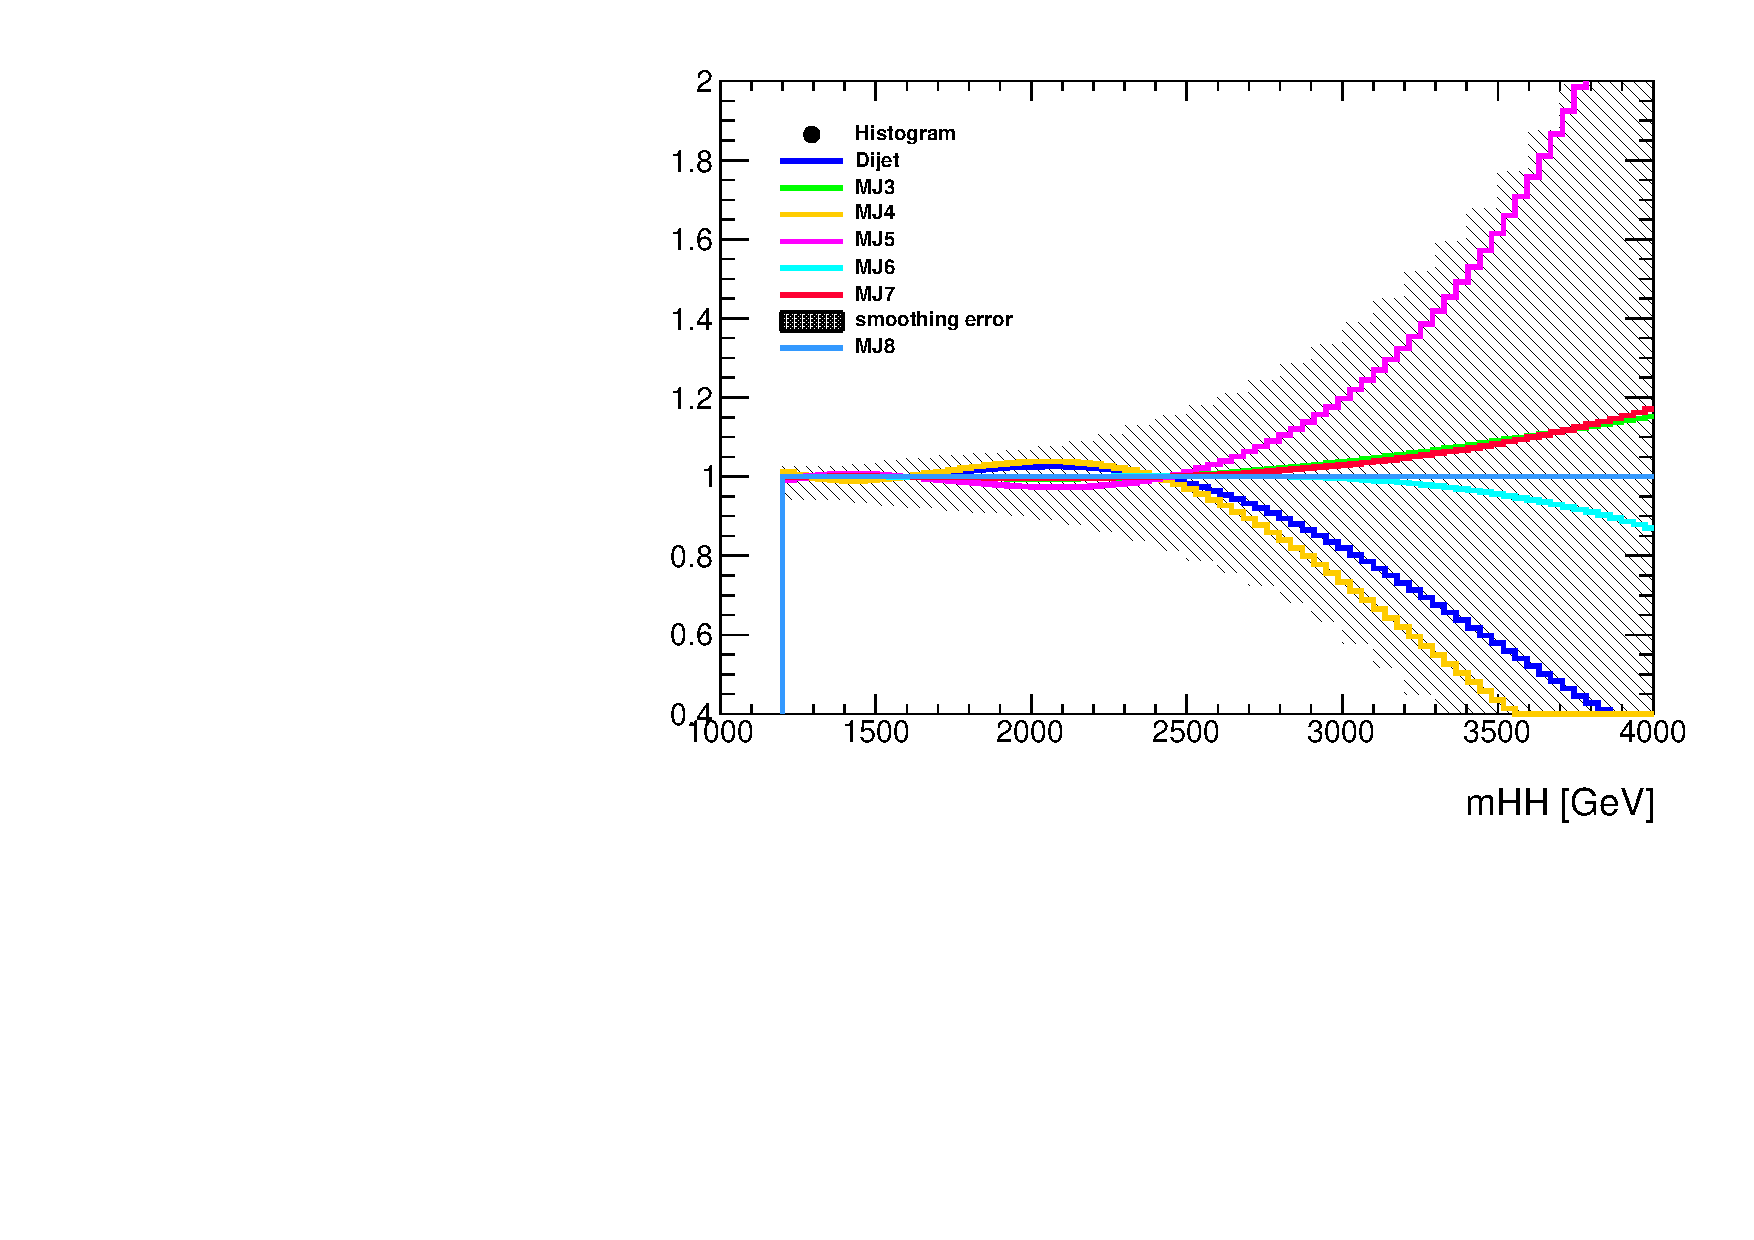
\includegraphics[width=0.31\textwidth,angle=-90]{figures/boosted/Syst_Smooth/smoothFuncCompare_33_comp_ratio.pdf} \\
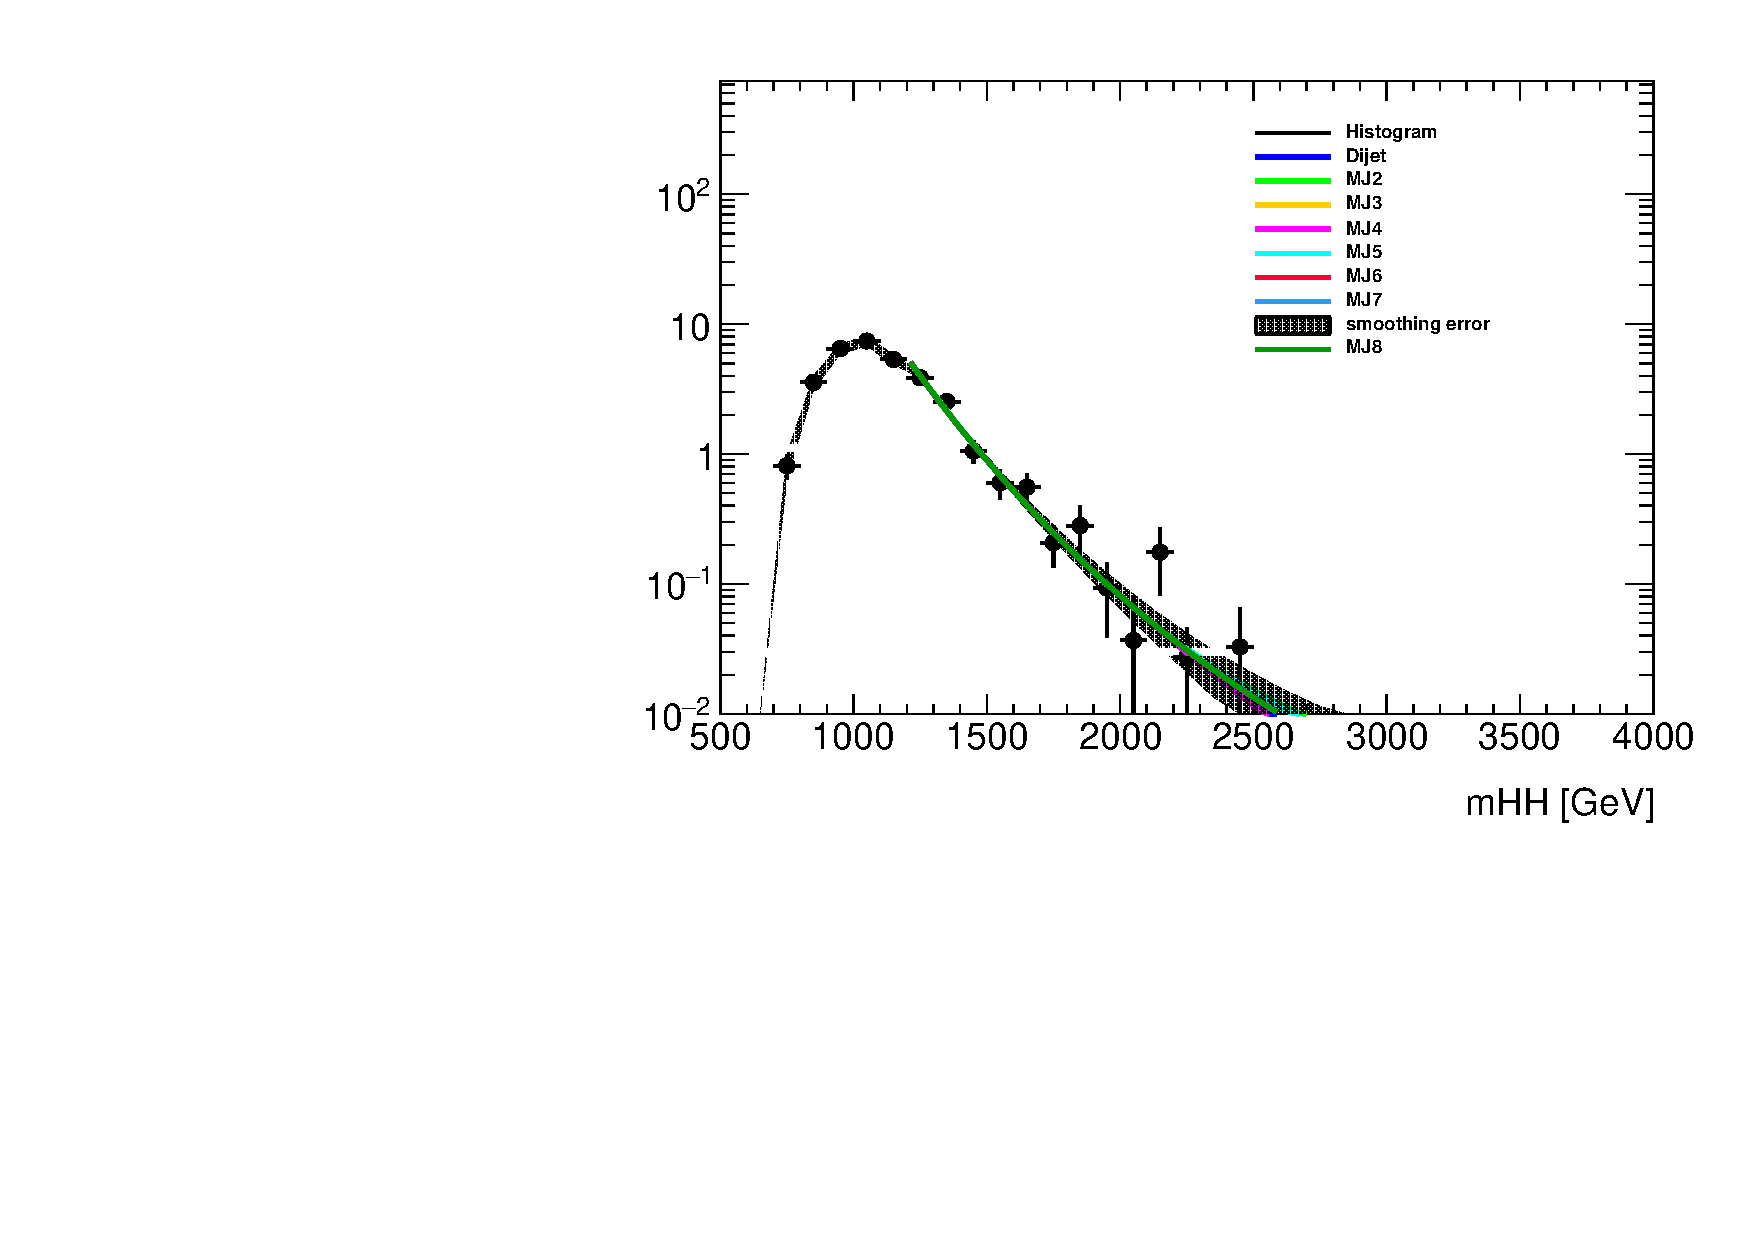
\includegraphics[width=0.31\textwidth,angle=-90]{figures/boosted/Syst_Smooth/smoothFuncCompare_44_comp.pdf}
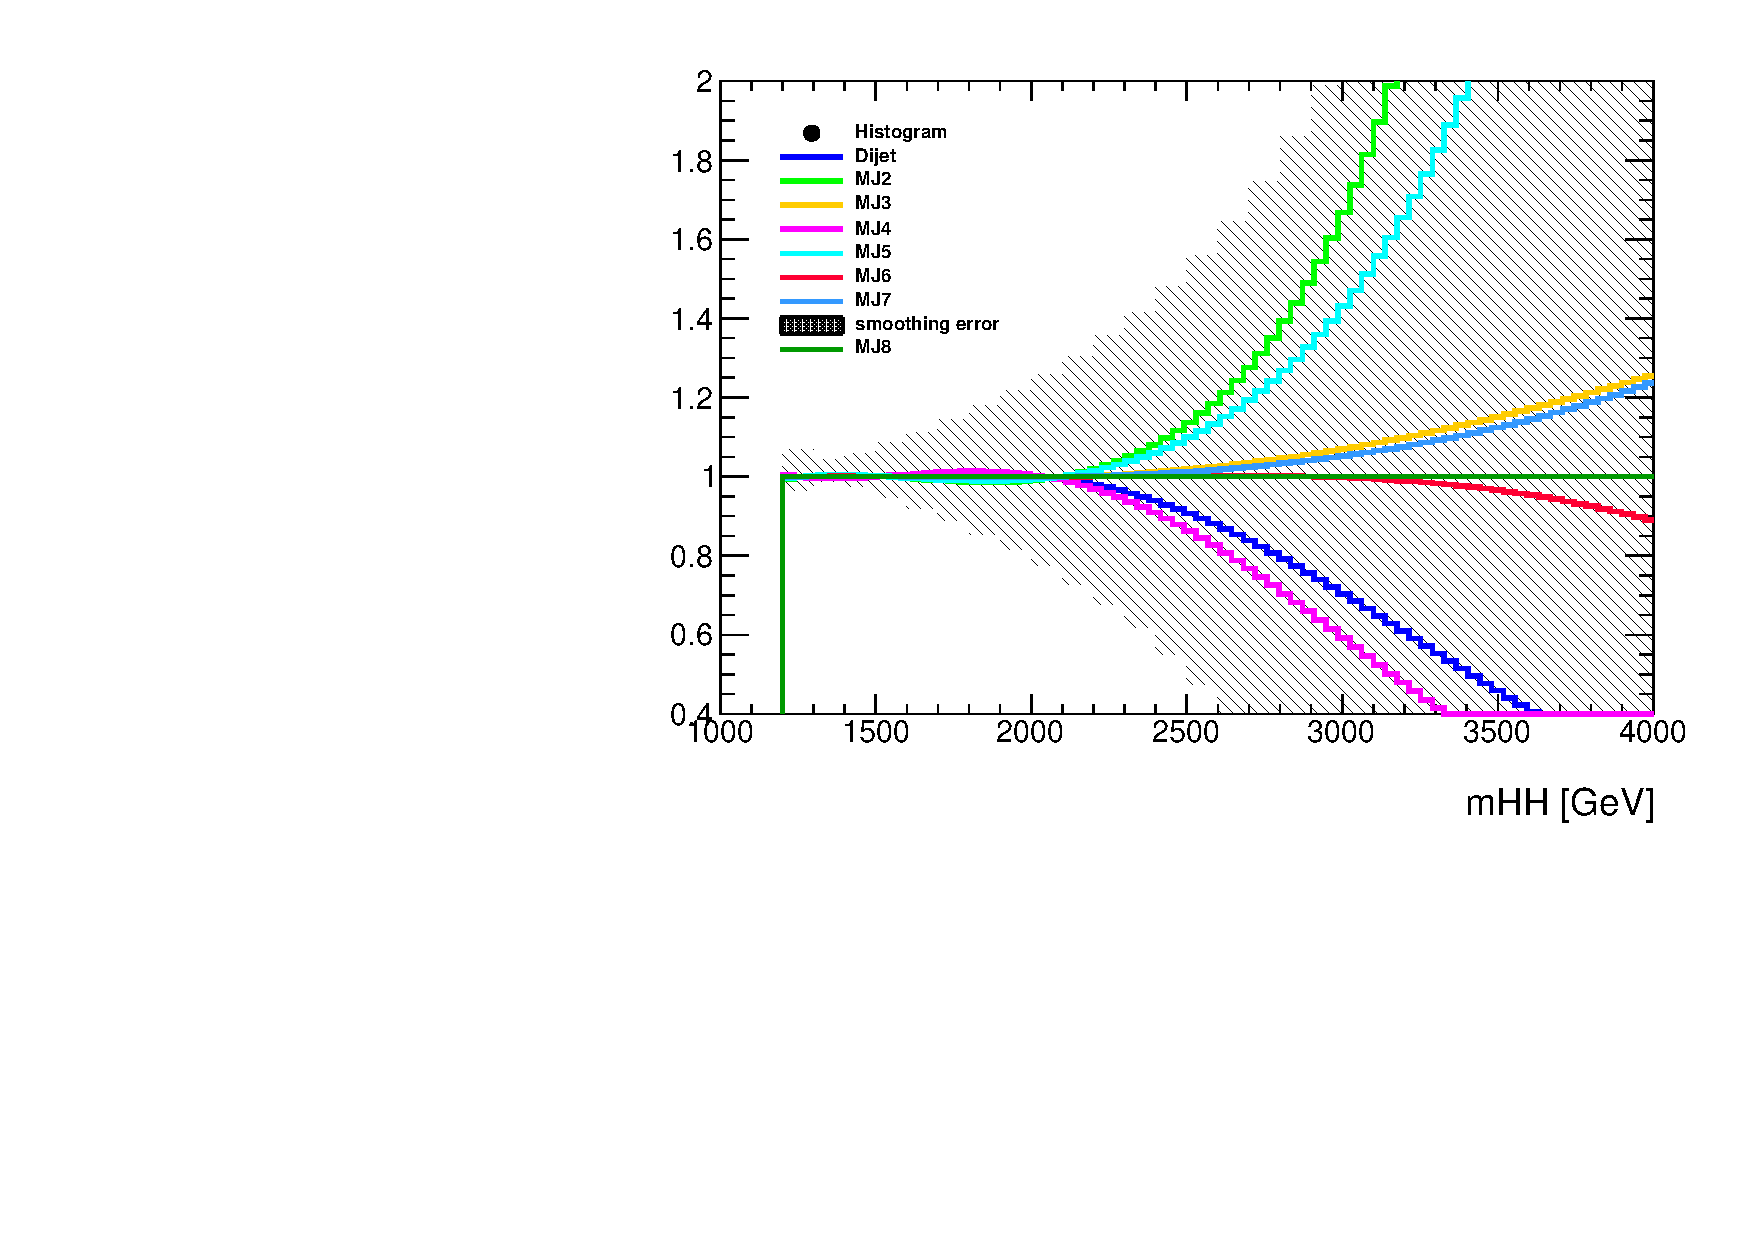
\includegraphics[width=0.31\textwidth,angle=-90]{figures/boosted/Syst_Smooth/smoothFuncCompare_44_comp_ratio.pdf} \\
\caption{ Dijet mass distribution SR prediction fit with several fit functions (left) and the ratio of nominal to fits with different fit functions (right)  for the $2bs$ (top) $3b$ (middle) and $4b$ (bottom) samples. The additional fit functions are from Table~\ref{tab:fit_funcs}.}
\label{fig:qcd_fit_funcs_sys}
\end{center}
\end{figure}

%%%%%%%%%%%%%%%%%%%%%%%%%%%%%%%%%%%%%%%%%%%%%%%%%%%%%%%%%%%%%%%%%%%%%%%
%%%%%%%%%%%%%%%%%%%%%%%%%%%%%%%%%%%%%%%%%%%%%%%%%%%%%%%%%%%%%%%%%%%%%%%

\section{Summary of systematics}
\label{sec:boosted-systematics-numbers}

\paragraph{}
Table~\ref{tab:summary-systematics-4b} shows the percent impact of systematics used in the boosted analysis on the backgrounds yields and on the expected yields for RSG $c=1.0$ signals in the $4b$ signal region.
The correspondent values are shown for the $3b$ signal region in Table ~\ref{tab:summary-systematics-3b}, and are shown for the $2bs$ signal region in Table ~\ref{tab:summary-systematics-2b}.
The systematics that have no impact the yield are not listed. 
These are uncertainties on the shape of the QCD and \ttbar~ backgrounds in the signal region.

\paragraph{}
The ``Background Normalization Fit'' uncertainty comes from summing in quadrature the independent uncertainty components calculated from the correlated statistical errors of \muqcd and \alphatt. 
The ``QCD Non-Closure in CR'' systematic is derived as the maximum of the difference between the predicted and observed $4b/3b/2bs$ QCD yields in the control region, or the fractional change in SR predictions from varying the CR and SB definitions.
Both options gave similar sized uncertainties, but the uncertainty from the CR/SB variations was found to be larger. 
All these uncertainties are summed in quadrature and shown in the ``Bkg Est'' row in the table.

\paragraph{}
The size of the Monte Carlo modeling systematics on the \Grav with $c=1.0$ yield as a function of the signal mass can be found in Figure~\ref{fig:signal_syst_summary}. 
These uncertainties have a similar impact on the other signals. 
The largest uncertainty in the $4b$ and $2b$ signal region is from $b$-tagging, followed by the JMR uncertainty.
In the $3b$ signal region, although $b$-tagging systematics is still one of the largest uncertainty, it has been much reduced compared to $4b$ region, as discussed in Section~\ref{sec:b-tagging-unc}. 

\begin{figure}[htbp!]
\begin{center}
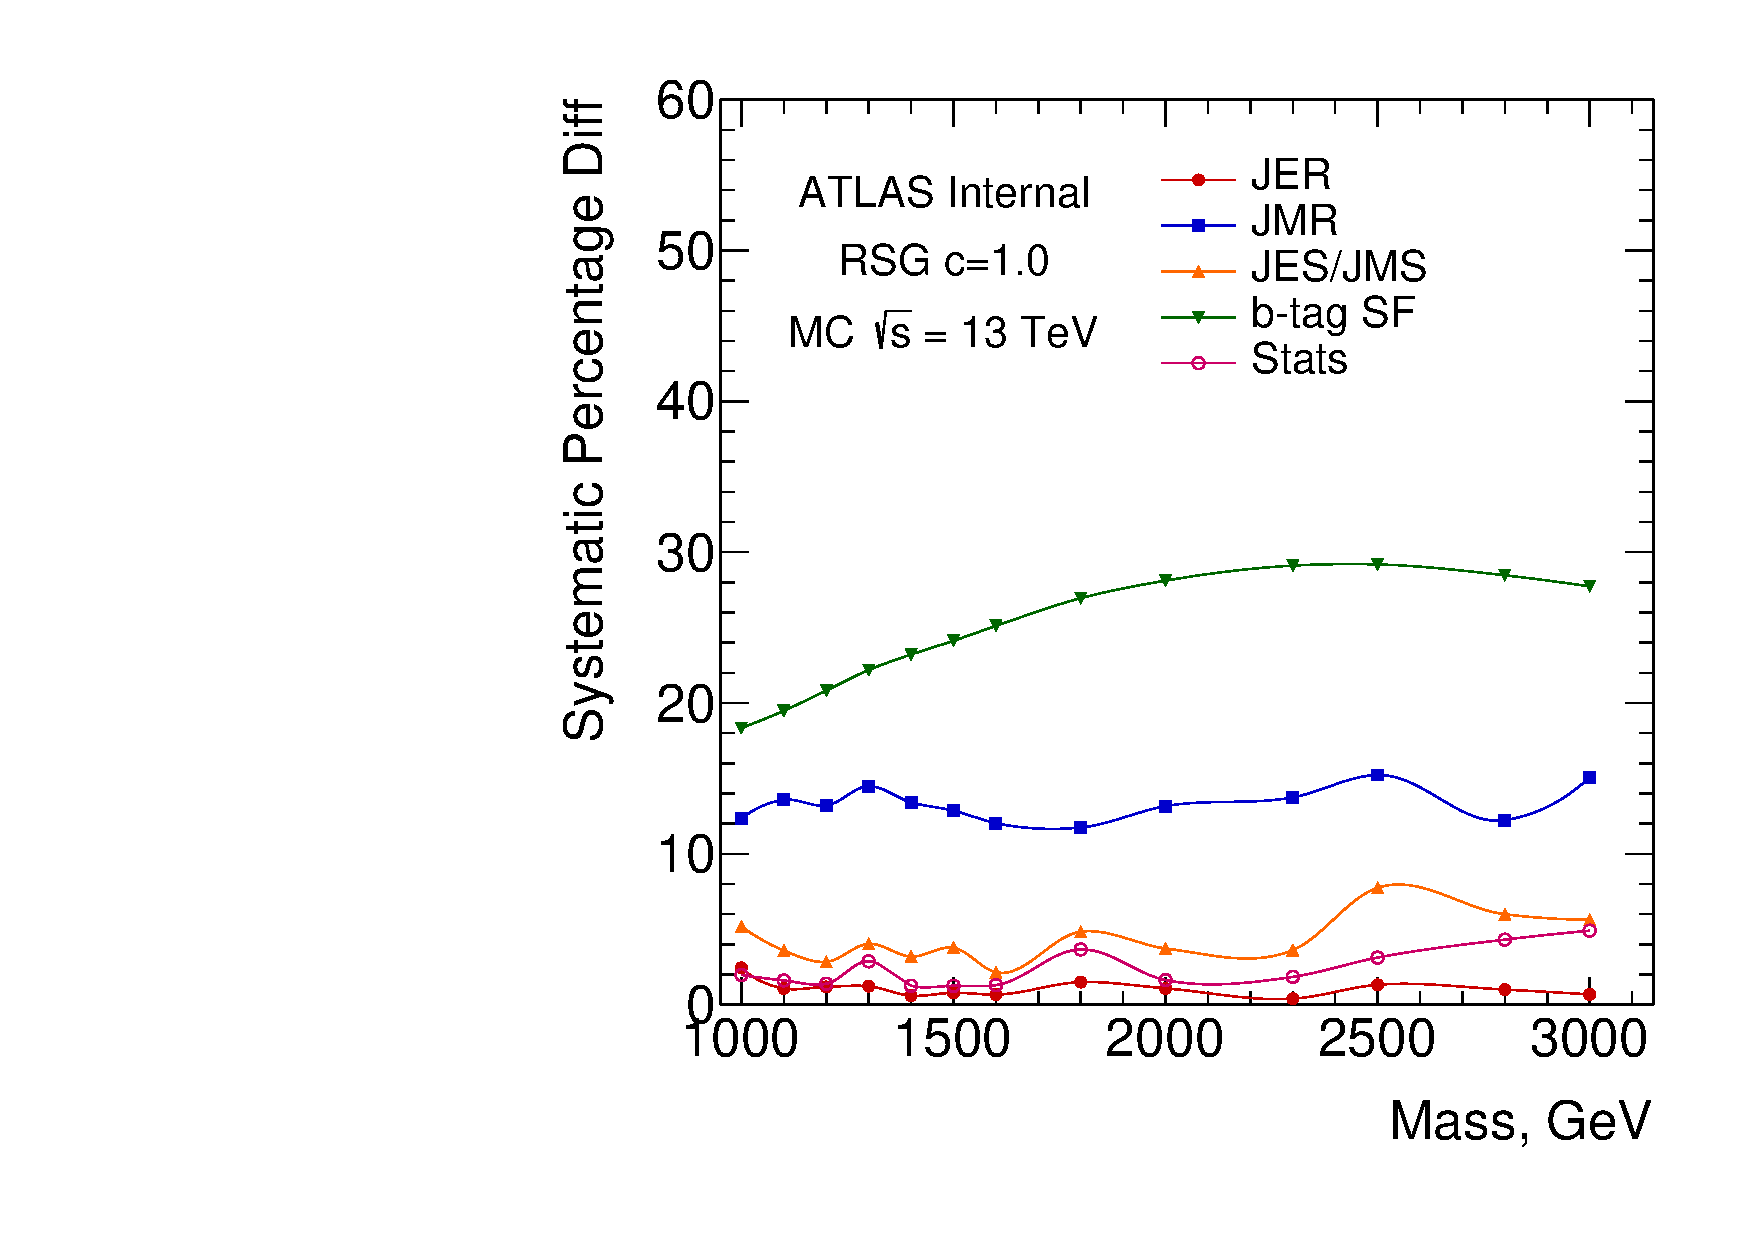
\includegraphics[width=0.31\textwidth,angle=-90]{figures/boosted/Syst_MC/FourTag_RSG_syst.pdf}
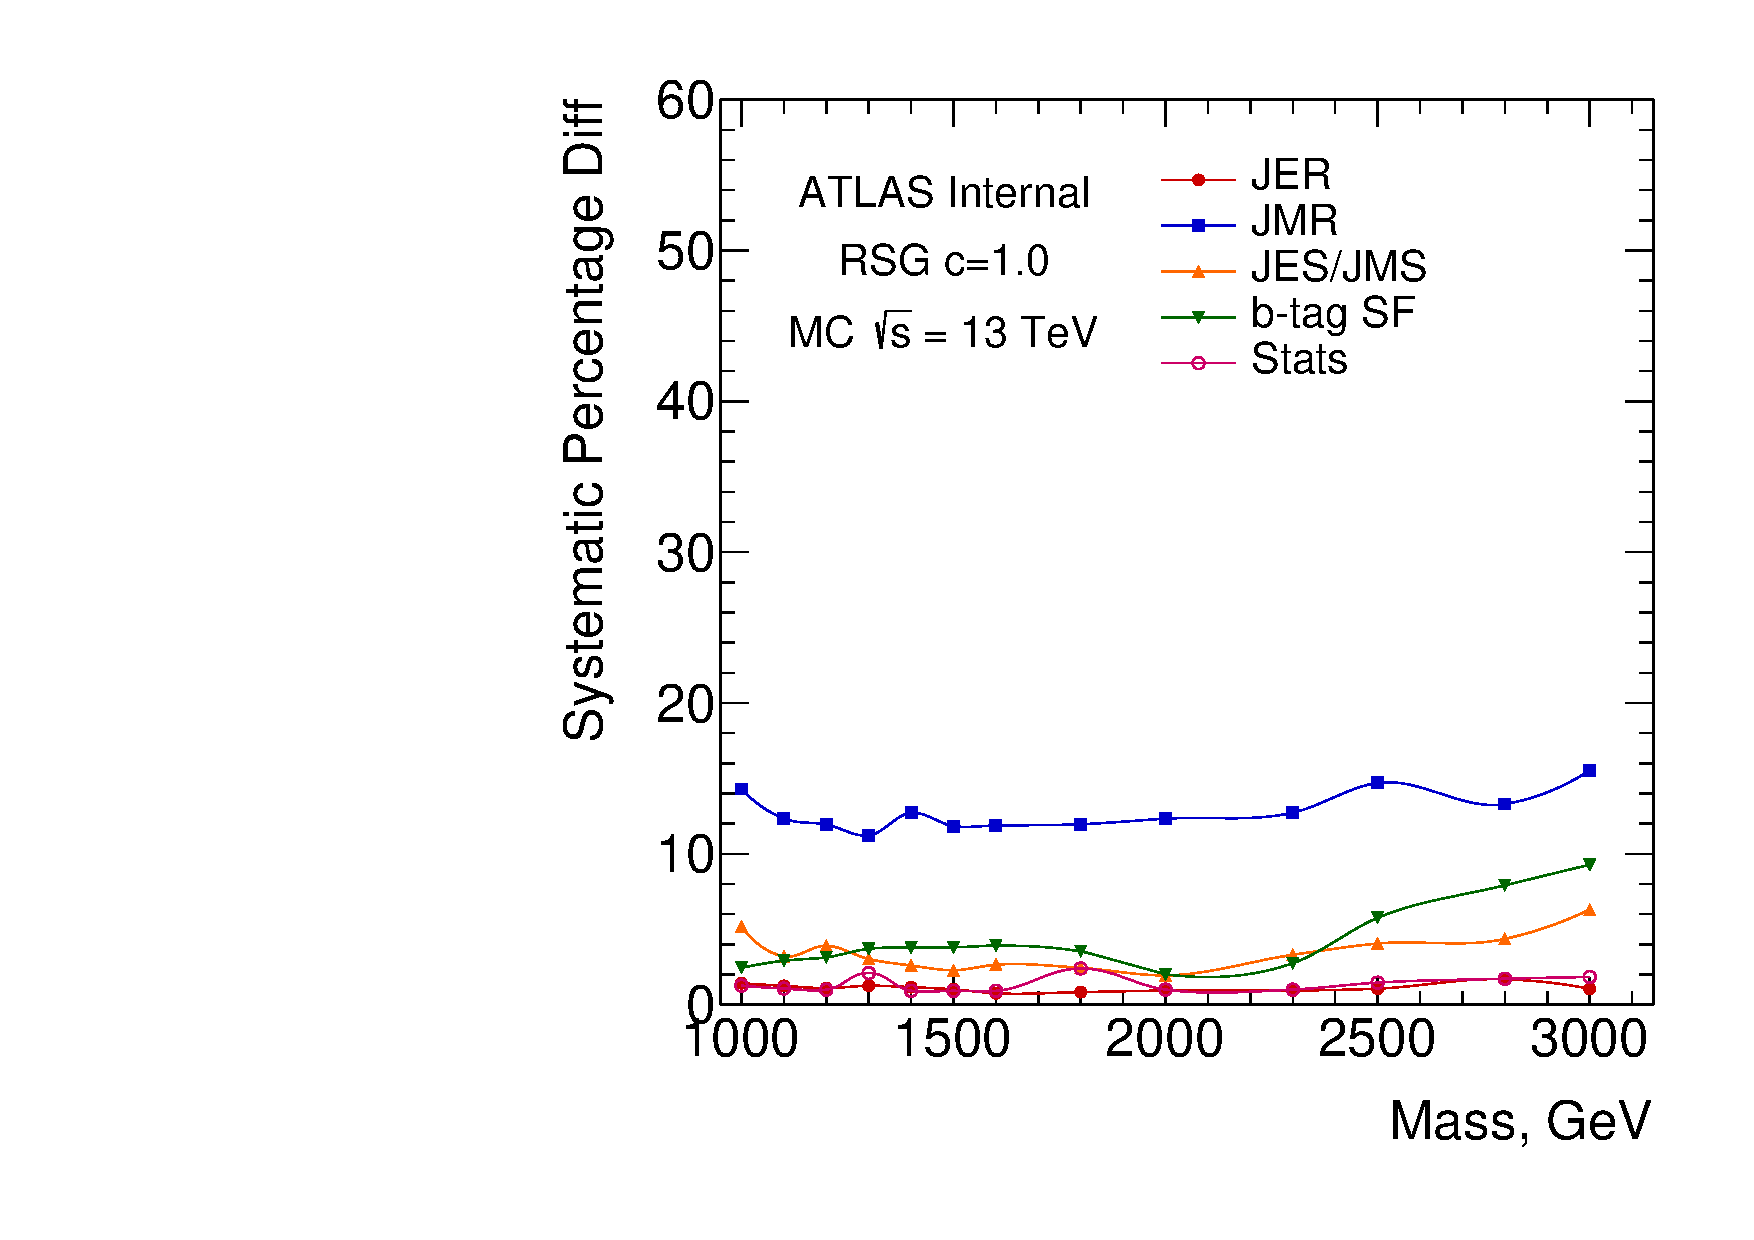
\includegraphics[width=0.31\textwidth,angle=-90]{figures/boosted/Syst_MC/ThreeTag_RSG_syst.pdf}
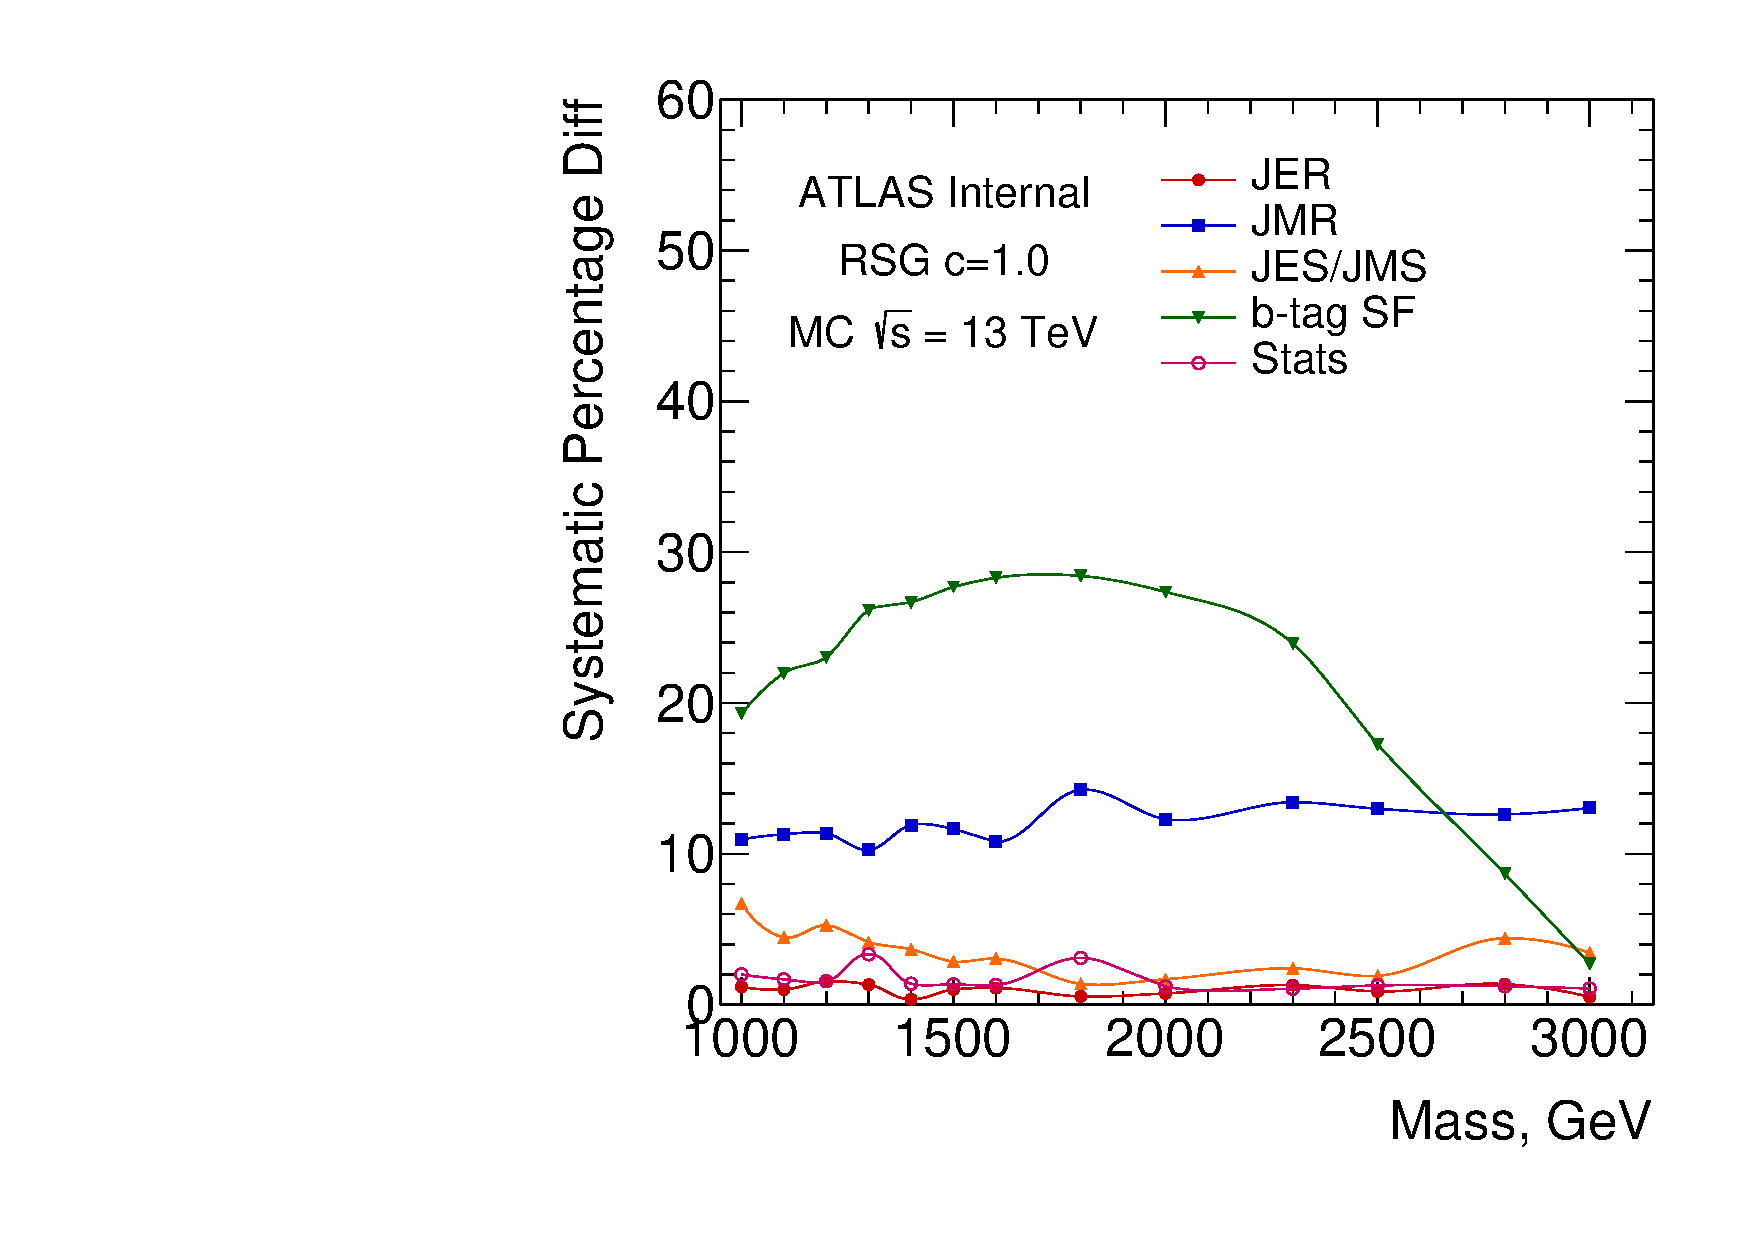
\includegraphics[width=0.31\textwidth,angle=-90]{figures/boosted/Syst_MC/TwoTag_split_RSG_syst.pdf}
\caption{Impact of each systematic on the signal prediction as a function of the signal mass, in the $4b$ (left) and $3b$ (middle) and $2bs$ signal regions.}
\label{fig:signal_syst_summary}
\end{center}
\end{figure}

\begin{table}[htbp!]
\scriptsize
\begin{center}
\caption{Percent impact of the dominant systematics on the background acceptance
         and on the signal acceptance of \Grav with $c=1.0$ in the $4b$ signal region.}
\begin{footnotesize} 
\begin{tabular}{c|c|c|c|c|c|c} 
FourTag & totalbkg & qcd & ttbar & RSG1 1000 & RSG1 2000 & RSG1 3000 \\ 
\hline\hline 
JER & 0.45 & 0.27 & 3.98 & 2.44 & 1.07 & 0.67\\ 
JMR & 7.9 & 10.35 & 39.95 & 12.33 & 13.16 & 15.08\\ 
Top &  -  &  -  &  -  &  -  &  -  &  - \\ 
JES/JMS & 1.32 & 1.49 & 24.36 & 5.18 & 3.72 & 5.62\\ 
Bkg Est & 15.67 & 18.19 & 67.82 &  -  &  -  &  - \\ 
b-tag SF & 1.11 & 0.79 & 18.85 & 18.34 & 28.11 & 27.73\\ 
\hline 
Total Sys & 17.64 & 21.0 & 84.62 & 22.83 & 31.28 & 32.07\\ 
\hline 
Stat & 3.13 & 3.29 & 2.47 & 1.97 & 1.63 & 4.9\\ 
\hline 
Estimated Events & 34.59 & 32.91 & 1.68 & 10.07 & 0.25 & 0.0016\\ 
\hline\hline 
\end{tabular} 
\end{footnotesize} 
\newline 

\label{tab:summary-systematics-4b}
\end{center}
\end{table}

\begin{table}[htbp!]
\scriptsize
\begin{center}
\caption{Percent impact of the dominant systematics on the background acceptance
         and on the signal acceptance of \Grav with $c=1.0$ in the $3b$ signal region.}
\begin{footnotesize} 
\begin{tabular}{c|c|c|c|c|c|c} 
ThreeTag & totalbkg & qcd & ttbar & RSG1 1000 & RSG1 2000 & RSG1 3000 \\ 
\hline\hline 
JER & 1.38 & 3.52 & 17.5 & 1.41 & 0.93 & 1.08\\ 
JMR & 1.35 & 4.26 & 24.38 & 14.3 & 12.33 & 15.53\\ 
Top &  -  &  -  &  -  &  -  &  -  &  - \\ 
JES/JMS & 2.03 & 1.26 & 26.22 & 5.19 & 1.94 & 6.35\\ 
Bkg Est & 4.84 & 5.62 & 9.45 &  -  &  -  &  - \\ 
b-tag SF & 0.47 & 0.53 & 8.45 & 2.45 & 2.01 & 9.27\\ 
\hline 
Total Sys & 5.61 & 8.0 & 41.82 & 15.47 & 12.68 & 19.2\\ 
\hline 
Stat & 1.32 & 1.44 & 2.47 & 1.26 & 1.0 & 1.83\\ 
\hline 
Estimated Events & 780.89 & 701.52 & 79.38 & 26.0 & 0.76 & 0.013\\ 
\hline\hline 
\end{tabular} 
\end{footnotesize} 
\newline 

\label{tab:summary-systematics-3b}
\end{center}
\end{table}

\begin{table}[htbp!]
\scriptsize
\begin{center}
\caption{Percent impact of the dominant systematics on the background acceptance
         and on the signal acceptance of \Grav with $c=1.0$ in the $2bs$ signal region.}
\begin{footnotesize} 
\begin{tabular}{c|c|c|c|c|c|c} 
TwoTag split & totalbkg & qcd & ttbar & RSG1 1000 & RSG1 2000 & RSG1 3000 \\ 
\hline\hline 
JER & 0.25 & 0.48 & 3.14 & 1.18 & 0.74 & 0.5\\ 
JMR & 0.52 & 1.73 & 9.43 & 10.96 & 12.3 & 13.05\\ 
Top & 4.82 & 6.98 & 26.63 &  -  &  -  &  - \\ 
JES/JMS & 0.43 & 1.67 & 7.17 & 6.72 & 1.69 & 3.44\\ 
Bkg Est & 2.76 & 3.38 & 2.35 &  -  &  -  &  - \\ 
b-tag SF & 0.83 & 1.43 & 1.82 & 19.28 & 27.36 & 2.7\\ 
\hline 
Total Sys & 5.66 & 8.26 & 29.46 & 23.2 & 30.05 & 13.77\\ 
\hline 
Stat & 0.6 & 0.42 & 2.48 & 2.0 & 1.2 & 1.07\\ 
\hline 
Estimated Events & 4252.44 & 3393.74 & 858.7 & 10.87 & 0.6 & 0.039\\ 
\hline\hline 
\end{tabular} 
\end{footnotesize} 
\newline 

\label{tab:summary-systematics-2b}
\end{center}
\end{table}


% \paragraph{}
% The final background prediction of scaled \mtwoJ along with total uncertainties can be found in Figure~\ref{fig:FinalBkg_sys-4b-pole}, ~\ref{fig:FinalBkg_sys-3b-pole}, and ~\ref{fig:FinalBkg_sys-2b-pole}.

% \begin{figure}
% \begin{center}
% 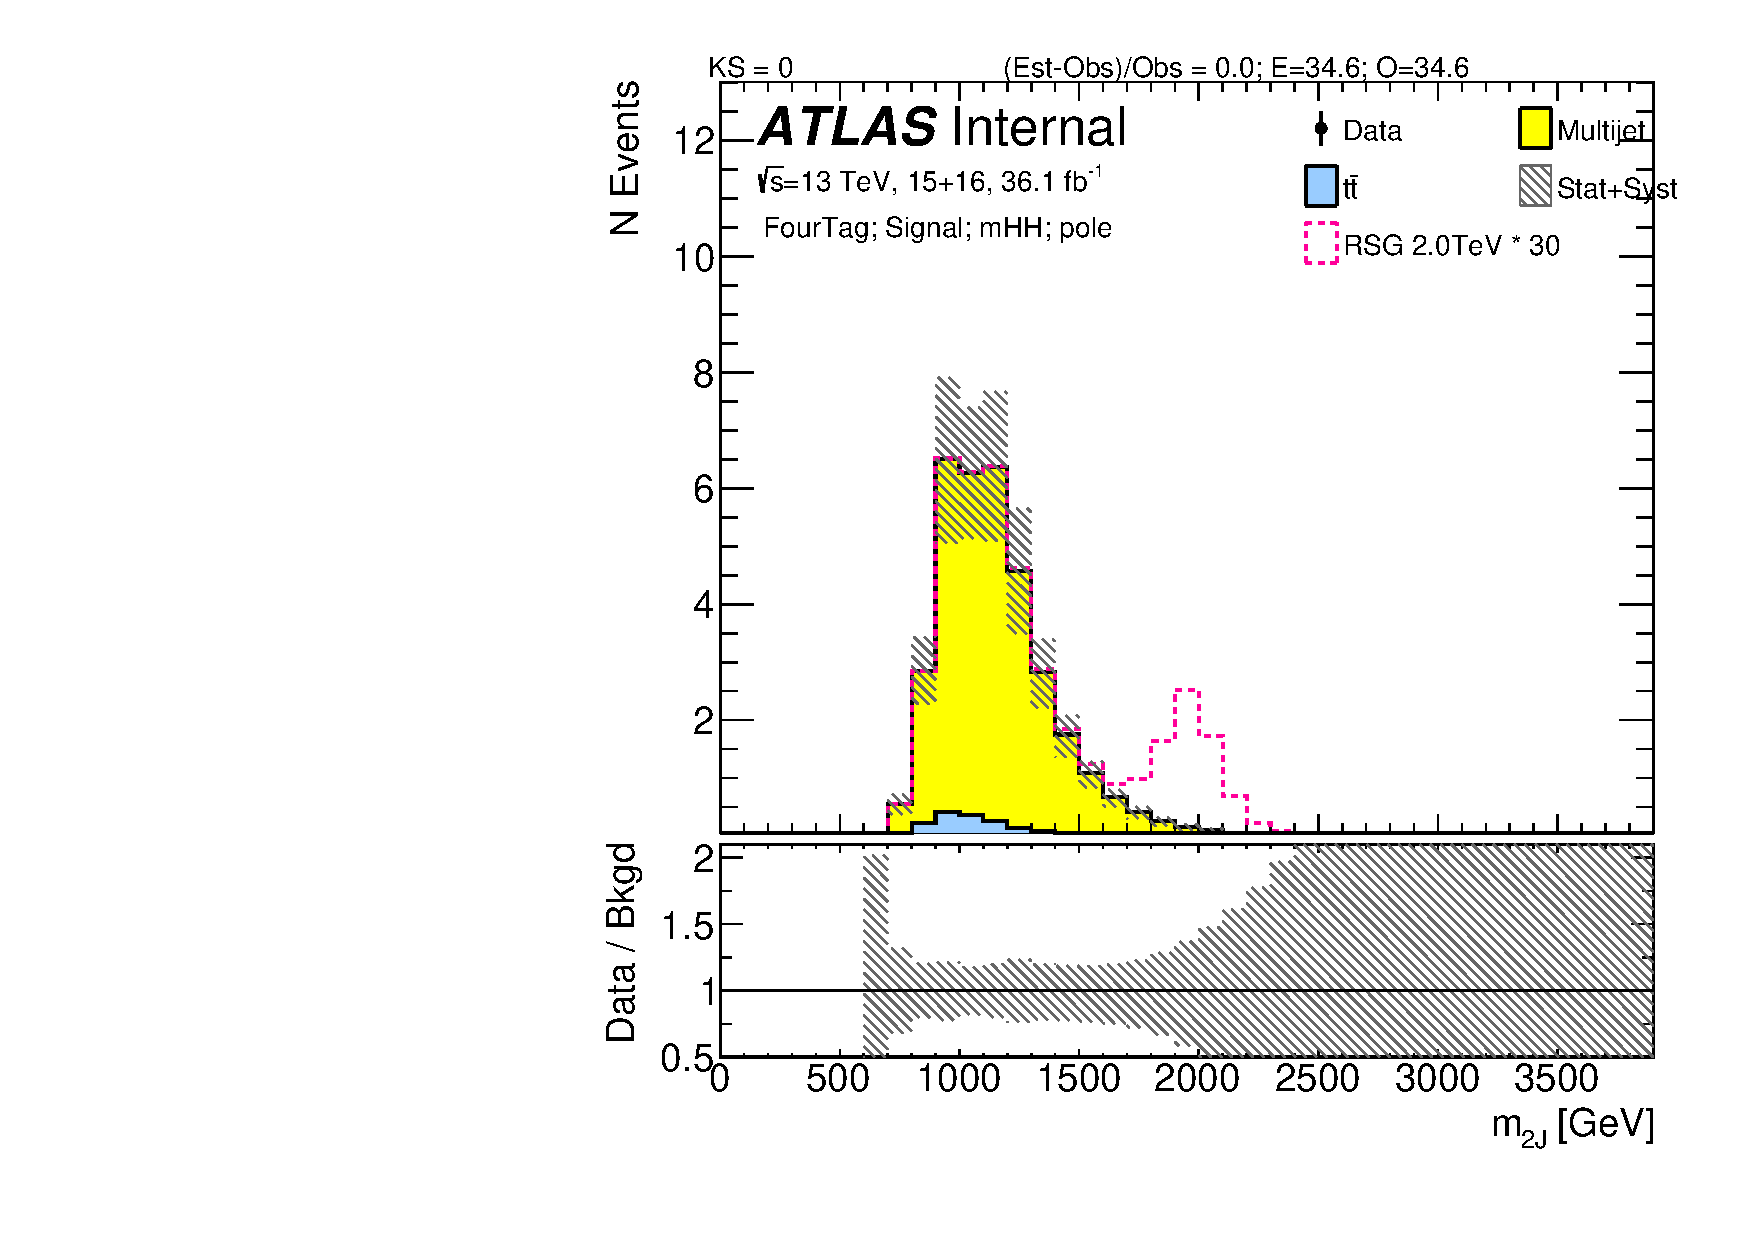
\includegraphics[width=0.48\textwidth,angle=-90]{figures/boosted/Signal_Syst/Moriond_bkg_9_FourTag_Signal_mHH_pole_blind.pdf}
% 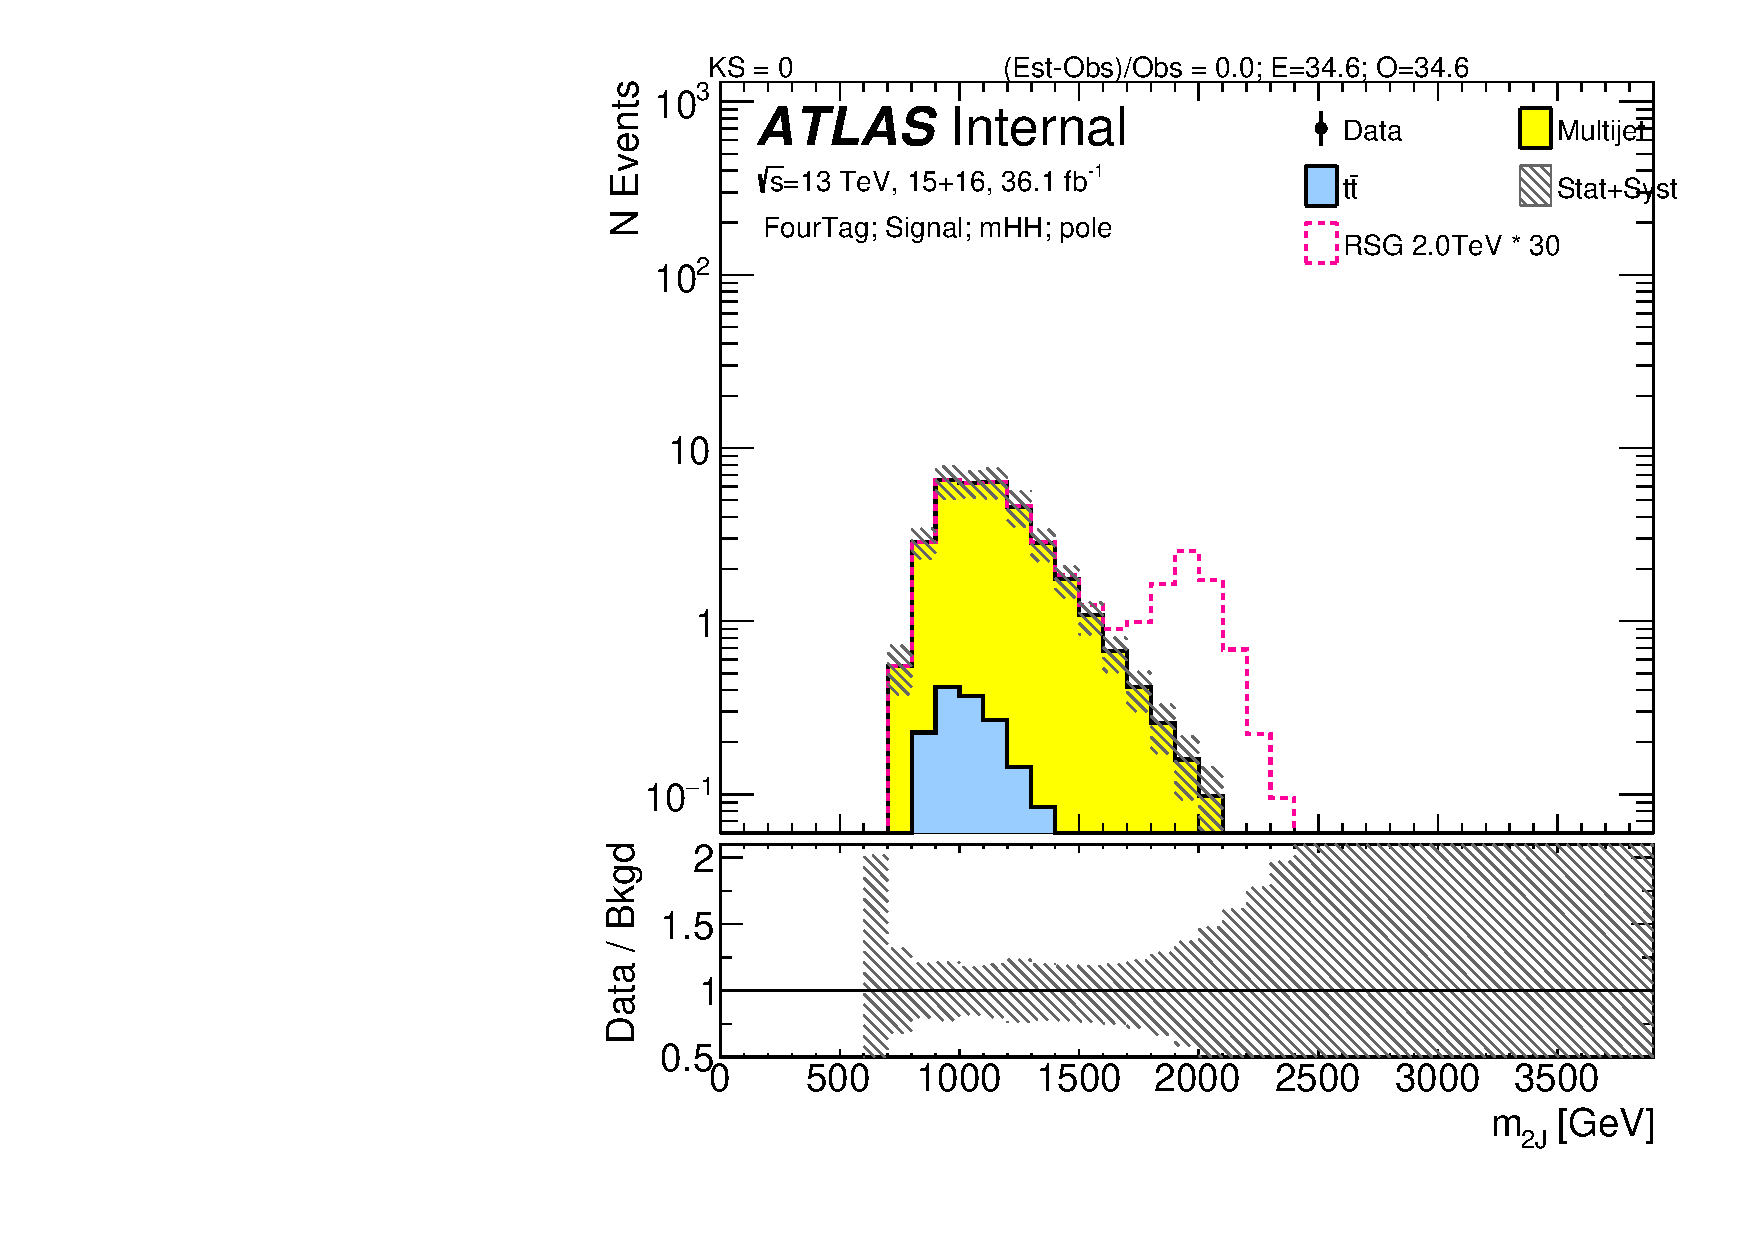
\includegraphics[width=0.48\textwidth,angle=-90]{figures/boosted/Signal_Syst/Moriond_bkg_9_FourTag_Signal_mHH_pole_1_blind.pdf}
% \caption{The total background estimation in $4b$ signal region, scaled mJJ, with linear scale on the left and with log scale on the right, along with total uncertainties (stats.$+$systematic) variation up and down.}
% \label{fig:FinalBkg_sys-4b-pole}
% \end{center}
% \end{figure}


% \begin{figure}
% \begin{center}
% 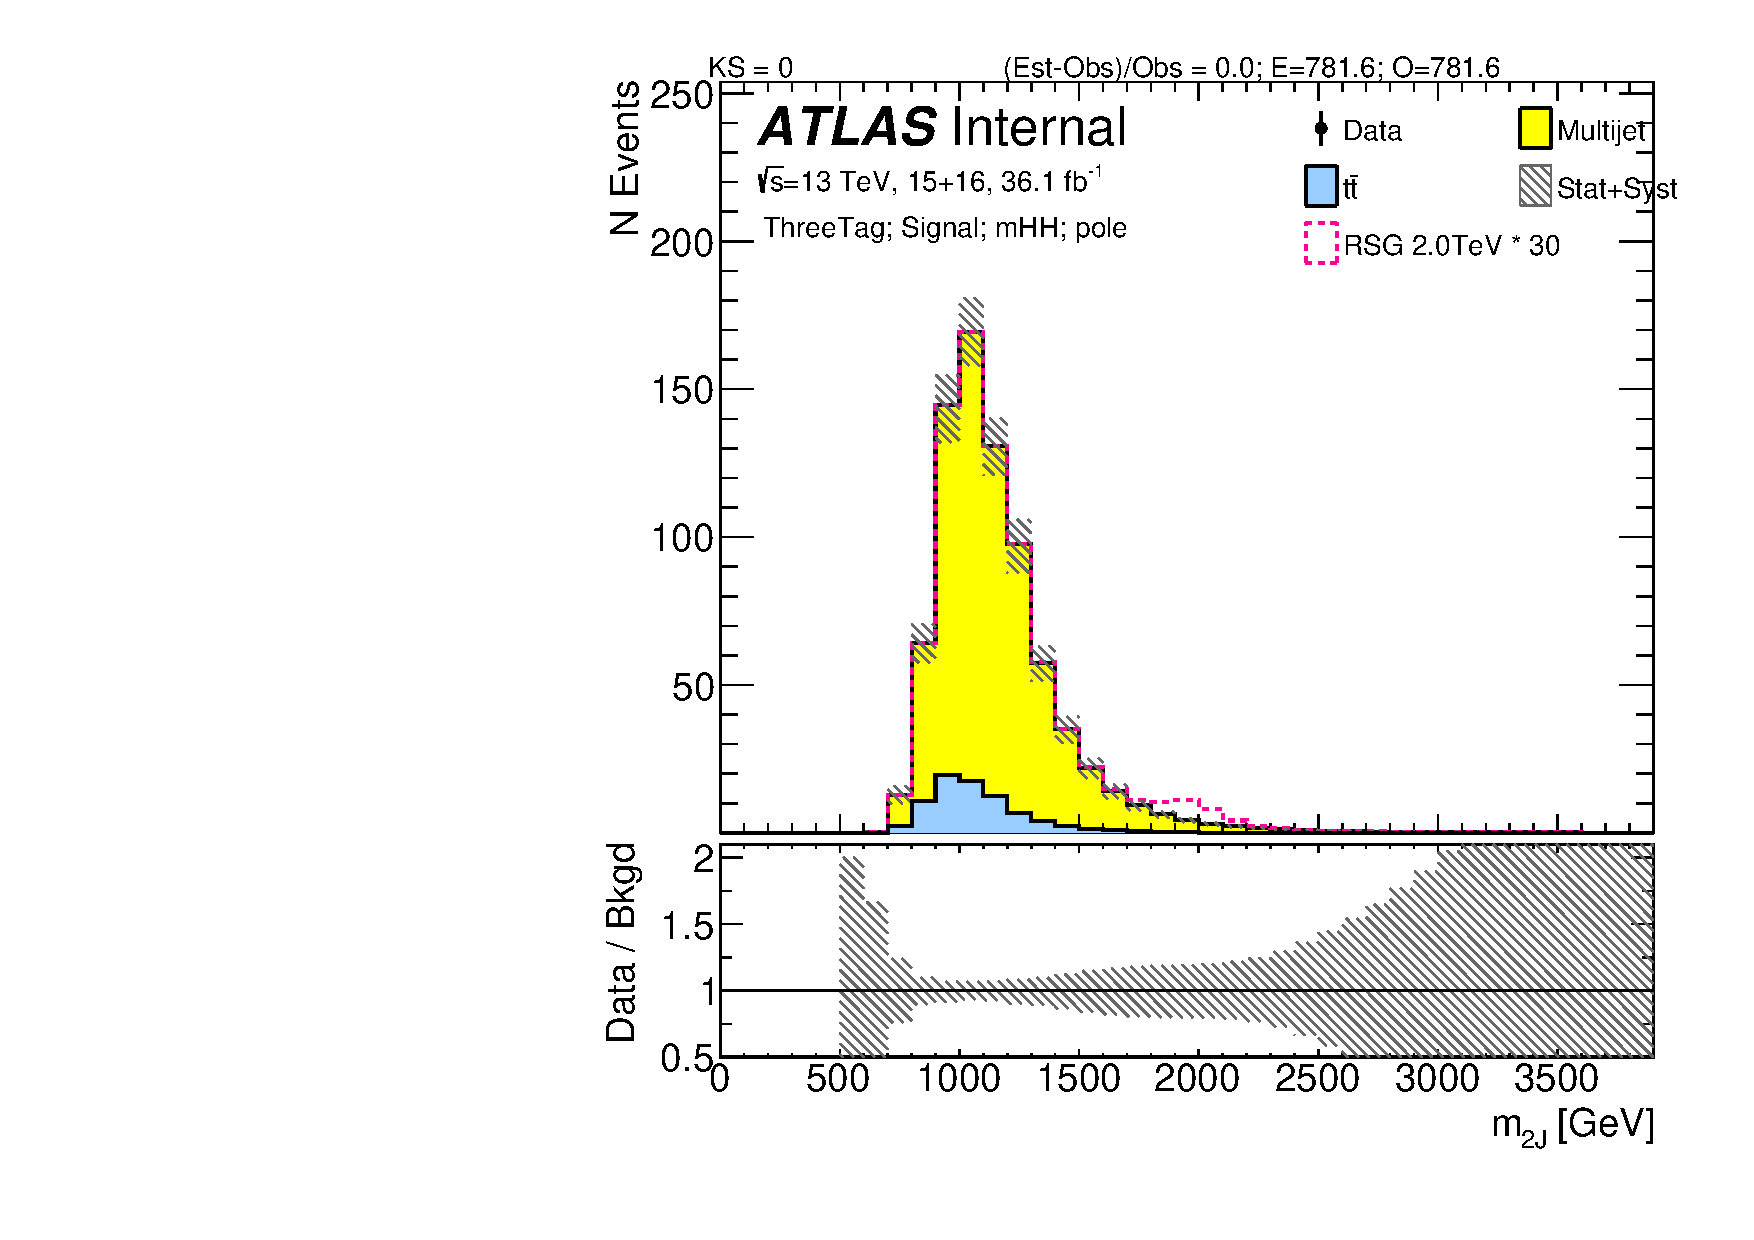
\includegraphics[width=0.48\textwidth,angle=-90]{figures/boosted/Signal_Syst/Moriond_bkg_9_ThreeTag_Signal_mHH_pole_blind.pdf}
% 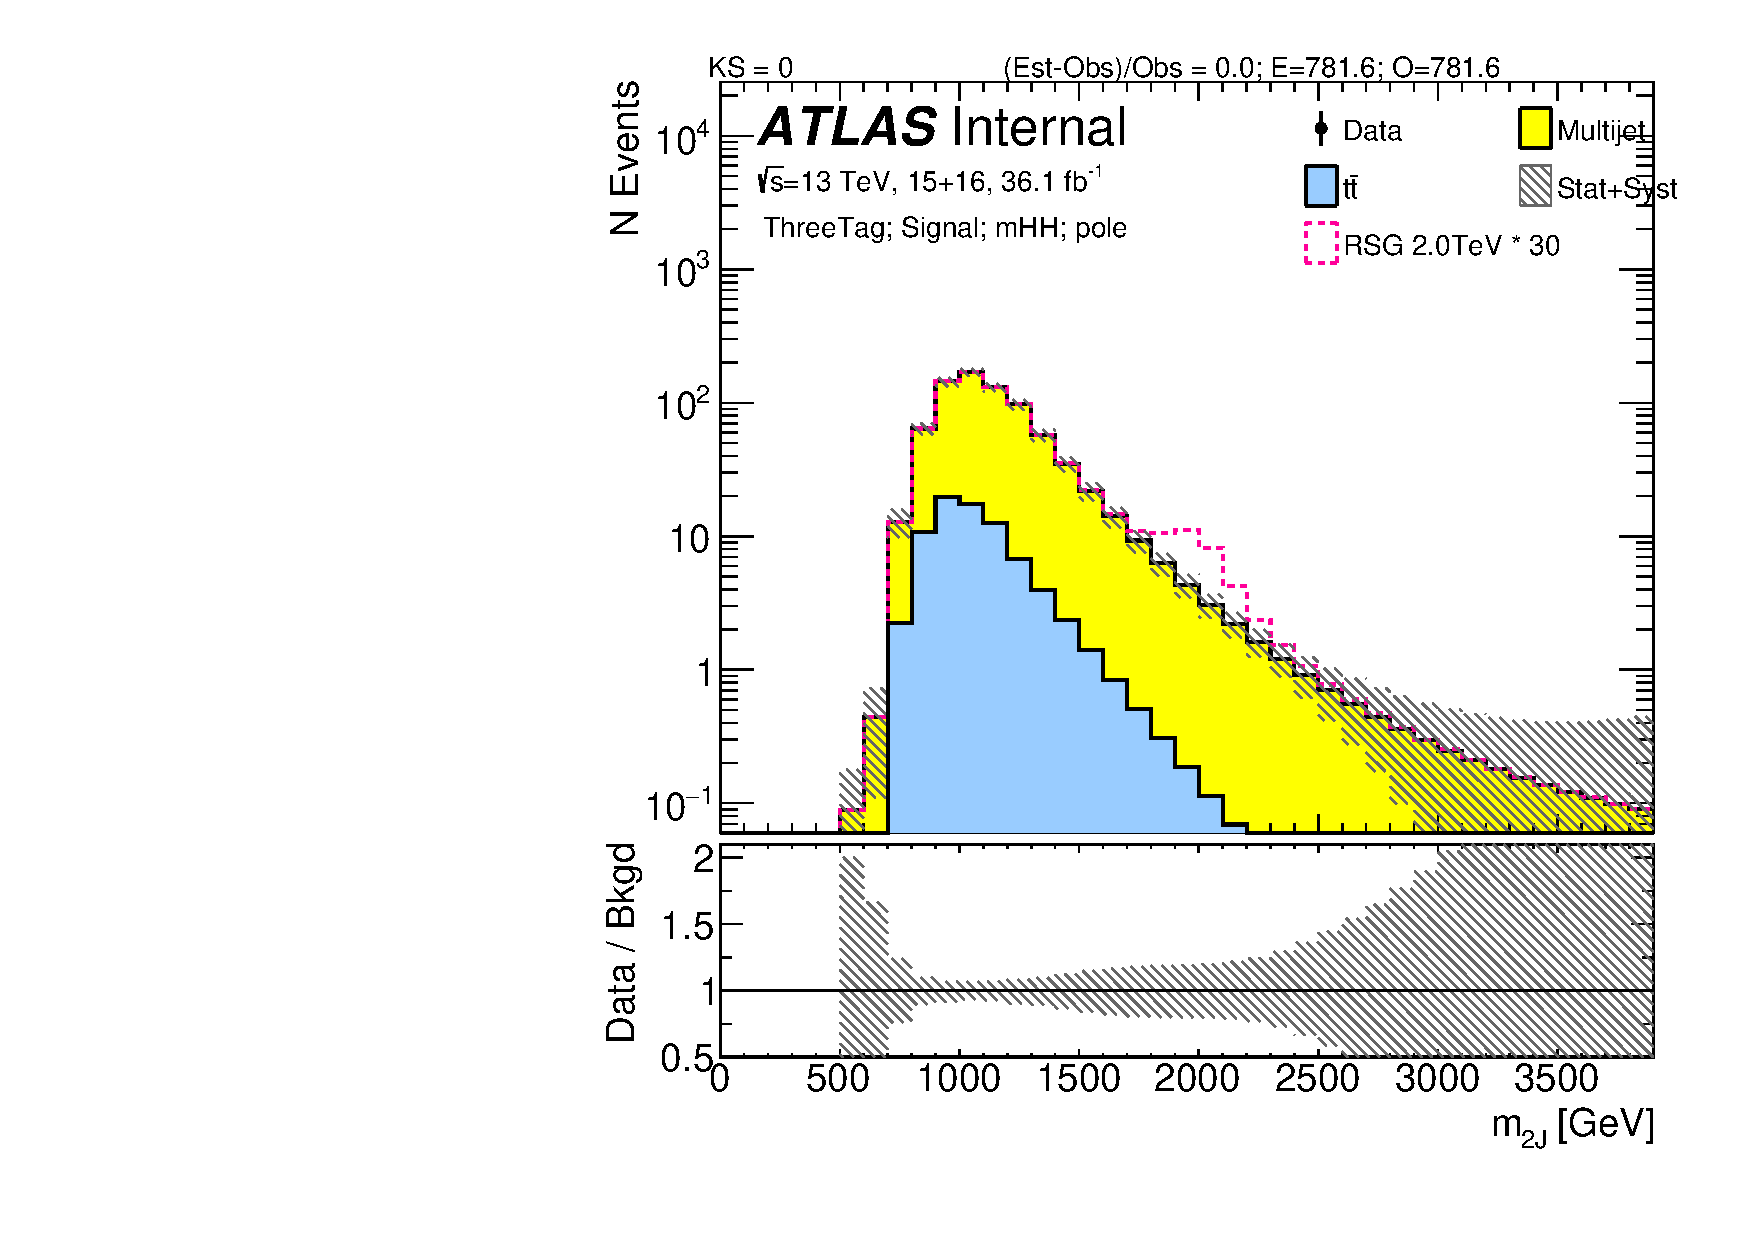
\includegraphics[width=0.48\textwidth,angle=-90]{figures/boosted/Signal_Syst/Moriond_bkg_9_ThreeTag_Signal_mHH_pole_1_blind.pdf}
% \caption{The total background estimation in $3b$ signal region, scaled mJJ, with linear scale on the left and with log scale on the right, along with total uncertainties (stats.$+$systematic) variation up and down.}
% \label{fig:FinalBkg_sys-3b-pole}
% \end{center}
% \end{figure}


% \begin{figure}
% \begin{center}
% 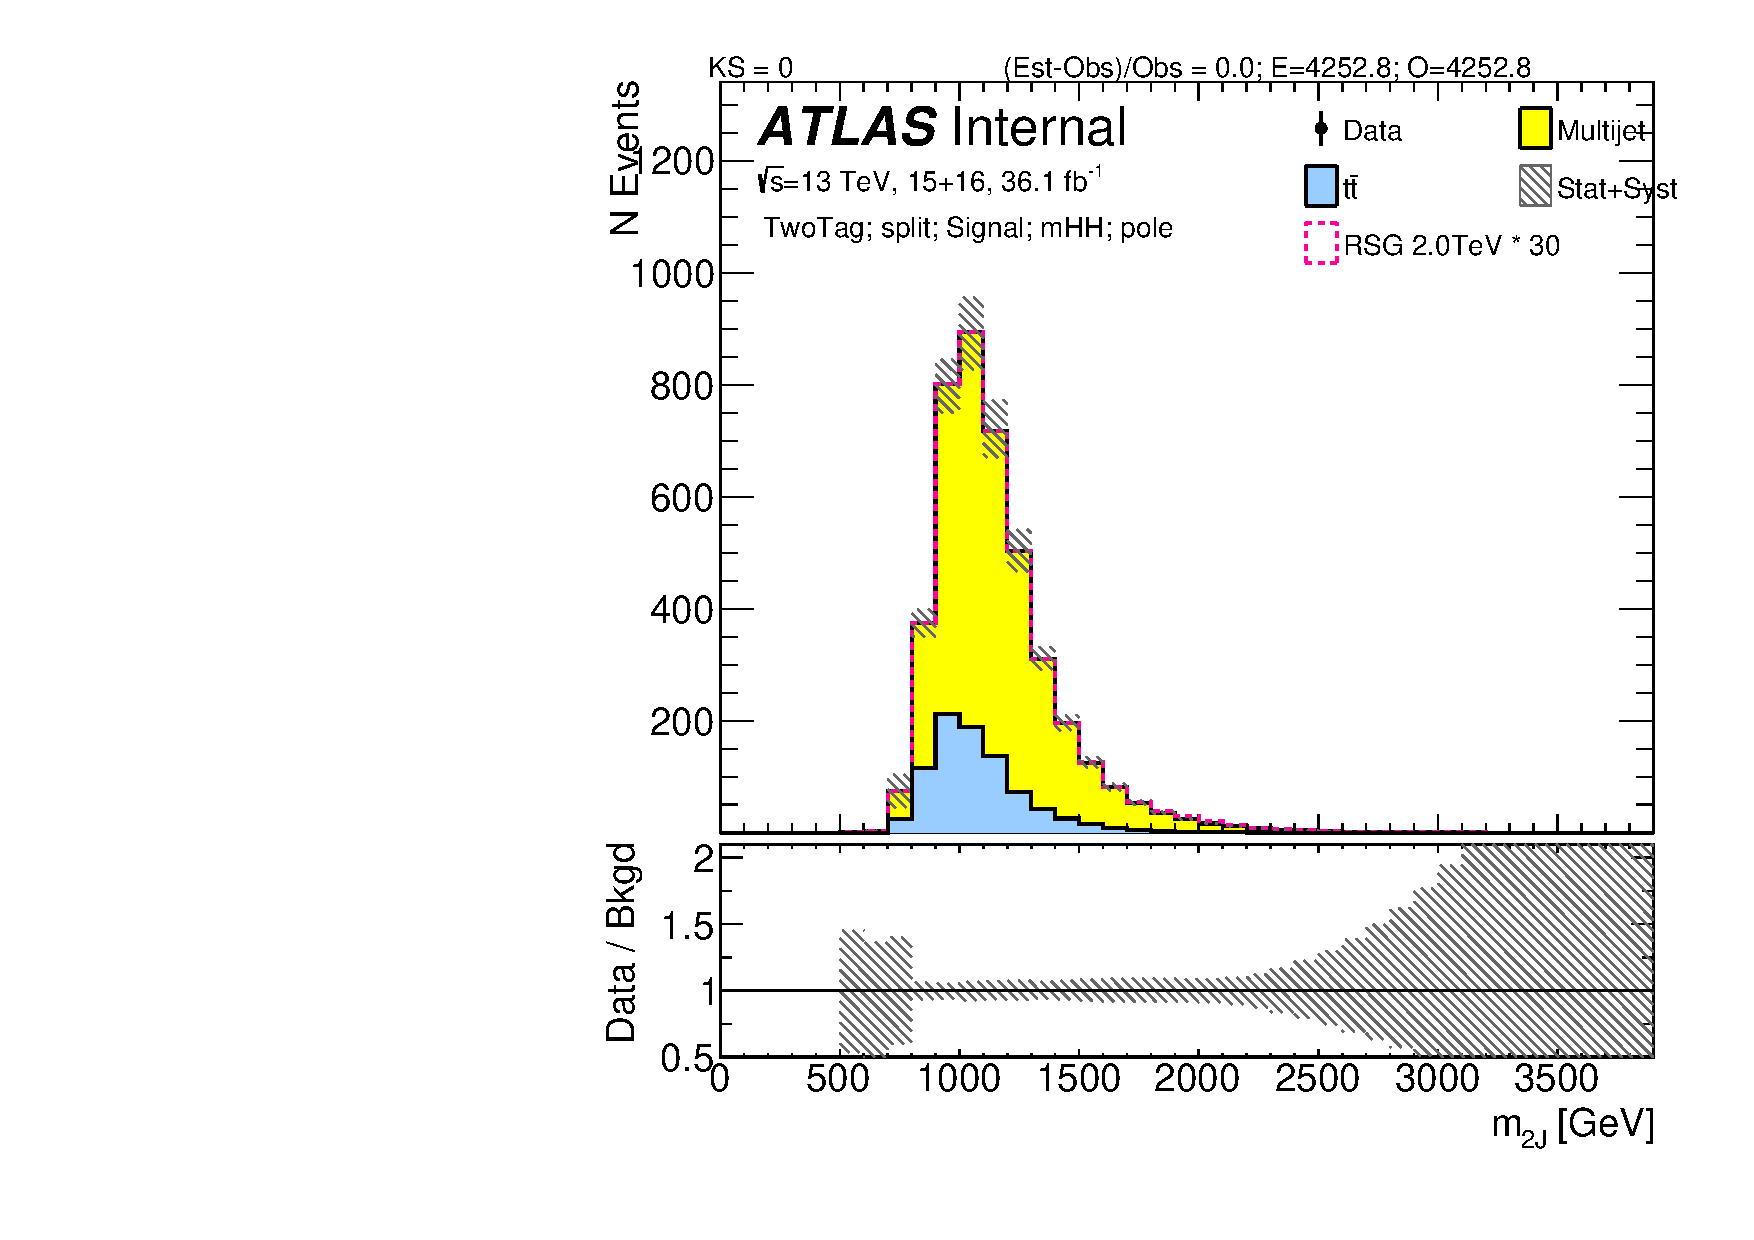
\includegraphics[width=0.48\textwidth,angle=-90]{figures/boosted/Signal_Syst/Moriond_bkg_9_TwoTag_split_Signal_mHH_pole_blind.pdf}
% 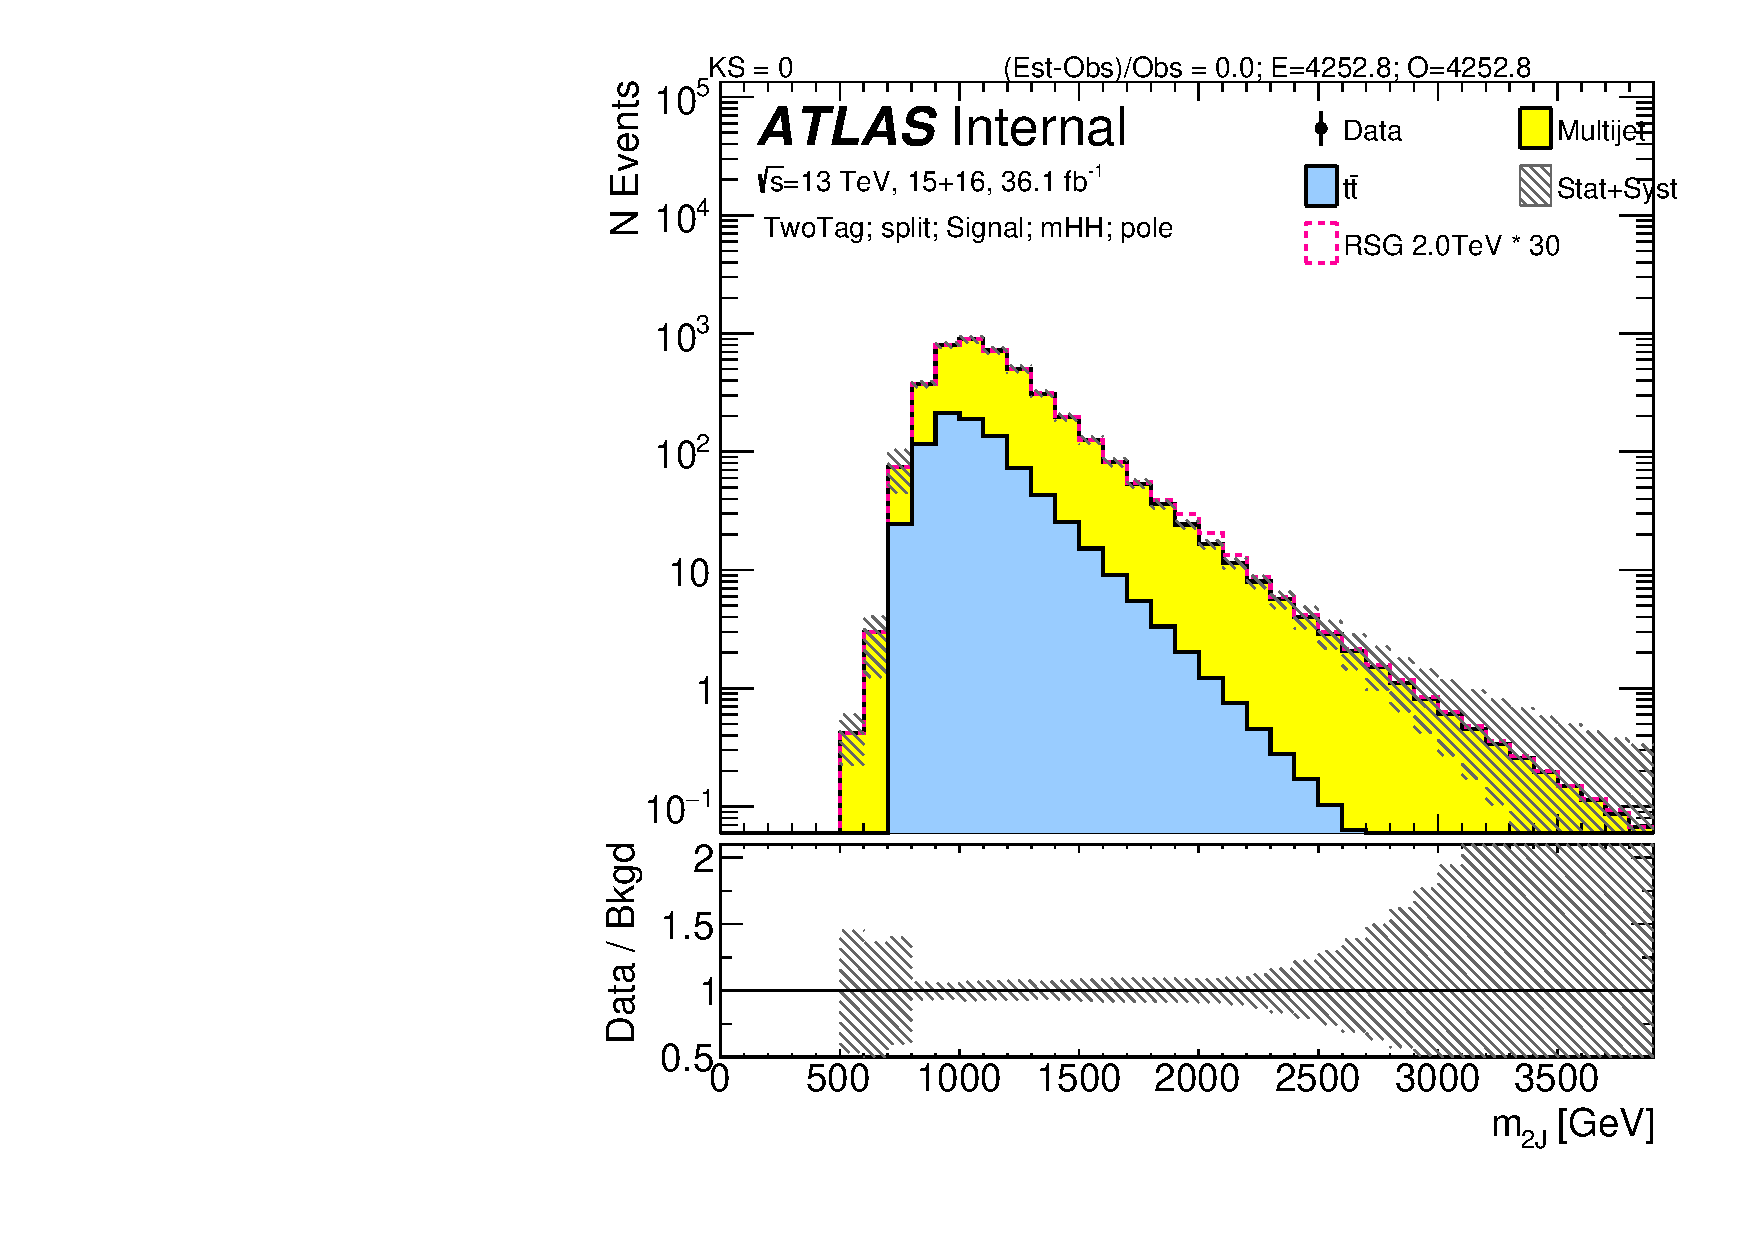
\includegraphics[width=0.48\textwidth,angle=-90]{figures/boosted/Signal_Syst/Moriond_bkg_9_TwoTag_split_Signal_mHH_pole_1_blind.pdf}
% \caption{The total background estimation in $2bs$ signal region, scaled mJJ, with linear scale on the left and with log scale on the right, along with total uncertainties (stats.$+$systematic) variation up and down.}
% \label{fig:FinalBkg_sys-2b-pole}
% \end{center}
% \end{figure}


%%%%%%%%%%%%%%%%%%%%%%%%%%%%%%%%%%%%%%%%%%%%%%%%%%%%%%%%%%%%%%%%%%%%%%%
%%%%%%%%%%%%%%%%%%%%%%%%%%%%%%%%%%%%%%%%%%%%%%%%%%%%%%%%%%%%%%%%%%%%%%%